%Gilmore Space LaTeX template
%Rory Kelly ~ 21 Nov 2024
%Needed for ?. Must come before document class
\RequirePackage{pdfmanagement-testphase}
\DeclareDocumentMetadata{}
\documentclass[12pt]{article}

% Page setup
\usepackage[a4paper]{geometry}

% PDF management (to include PDF pages)
\usepackage{pdfpages}

% Table management (for advanced table formatting)
\usepackage{tabu}

% Font handling
\usepackage{mathspec} 
%\usepackage[no-math]{fontspec} 
\usepackage{fontspec} % for font selection and OpenType/TrueType support

\usepackage[english]{babel} 

% Mathematics support
\usepackage{amsmath, amssymb, amsthm, thmtools}

%\usepackage[no-math]{fontspec} 
%\setmainfont{Gentium Plus} 
%\usepackage[italic]{mathastext}

% Input encoding
\usepackage[utf8]{inputenc}

% File-related commands (for working with file paths)
\usepackage[abspath]{currfile} 

% Section and subsection formatting
\usepackage{titlesec}

% Drawing and custom graphics
\usepackage{tikz} 
%\usetikzlibrary{calc} % Needed for coordinate math

% Watermark management
\usepackage{eso-pic} 

% Header and footer formatting
\usepackage{fancyhdr} 

% Get total number of pages
\usepackage{lastpage}

% Optional package for total page count (not used here)
% \usepackage{zref-totpages} % gets the total page numbers

% Graphics support
\usepackage{graphicx}
\usepackage{float}
\usepackage{transparent} % for transparent watermark

% Hyperlink support
\usepackage[colorlinks, allcolors=blue]{hyperref}

% Table formatting
\usepackage{longtable}
\usepackage{booktabs}
\usepackage{adjustbox}
\usepackage{multirow}
\usepackage{multicol}
\usepackage{array}
\usepackage{tabularx}

% Color support
\usepackage[table, svgnames, dvipsnames]{xcolor}
\definecolor{lightbeige}{RGB}{255, 239, 204}
\definecolor{green}{RGB}{0, 128, 0}
\definecolor{codegreen}{rgb}{0, 0.6, 0}
\definecolor{codegray}{rgb}{0.5, 0.5, 0.5}
\definecolor{codepurple}{rgb}{0.58, 0, 0.82}
\definecolor{backcolour}{rgb}{0.95, 0.95, 0.92}

% Code formatting
\usepackage{verbatim}
\usepackage{listings}
\lstset{
    backgroundcolor=\color{backcolour},   
    commentstyle=\color{codegreen},
    keywordstyle=\color{magenta},
    numberstyle=\tiny\color{codegray},
    stringstyle=\color{codepurple},
    basicstyle=\ttfamily\footnotesize,
    breakatwhitespace=false,         
    breaklines=true,                 
    captionpos=b,                    
    keepspaces=true,                 
    numbers=left,                    
    numbersep=5pt,                  
    showspaces=false,                
    showstringspaces=false,
    showtabs=false,                  
    tabsize=2
}

% Caption setup for tables
\usepackage{caption}
\captionsetup[table]{skip=2pt}

% Additional useful packages
\usepackage{subfigure}  % for subfigures
\usepackage{lscape}     % for landscape pages
\usepackage{makecell}   % for table cells
\usepackage{rotating}   % for rotating elements
\usepackage{nomencl}    % for nomenclature

% Clever references
\usepackage[nameinlink, capitalize]{cleveref}

% Miscellaneous styling
\usepackage{color,soul}
%\usepackage{stix, bbm, pifont, utfsym, fontawesome, noto}
\usepackage{stix, bbm, pifont, fontawesome, noto}

\setmainfont{Arial}[
]
%
\definecolor{AtmoBlue}{HTML}{00aeef}
\definecolor{DeepSpace}{HTML}{0c004b}
\definecolor{Rocket}{HTML}{c9cacc}
\definecolor{Titles}{HTML}{2f5496}
\definecolor{Table_Light}{HTML}{deeaf6}
\definecolor{Table_Dark}{HTML}{bdd6ee}
\definecolor{Table_Title}{HTML}{5b9bd5}
%
\titleformat{\section}
{\color{Titles}\normalfont\Large}
{\color{Titles}\thesection}{1em}{}
\titleformat{\subsection}
{\color{Titles}\normalfont\large}
{\color{Titles}\thesubsection}{1em}{}
\titleformat{\subsubsection}
{\color{Titles}\normalfont}
{\color{Titles}\thesubsubsection}{1em}{}
%
%%%%%%%%%%%%%%%%%%%%%%%%%%%%%%%%%%%%%%%%%%%%%%%%%%%%%%%%%%%%%%%%%%%%%%%
%%%%%%%%%%%%%%%%%%%%%%%%%%%%%%%%%%%%%%%%%%%%%%%%%%%%%%%%%%%%%%%%%%%%%%%
%%%%%%%%%%%%%%%%%%%%%%%%%%%%%%%%%%%%%%%%%%%%%%%%%%%%%%%%%%%%%%%%%%%%%%%
%
% IMPORTANT, PUT THE DOCUMENT INFORMATION HERE!!!
\newcommand{\DocumentID}{000-00000}
\newcommand{\VersionID}{ABCD}
\newcommand{\PublishID}{\today}
% Define custom column colors
\definecolor{colPR}{RGB}{220,240,255}   % Light blue for PR column
\definecolor{colJ}{RGB}{255,220,240}    % Light pink for J column
%
\pagestyle{fancy}
\lhead{\scriptsize CHARON Aerodynamics}
\rhead{\scriptsize \DocumentID \\ \VersionID}
\chead{
\includegraphics[width=4cm]{logo.png}}
\lfoot{}
\rfoot{\scriptsize Page \thepage\ of \pageref{LastPage}}
\cfoot{\scriptsize Private and Confidential © 2024 Gilmour Space}
\renewcommand{\headrulewidth}{0.2pt}
\renewcommand{\footrulewidth}{0.2pt}
% LC: prolongate header and foot line
\renewcommand{\headrule}{\hrule width \textwidth} 
\renewcommand{\footrule}{\hrule width \textwidth} 
%
\geometry{
    a4paper,
    total={170mm,257mm},
    margin=1in,
}
%
% \pagenumbering{Roman}
%
%Turn of the LaTeX indents
\setlength{\parindent}{0pt}
\setlength{\parskip}{5pt}
 %
%Totally forgot what this was for
\makeatletter
\setlength{\@fptop}{0pt}
\makeatother
%
%Add the title page background
\AddToShipoutPictureBG*{
    \put(0,0){
        \parbox[b][\paperheight]{\paperwidth}{%
            \vfill
            \centering
            \transparent{0.25}
\includegraphics[width=15cm]{./background.png}%
            \vfill
        }
    }
}
%
\title{Charon jet-crossflow interaction}
\author{Lorenzo Campoli}
\date{\today}
%
\begin{document}
%
\setmainfont{Arial}
%
\maketitle
%
\renewcommand{\arraystretch}{1.5} % Adjust row height
\setlength{\tabcolsep}{8pt}       % Adjust column spacing
%
\begin{center}
\resizebox{\textwidth}{!}{ % Automatically adjust table width to fit the page
\begin{tabular}{m{3.25cm}|m{4.75cm}m{7.25cm}m{4.5cm}}
%
                      & \textbf{NAME}           & \textbf{TITLE/ROLE} & \textbf{SIGNATURE} \\ \hline
\textbf{AUTHORED BY}  & Lorenzo Campoli         & Senior System Modelling Engineer    & 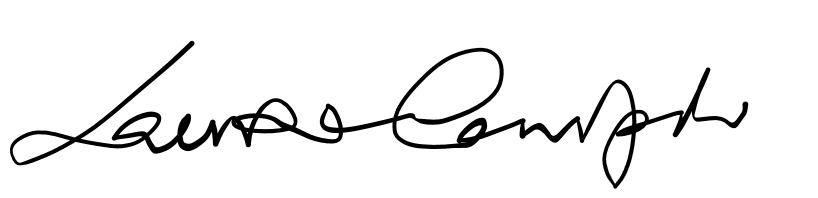
\includegraphics[width=4cm]{signature/signature0.png} \\  
\textbf{REVIEWED BY}  & Kyle Tucker             & GNC Engineer II                     & \\ 
                      & Jonte Healy             & Systems Modelling Engineer II       & \\ 
                      & Matthew Pengelly        & Lead System Modelling Engineer      & \\ 
\textbf{APPROVED BY}  & Smritee Darcy           & Optimum System Mechanical Engineer  & \\
                      & Eleazar Gonzalez-Casas  & Chief Engineer                      & \\ \hline
\end{tabular}}
\end{center}

\begin{abstract}
\noindent Jet-crossflow interaction is a critical aerodynamic phenomenon that significantly influences the stability and control of space launch vehicles and re-entry systems. This interaction occurs when a jet, such as those from reaction control system (RCS) thrusters, is injected into a high-speed external flow, resulting in complex flow structures including vortices, shock interactions, and localized pressure variations. These effects can alter the vehicle's aerodynamic characteristics and must be accurately predicted to ensure reliable flight performance and control authority. Computational Fluid Dynamics (CFD) provides a powerful tool for simulating these interactions with high spatial and temporal resolution, enabling detailed analysis of flow behavior under various flight conditions. This study investigates the dynamics of jet-crossflow interaction using CFD simulations, focusing on its impact on aerodynamic forces, moments, and overall vehicle stability. The analysis of the results highlights the importance of incorporating realistic jet modeling in CFD analyses for improved design and control of next-generation space vehicles and allowed to estimate an amplification factor for forces and moment across the flight trajectory.
\end{abstract}

%\newpage
%\makenomenclature
%\newpage
%\printnomenclature
%\section*{List of Abbreviations}
\begin{tabbing}
    \hspace{3cm} \= \hspace{8cm} \kill
    \textbf{Abbreviation} \> \textbf{Description} \\
    AEDB \> Aerodynamic DataBase  \\
    AF \> Ansys Fluent \\
    AMR \> Adaptive Mesh Refinement \\
    ARCAS \> All-Purpose Rocket for Collecting Atmospheric Soundings \\
    CAD \> Computer Aided Design \\
    CFD \> Computational Fluid Dynamics \\
    ESI \> OpenFOAM ESI Group \\
    FOs \> Functional Objects \\
    GR \> Growth Ratio \\
    GUI \> Graphical User Interface \\
    LTS \> Local Time Stepping \\
    LV \> Launch Vehicle \\
    NASA \> National Aeronautics and Space Administration \\
    OF \> OpenFOAM \\
    OS \> Operating System \\
    PIFS \> Plume-Induced Flow Separation \\
    PISO \> Pressure Implicit with Splitting of Operators \\
    SA \> Spalart Allmaras 1-Equation Turbulence Model \\
    SHM \> snappyHexMesh \\
    SIMPLE \> Semi-Implicit Method for Pressure Linked Equations \\
    SST \> Shear-Stress Transport 2-Equation Turbulence Model \\
    VSC \> Visual Studio Code \\
    WSL \> Windows Subsystem for Linux \\
    CG \> Center of Gravity \\
    CP \> Center of Pressure \\
    LE \> Leading Edge \\
    MAC \> Mean Aerodynamic Chord \\
    RK4 \> Runge-Kutta 4 Integration Method \\
    UI \> User Interface
\end{tabbing}
%
\section*{List of Symbols}
\begin{tabbing}
    \hspace{3cm} \= \hspace{9cm} \= \hspace{9cm} \kill
    \textbf{Sign} \> \textbf{Description} \> \textbf{Unit} \\
    $A$ \> Area \> m$^2$ \\
    $A_{fin}$ \> Area of one fin \> m$^2$ \\
    $A_{plan}$ \> Planform Area \> m$^2$ \\
    $A_{ref}$ \> Reference Area \> m$^2$ \\
    $A_{wet}$ \> Wetted Area \> m$^2$ \\
    $A_{aspect}$ \> Aspect Ratio of a fin, $2s / A_{fin}$ \> - \\
    $c$ \> Speed of Sound \> m/s \\
    $\bar{c}$ \> Mean Aerodynamic Chord Length of a fin \> m \\
    $c(y)$ \> Chord Length of a fin at spanwise position $y$ \> m \\
    $C_A$ \> Aerodynamic Axial Coefficient \> - \\
    $C_N$ \> Aerodynamic Normal Coefficient \> - \\
    $C_m$ \> Pitch Moment Coefficient \> - \\
    $C_{m\alpha}$ \> Pitch Moment Coefficient Derivative, $\frac{\partial C_m}{\partial \alpha}$ \> - \\
    $C_D$ \> Drag Force Coefficient \> - \\
    $C_f$ \> Skin Friction Drag Coefficient \> - \\
    $C_l$ \> Roll Moment Coefficient \> - \\
    $C_{ld}$ \> Roll Damping Moment Coefficient \> - \\
    $C_{lf}$ \> Roll Forcing Moment Coefficient \> - \\
    $D$ \> Hydraulic Diameter \> m \\
    $d$ \> Reference Length (Rocket Diameter) \> m \\
    $f_B$ \> Rocket Fineness Ratio, $L/d$ \> - \\
    $L$ \> Rocket Length \> m \\
    $m$ \> Pitch Moment \> N·m \\
    $N$ \> Normal Force or Number of Fins \> N or - \\
    $p$ \> Air Pressure \> Pa \\
    $Re$ \> Reynolds Number \> - \\
    $s$ \> Spanwise Length of One Fin \> m \\
    $T$ \> Air Temperature \> K \\
    $V$ \> Volume \> m$^3$ \\
    $v_0$ \> Free-Stream Velocity \> m/s \\
    $x$ \> Position Along the Rocket Centerline \> m \\
    $y$ \> Spanwise Position \> m \\
    $\alpha$ \> Angle of Attack \> deg \\
    $\gamma$ \> Specific Heat Ratio (for air, $\gamma = 1.4$) \> - \\
    $\Gamma_c$ \> Fin Midchord Sweep Angle \> deg \\
    $\delta_{fin}$ \> Fin Cant Angle \> deg \\
    $\eta$ \> Airflow Inclination Angle Over a Fin \> deg \\
    $\theta$ \> Roll Angle \> deg \\
    $\Lambda$ \> Dihedral Angle Fin - flow direction \> deg \\
    $\nu$ \> Kinematic Viscosity of Air \> m$^2$/s \\
    $\omega_{vel}$ \> Angular Velocity \> rad/s \\
    %$|M^2 - 1|$ \> \> - \\
    $r(x)$ \> Body or Component Radius at Position $x$ \> m \\
    $I$ \> Turbulent Intensity \> \\
    $Pr$ \> Prandtl Number \> - \\
    $U_{\infty}$ \> Free Stream Velocity \> m/s \\
    $c_p$ \> Pressure Coefficient \> - \\
    $k$ \> Turbulent Kinetic Energy \> m$^2$/s$^2$ \\
    $l$ \> Characteristic Length \> m \\
    $y^+$ \> Non-Dimensional Wall Spacing \> - \\
    $\mu_t/\mu$ \> Eddy Viscosity Ratio \> - \\
    $\kappa$ \> von Kármán Constant \> - \\
    $\omega$ \> Specific Dissipation Rate \> 1/s \\
    $\alpha_t$ \> Thermal Diffusivity \> m$^2$/s \\
    $\delta$ \> Boundary Layer Thickness \> m \\
    $\mu$ \> Dynamic Viscosity \> kg/(m $\cdot$ s) \\
    $\mu_t$ \> Turbulent Dynamic Viscosity \> kg/(m $\cdot$ s) \\
    $\rho$ \> Density \> kg/m$^3$ \\
    %$\rho_{\infty}$ \> Free Stream Density \> kg/m$^3$ \\
\end{tabbing}

\tableofcontents

%%%%%%%%%%%%%%%%%%%%%%%%%%%%%%%%%%%%%%%%%%%%%%
\section{Introduction}\label{sec:introduction}
%%%%%%%%%%%%%%%%%%%%%%%%%%%%%%%%%%%%%%%%%%%%%%
Jet-crossflow interaction refers to the complex aerodynamic phenomenon that occurs when a jet—such as those generated by reaction control system (RCS) thrusters—ejects into a high-speed external crossflow around a space vehicle. This interaction significantly alters the local flow field, creating strong vortices, shock waves, and pressure disturbances that can influence the aerodynamic forces, moments, and stability of the rocket. Understanding this interaction is critical during both atmospheric ascent and re-entry phases of a space mission, where small attitude adjustments made by the jets must be accurately predicted to ensure precise control and guidance. 

Within the scope of this work package, several tasks can be defined:

\begin{enumerate}
    \item Vernier internal flow simulation. For this batch of simulations, the simplest and crudest approximation is to assume the combustion chamber conditions to be constant with 100\% thrust at 87.5\% w/w HTP. In particular, the parameters values reported in Table~\ref{tab:vernier_inlet} should be used to initialize the Vernier internal flow simulations.
    \item Full vehicle with Vernier ON simulation
    \item Full vehicle with Vernier ON and jet ON simulation
\end{enumerate}

\begin{table}[H]
    \centering
    \caption{Thermodynamic and propellant properties.}
    \label{tab:vernier_inlet}
    \begin{tabular}{l r l}
        \toprule
        Property & Value & Units \\
        \midrule
        $P_{0c}$ (Chamber Pressure) & 64 & [bar-abs] \\
        $T_{0c}$ (Chamber Temperature) & 968 & [K] \\
        $\gamma$ (Specific Heat Ratio) & 1.267 & [-] \\
        $M_w$ (Molecular Weight) & 21.966 & [kg/kmol] \\
        $C^*$ (Characteristic Velocity) & 913.3 & [m/s] \\
        \bottomrule
    \end{tabular}
\end{table}

As for the full vehicle with Vernier ON simulation, the following scenarios may be investigated.

\begin{enumerate}
    \item Simulation at the sea level for $\alpha$ = 0$^\circ$, \textbf{jetOFF} with only 2 \textbf{VernierON} shooting perpendicularly to the orifice patch at 100\% thrust. This is to estimate the forces and moments generated and check their correctness, as the nominal values are available. In particular, jetON/VernierOFF and jetON/VernierON configuration should be compared.
    \item Simulate Max. q-$\alpha$ and/or Mach 1 trajectory points at $\alpha$ = 3$^\circ$ (or 6$^\circ$,9$^\circ$) and $\beta$ = 45$^\circ$,  \textbf{jetOFF} with only 2 \textbf{VernierON} \st{shooting at 45$^\circ$} 100\% thrust. 
    \item As it was later found, the actual Vernier thrusters shoot at about $\pm$50.3$^\circ$ w.r.t. the vertical plane, thus, also this configuration has to be assessed as potentially introducing some modifications of the flow field.
    \item The current computational domain represents only one quarter of the full geometry. Thus, a half or full body configuration may shed some light on critical issues and give a full set of actual aerodynamic coefficients.
\end{enumerate}
%
Vernier exit plane conditions for both scenarios are reported in Table~\ref{tab:vernier_plane_conditions}. It is worth noting that the Verniers do not shoot perpendicular to their surface patch but \st{approximately at an angle of 45$^\circ$ parallel to the fin they enclose}. This makes a non-negligible difference in the initialization of the numerical simulation and on the results as well. \hl{\textbf{The output to be delivered is the bending moment w.r.t. the CoM of the vehicle, the local forces exerted in the vicinity of the Verniers and globally on the vehicle to the action of the jet and the corresponding amplification factors respect to the baseline (jetOFF) configuration.}}

Figure~\ref{fig:vernier-force} shows the requirement and nominal Vernier force profiles which maps well with the provided Vernier thrust value in Table~\ref{tab:vernier_plane_conditions}. \textbf{Thus, a first check from CFD is to see if the computed force matches with this value.}

\hl{In}~\cite{rausch1973rcs} \hl{was stated that, "preliminary wind tunnel tests conducted to establish the aft RCS control effectiveness uncovered a potentially serious adverse control effect".}

\begin{table}[H]
\centering
\caption{Nozzle exit parameters for different flight states.}
\adjustbox{max width=\textwidth}{%
\begin{tabular}{lccccccc}
\toprule
\textbf{State} & \textbf{Time [s]} & \textbf{OF} & \textbf{Pc [bar]} & \textbf{ER} & \textbf{p [bar]} & \textbf{T [K]} & \textbf{v [m/s]} \\
\midrule
\rowcolor{red!10}
Throttle Down & 35.0   & 8.065 & 39.0  & 13.84 & 0.34  & 1380.6  & 2677.48 \\
MaxQ          & 39.3   & 8.137 & 28.3  & 13.63 & 0.254 & 1397.14 & 2671.51 \\
\rowcolor{red!10}
Mach1         & 60.6   & 8.17  & 25.1  & 12.83 & 0.245 & 1422.28 & 2654.32 \\
MaxQ-alpha    & 65.9   & 8.18  & 24.7  & 12.65 & 0.246 & 1428.45 & 2650.25 \\
\rowcolor{red!10}
Mach1.2       & 72.7  & 8.19 & 24.2  & 12.41 & 0.247 & 1436.33 & 2644.76 \\
Mach2         & 93    & 8.3  & 22.67 & 14.5 & 0.19   & 1395.23 & 2684.85 \\
\rowcolor{red!10}
Mach3         & 110   & 8.3  & 22.25 & 14.5 & 0.187  & 1395.41 & 2684.71 \\
Mach4         & 122   & 8.3  & 21.0  & 14.5 & 0.176  & 1395.96 & 2684.4  \\
\rowcolor{red!10}
ECO           & 136.7 & 8.28 & 20.5  & 10.50 & 0.264 & 1502.92 & 2593.7  \\
\bottomrule
\end{tabular}}
\label{tab:nozzle_exit}
\end{table}

\begin{table}[H]
    \centering
    \caption{Vernier exit parameters for different flight states.}
    \label{tab:vernier_plane_conditions}
    \adjustbox{max width=\textwidth}{%
    \begin{tabular}{llccccc}
        \toprule
        \textbf{Time [s]} & \textbf{State} & \textbf{$P_e$ [Pa]} & \textbf{$T_e$ [K]} & \textbf{$V_e$ [m/s]} & \textbf{Vernier Thrust [N]} \\
        \midrule
        \rowcolor{red!10} 0 & Liftoff & 32443 & 341 & 1495 & {1274} \\
        35 & Throttle Down & 24305.56 & 319.92 & 1520 & 1389.5 \\
        \rowcolor{red!10} 39 & Max q & 24305.56 & 319.92 & 1520 & 1414.8 \\
        60 & Mach 1 & 24305.56 & 319.92 & 1520 & 1516.3 \\
        \rowcolor{red!10} 65 & Max q-alpha & 24305.56 & 319.92 & 1520 & 1534.75 \\
        72 & Mach 1.2 & 24305.56 & 319.92 & 1520 & 1553.96 \\
        \rowcolor{red!10} 136 & ECO & 24305.56 & 319.92 & 1520 & 1606.83 \\
        \bottomrule
    \end{tabular}}
\end{table}

\begin{figure}[H]
    \centering
    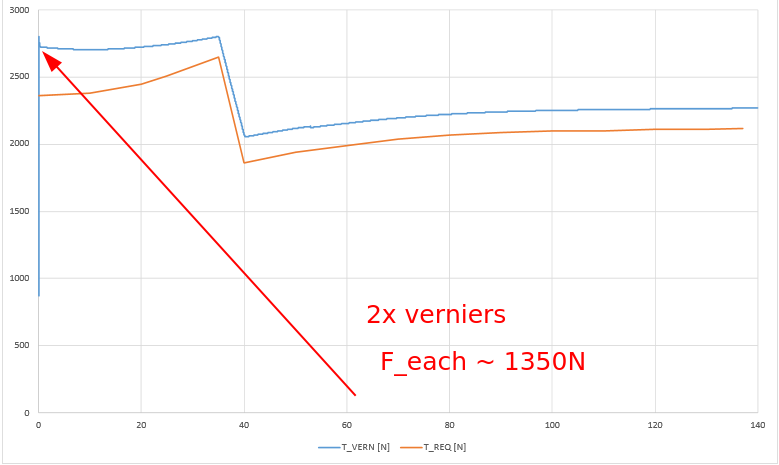
\includegraphics[width=0.6\linewidth]{figs/vernier_force.png}
    \caption{Requirement and nominal Vernier force profiles.}
    \label{fig:vernier-force}
\end{figure}

\begin{figure}[H]
    \centering 
    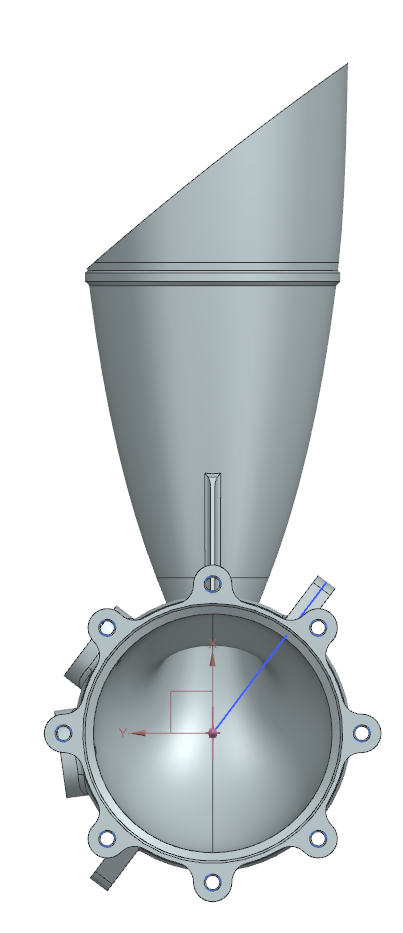
\includegraphics[angle=90,width=0.5\linewidth]{figs/v1.png}
    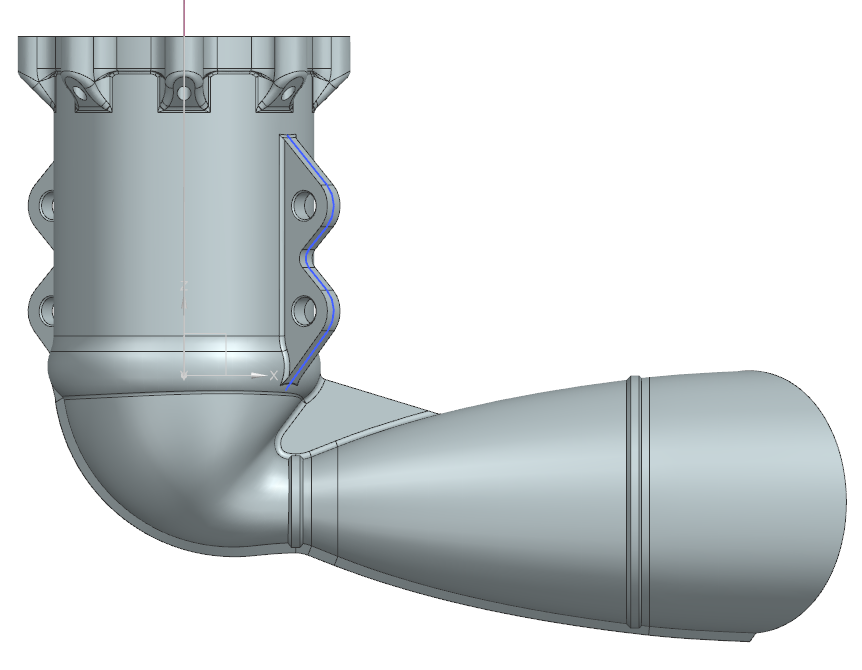
\includegraphics[width=0.495\linewidth]{figs/v2.png}
    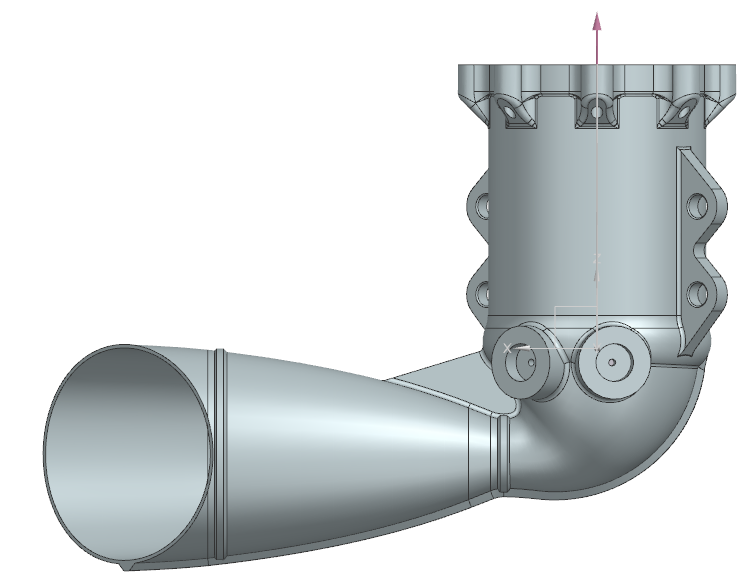
\includegraphics[width=0.495\linewidth]{figs/v3.png}
    \caption{Vernier geometry from 415-02540/415-02541 documents.}
    \label{fig:vernier-geo}
\end{figure}

\subsection{Jet Interaction with Supersonic Crossflows}
%%%%%%%%%%%%%%%%%%%%%%%%%%%%%%%%%%%%%%%%%%%%%%%%%%%%
Jet interaction with a supersonic crossflow is composed of a dominant flow interacting
with a jet flow that is typically perpendicular or near-perpendicular to the freestream
flow with a high pressure and velocity. The jet flow is perpendicular to the supersonic freestream
flow, which causes an interaction near the jet exit and additional forces applied to the
vehicle as shown in Figure~\ref{fig:1vanderWyst}.

\begin{figure}[H]
    \centering
    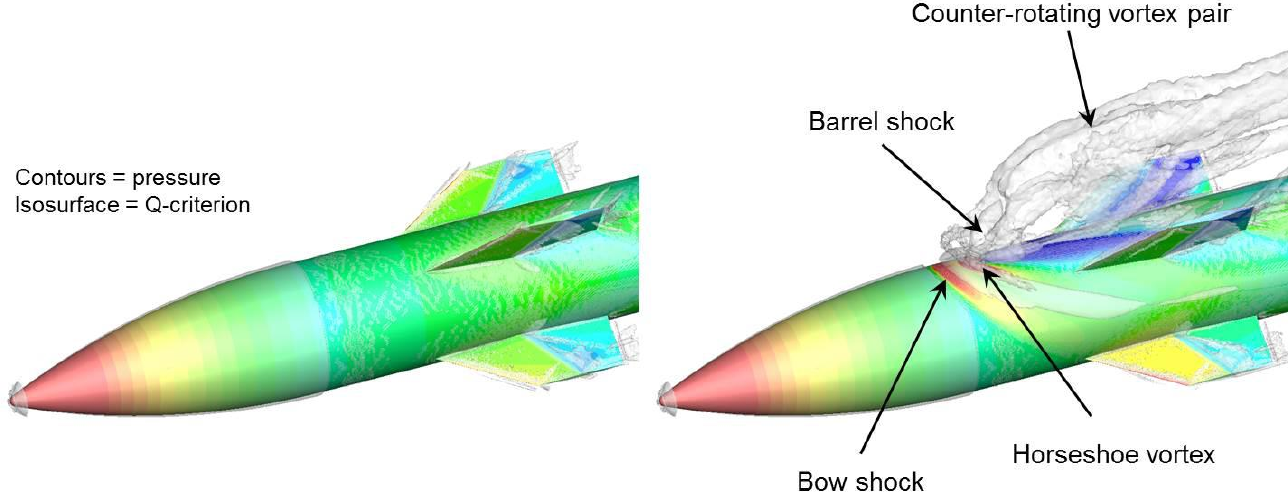
\includegraphics[width=\linewidth]{figs/fig1vanderWyst.png}
    \caption{Jet interaction for a supersonic flow on a finned vehicle flowfield with jets off or on by detached eddy simulation (DES). The fundamental jet interaction (JI) phenomenology from~\cite{vanderwyst2016computationally}, including barrel shocks and counter-rotating vortices.}
    \label{fig:1vanderWyst}
\end{figure}

There is a flow discontinuity that must be resolved due to the different flow conditions between the jet and freestream. This usually results in boundary layer separation and vortex shedding around the jet exit in subsonic and supersonic flight regimes. In supersonic flow, there are shock waves and expansion waves that form as a result of the freestream flow diverting around the jet flow. This combination of compressibility and turbulence leads to a complex interaction that is difficult to predict based on the flow and jet conditions. Experiments or high-fidelity computations are needed that capture all of these JI effects to analyze resulting flow structure and the net force applied to the vehicle. A diagram of the main JI flow structures is shown in Figure~\ref{fig:spand1968}. % and a snapshot from a dynamic computational result is shown in Figure~\ref{fig:kawai} with the flow shocks, boundary layer, and vorticity.

\begin{figure}[H]
    \centering
    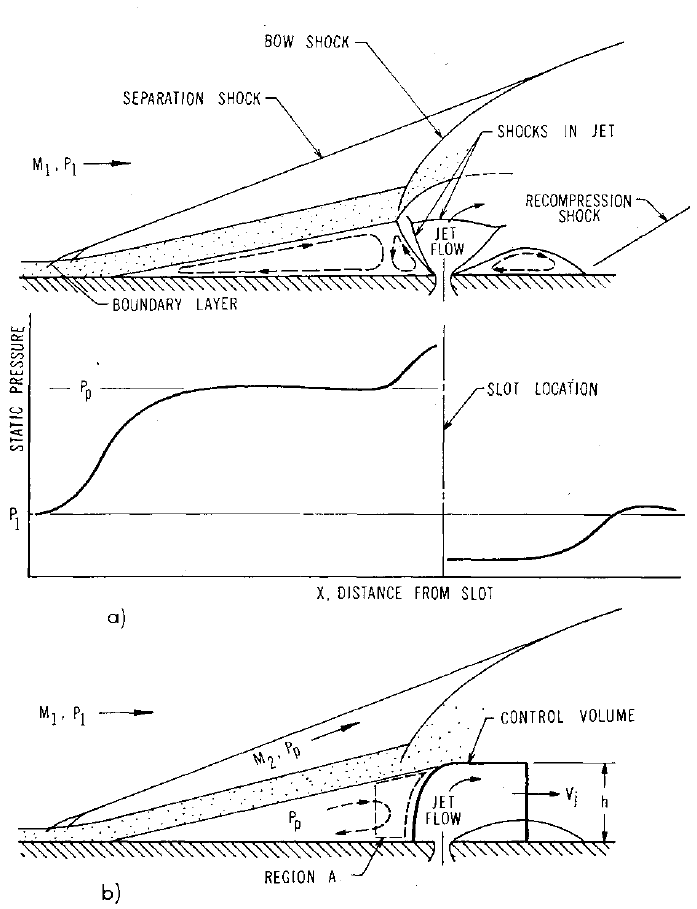
\includegraphics[width=0.9\linewidth]{figs/fig1spand1968.png}
    \caption{Diagram by Spaid and Zukoski~\cite{spaid1968study} of jet interaction with supersonic crossflow highlighting the main flow structures.}
    \label{fig:spand1968}
\end{figure}

A disadvantage of lateral control jets, however, is the complex flow pattern to control as
it is shown in Figure~\ref{fig:seiler2003} reproduced from~\cite{Seiler2003}. 

\begin{figure}[H]
    \centering
    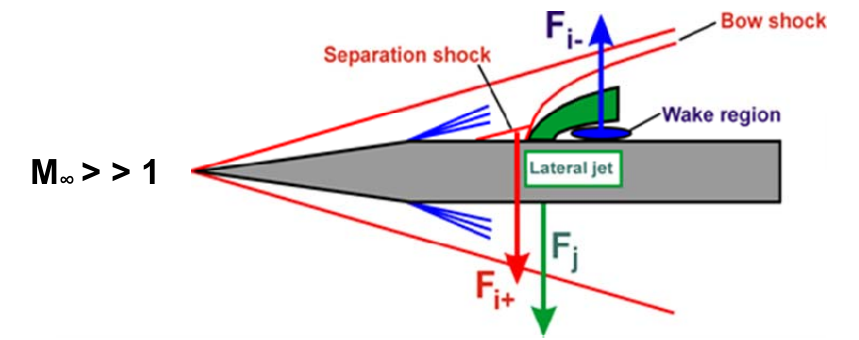
\includegraphics[width=\linewidth]{figs/fg2.png}
    \caption{Flowfield around a missile geometry in the presence of lateral control jet by Seiler et al.~\cite{Seiler2003}.}
    \label{fig:seiler2003}
\end{figure}

In terms of performance of the technique two main aspects are worth noting; firstly low-pressure region behind the jet effectively creates suction. Even though the amount of suction is moderate it acts over a large area aft of the injector thus creating a strong upward force. The second, and in many aspects most detrimental effect is the coupling with the high pressure region ahead of the jet and the formation of a nose down moment about the injector. The contribution to the nose down moment from the low pressure region can be particularly high since this region sustains far aft of the injector. %This shift in the center of pressure of the vehicle has to be corrected through the use of an attitude control system that actuates counterbalancing jet thrusters [34]. 

\hl{The important performance parameters are; i) the \textbf{thrust ratio}, which is the ratio of the side force to axial thrust force, ii) \textbf{amplification}, which is the ratio of side specific impulse $I_{sp_s}$ to main axial specific impulse $I_{sp_s}$ and it determines the amount of fluid to be injected to have a specified side force, and iii) \textbf{axial thrust augmentation}, is the ratio of the augmented axial impulse $\Delta I_{sp_p}$ to main specific axial impulse and is a measure of the penalty of the overall system to obtain this side force}.

The detailed averaged flow features of two dimensional transverse jets in supersonic crossflows over a flat plate are shown in Figure~\ref{fig:1.6}. The secondary jet basically acts as an obstruction on the main flow, diverting it to move above the injection plume. This blockage projects itself by a strong jet induced bow shock upstream in the inviscid region. Consequently due to the presence of this bow shock an adverse pressure gradient is imposed on the incoming turbulent boundary layer; causing it to separate upstream. The flow structure in the turbulent boundary
layer involves two counter rotating vortices, primary upstream vortex (PUV) and secondary upstream vortex (SUV). These structures provide a region where the boundary layer and jet fluids mix subsonically upstream of the jet exit. The size of the separation region is bigger for laminar boundary layer due to its less energetic nature, hence less resistant to adverse pressure gradients. The boundary layer displacement of upstream vortices causes a weak separation shock that interacts with the strong bow shock. In between the recirculation region and separation shock there is a sonic surface which essentially displaces the incoming flow. On the injection port the under-expanded sonic transverse jet suddenly accelerates and expands into the main flow and results reduced pressures. This expansion is ended by a normal shock; resulting a Mach surface surrounding the jet plume. 

\begin{figure}[H]
    \centering
    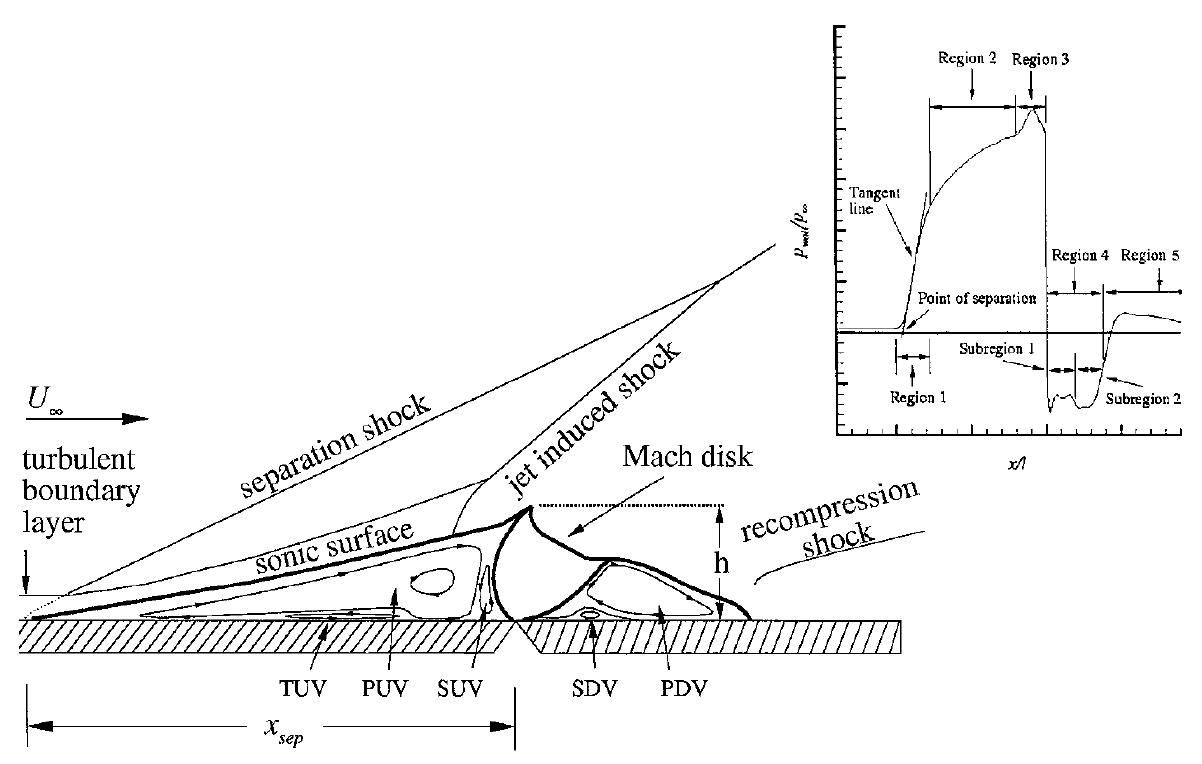
\includegraphics[width=\linewidth]{figs/fg1.6.png}
    \caption{Two dimensional transverse slot injection flow field features by Spaid and Zukoski~\cite{spaid1968study}.}
    \label{fig:1.6}
\end{figure}

\textbf{Penetration} of the jet was shown to be dependent primarily on the jet to free stream \textbf{momentum flux ratio}, J, as mentioned in Equation~\ref{eq:J}:

\begin{equation}
    J = \frac{\gamma_{\text{jet}} \, p_{\text{jet}} \, M_{\text{jet}}^2}{\gamma_\infty \, p_\infty \, M_\infty^2}
    \label{eq:J}
\end{equation}

At the downstream of the injection location the diverted main flow is turned parallel to the nozzle wall via a recompression shock accompanied by a recirculation region forming primary and secondary downstream vortices (PDV and SDV). A third upstream vortex (TUV) might occur occasionally. In the wall static pressure profile, Figure~\ref{fig:1.6} there are five distinct regions reported by Spaid~\cite{spaid1968study}; an upstream region of steep pressure rise (region 1) as a result of boundary-layer separation, then a flattening of the pressure upstream of the jet (region 2) caused by PUV. The pressure plateau is followed by a pressure spike (region 3) caused by the SUV. Immediately downstream of the jet is a large pressure drop (region 4) with two subregions. The first subregion is a slight pressure rise caused by the leading edge of the PDV. The second subregion is a pressure drop caused by the SDV. The pressure drop is followed by a pressure hump (region 5) associated with the trailing edge of the PDV, boundary-layer reattachment, and the recompression shock. For laminar interactions the pressure plateau is more gradual and the pressure spike is smaller. In case of a transverse injection through a single circular hole into a cross flow, namely three dimensional jet interaction, significant fluid motion in span wise direction is observed additionally. Two counter rotating vortices, emerging on top of Mach disc and a horseshoe vortex, formed by the SUV, wrap around the upstream side of the jet and propagate downstream; moreover the bow shock is curved in spanwise direction as well and the main flow is diverted both above and on the sides of the injection port~\cite{Gruber1995} as shown in Figure~\ref{fig:1.7}.

\begin{figure}[H]
    \centering
    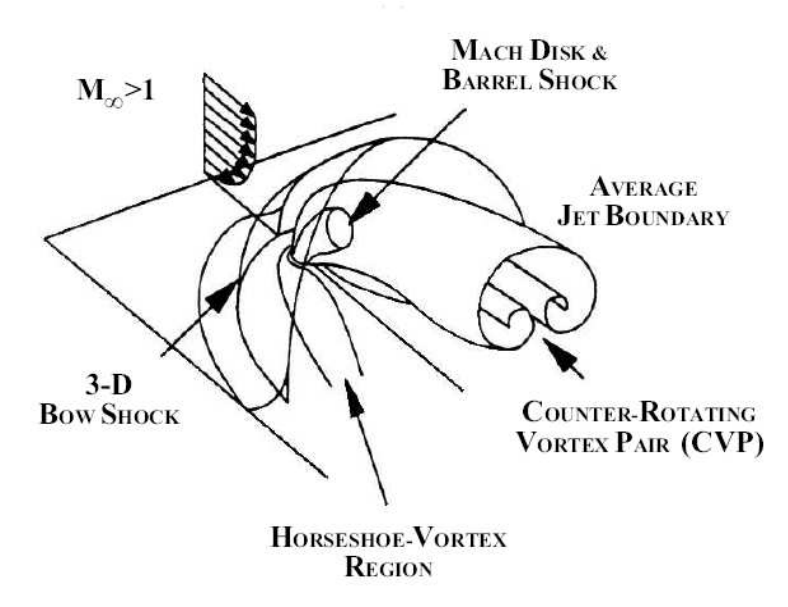
\includegraphics[width=\linewidth]{figs/fg1.7.png}
    \caption{3D perspective of the averaged features of the flowfield by Gruber~\cite{Gruber1995}.}
    \label{fig:1.7}
\end{figure}

This pair of counter rotating cross flow vortices is assessed by~\cite{santiago1995velocity} as the primary source of entrainment of the surrounding incoming flow air into the injectant’s flow that is important for farfield mixing. These structures are produced by folding of the vortex ring, which is a downstream manifestation of the vorticity arising from the injectors sidewall boundary layers. Haven and Kurosaka~\cite{haven1996improved} demonstrated that the injector geometry has a strong influence on the near field character of the these vortices. The jet shear layer vortices on the windward boundary of the jet are stemming from Kelvin-Helmholtz instabilities due to the significant shear layer formed between the low speed fluid behind the bow shock and the high speed jet. The horseshoe vortices wrap around the upstream side of the jet and trail downstream; wake vortices periodically shed near the base of the inner jet core and trail downstream under the jet plume.

In terms of pressure distribution, the three dimensional relieving effect assists the main flow to move around the transverse jet, which reduces maximum value of the surface static pressure and it causes upstream separation point move closer to the jet. Hence the extent the affected area due to the transverse jet is reduced as well as the magnitude of the pressure peak for the same $J$ value. At the same time, higher pressures that are observed near the interaction shocks, which are wrapped around the plume, are augmenting the interaction force component generated in this region. Whether the net effect is an addition or subtraction, for a finite span plate, it is likely to depend on all of the parameters that affect the interaction. %The effects of finite span jet nozzles on interaction phenomena is shown in Figure~\ref{fig:1.8}.

%\begin{figure}[H]
%    \centering
%    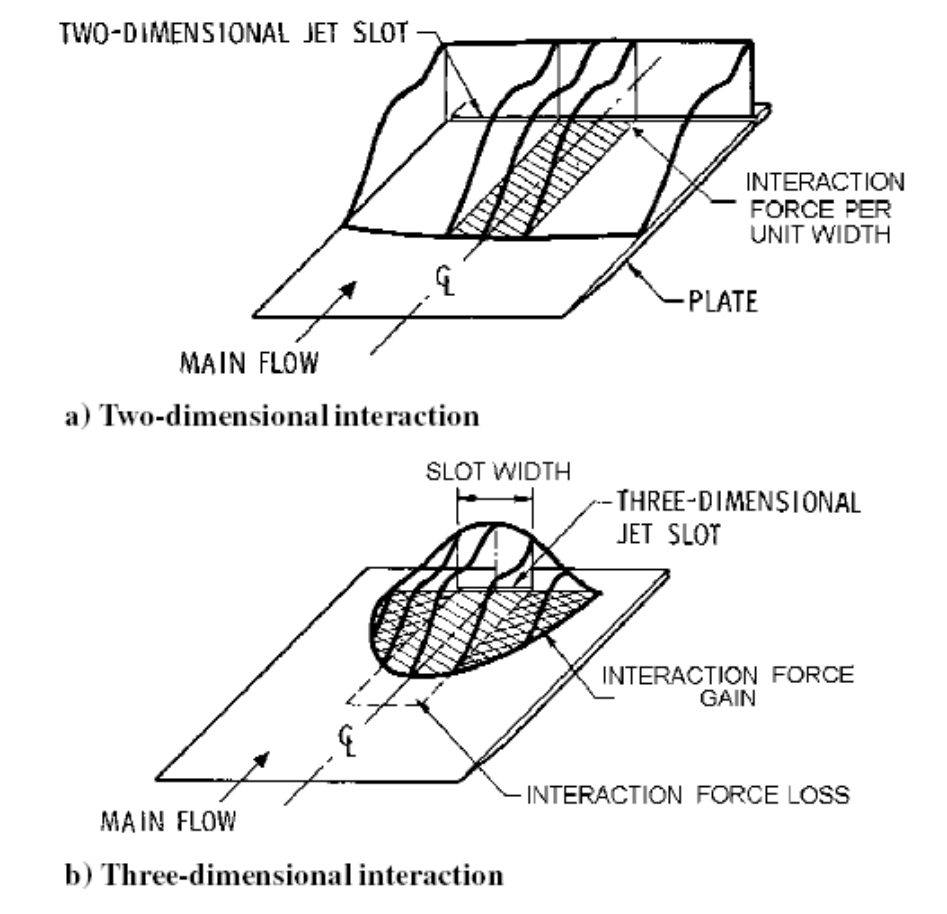
\includegraphics[width=\linewidth]{figs/fg1.8.png}
%    \caption{Effects of finite span nozzles in jet in uniform cross flow by Cassell~\cite{cassel2003applying}.}
%    \label{fig:1.8}
%\end{figure}

%\begin{figure}[H]
%    \centering
%    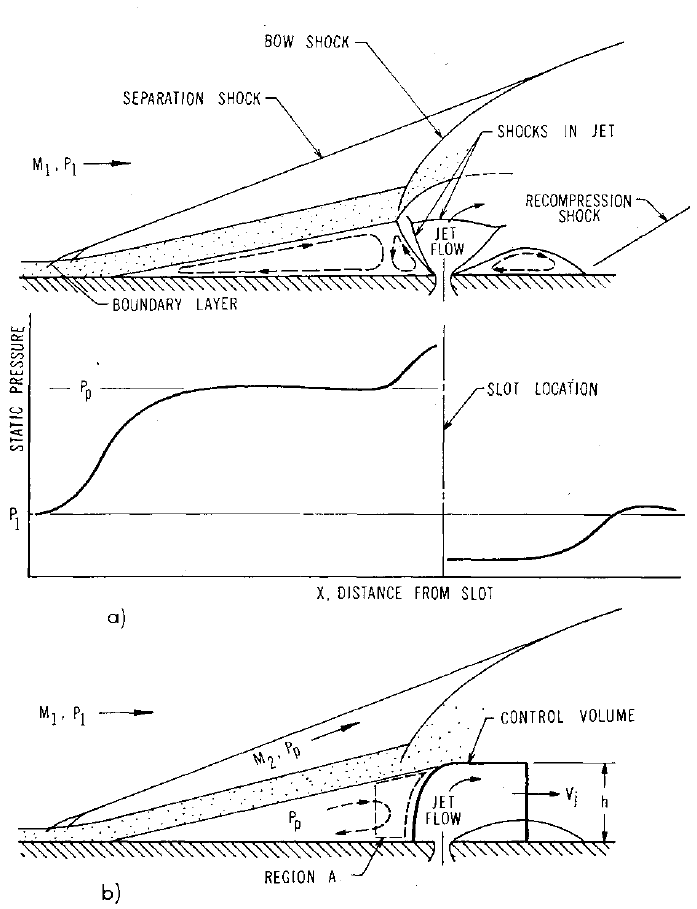
\includegraphics[width=\linewidth]{figs/fig1spand1968.png}
%    \caption{Diagram by Spaid and Zukoski~\cite{spaid1968study} of jet interaction with supersonic %crossflow highlighting the main flow structures.}
%    \label{fig:spand1968}
%\end{figure}

%\begin{figure}[H]
%    \centering
%    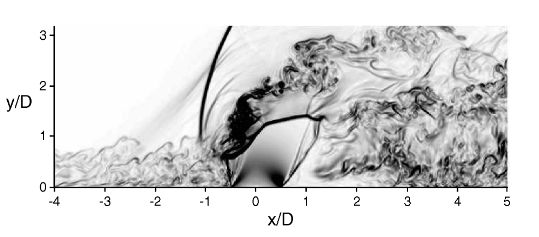
\includegraphics[width=\linewidth]{figs/fig1.8.png}
%    \caption{Large eddy simulation results by Kawai and Lele~\cite{kawai2010large} of the density %gradient magnitude from jet interaction with supersonic crossflow showing the flow structures %including shocks and vortex shedding.}
%    \label{fig:kawai}
%\end{figure}

Previous experimental studies have been conducted regarding the JI with a supersonic crossflow and the characteristic steady-state flow condition has been well documented. Spaid and Zukoski~\cite{spaid1968study}, Spaid and Cassel~\cite{spaid1973aerodynamic}, and Zukoski and Spaid~\cite{zukoski1964secondary} experimentally identify the flow structure and developed preliminary models for the interaction. These results also identify the potential increase in jet control authority due to the supersonic flow interaction, which could be leveraged to improve vehicle maneuverability.

Roger~\cite{roger1999aerodynamics} summarizes the JI literature of the previous 50 years, collected the common trends and critical parameters, and highlighted the remaining challenges. One
of the challenges was the sporadic approach to the problem throughout the literature
and a lack of a common methodology that could be used for multiple vehicles, flight
conditions, and jet conditions. Another important issue noted by Roger~\cite{roger1999aerodynamics} is the "jet-on jet-off transients issue", which refers to the fluid dynamic response as a result of pulsed or throttled jet flow. %This summary motivates further research that compares multiple vehicle configurations with more emphasis placed on the jet interaction transient response.

\subsection{Analytical and Empirical Modeling}
%%%%%%%%%%%%%%%%%%%%%%%%%%%%%%%%%%%%%%%%%%%%%%
Previous work on modeling JI with a supersonic crossflow extends back before computing resources were advanced enough to tackle the problem. Various empirical and theoretical modeling efforts have been made to correlate the flow and jet conditions to the flow velocity or surface quantities~\cite{billig1971unified,werle1972jet,young1972viscous,demuren1994modeling}.

Early experimental results yielded a \textbf{scaling parameter} that is presented by Zukoski
and Spaid~\cite{zukoski1964secondary}. \ul{This scaling parameter could be used to correlate the jet penetration height into the flow and jet parameters}. Experimental results show very good correlation with the scaling parameter and the work is extended to calculate a similar scaling parameter for the total force on the wall. Then, Spaid and Zukoski~\cite{spaid1968study} develop an analytic model based on the characteristic structure of the JI experimental results. The analytic model involved creating a control volume for the jet flow to then calculate useful quantities such as the pressure upstream of the jet as well as the jet penetration height into the flow and amplification factor.

\textbf{The amplification factor is a useful quantity to measure the relative effect of the JI to the jet thrust} and it has been used throughout the JI literature~\cite{spaid1968study,spaid1973aerodynamic,roger1999aerodynamics,margason1993fifty}. The \hl{jet amplification factor K} for quantity F is calculated as in Equation~\ref{eq:Kfac}:

\begin{equation}
    K_F = \frac{F_j + F_{ji}}{F_j}
    \label{eq:Kfac}
\end{equation}

where $F_j$ corresponds to the contribution from the jet thrust alone, $F_{ji}$ is the contribution of the interaction with the external flow. \textbf{An amplification factor greater than 1 indicates that the loads due to jet interaction amplifies the net forces and moments, less than 1 indicates a reduction in the net forces and moments, and less than 0 indicates control reversal.} This quantity is used to quantify the jet interaction effect on the vehicle model.

Later results are tied to more complex flow quantities of interest, such as Young~\cite{young1972viscous} that presents a solution procedure to calculate the \textbf{boundary layer separation distance} and amplification factor. These amplification factor results compare well to previous experiments including Spaid and Zukoski~\cite{spaid1968study}. The whole two-dimensional JI flow structure can be modeled following Werle, Driftmyer and Shaffer~\cite{werle1972jet} using a series of flat plate experiments. The model presented by Werle, Driftmyer and Shaffer~\cite{werle1972jet} calculates the surface pressure distribution due to the characteristic JI features such as boundary layer separation, normal shock, flow turning, and re-compression shock by relating the various flow and jet parameters.

The previously discussed results are primarily focused on the flat plate results and
the longitudinal jet plane, which neglects the three-dimensional effects. zroadwell~\cite{broadwell1963analysis} includes the three-dimensional effects by considering JI and the resulting shock formation similar to the propagation of a blast wave due to a high energy explosion. The blast wave propagation in air had been developed previously by Taylor~\cite{taylor1950formation} and Sakurai~\cite{sakurai1953propagation,sakurai1954propagation} for intense explosions. Broadwell~\cite{broadwell1963analysis} then considers the blast wave to propagate with the free-stream flow to calculate shock wave propagation downstream between the jet flow and free-stream flow. The model developed by Broadwell~\cite{broadwell1963analysis} compares well with experiments when calculating the total force applied to the plate by the JI.

Overall, the previous work in JI analytic modeling has been shown to correlate well with experimental results for integrated quantities or two-dimensional pressure distributions, but a three-dimensional analytic model would still be needed when considering more complex geometries and varied flow conditions.

\subsection{Computational Modeling}
%%%%%%%%%%%%%%%%%%%%%%%%%%%%%%%%%%%
Detailed computational modeling has the ability to simulate the JI problem for complex geometry, flow and jet conditions~\cite{warfield1989calculation,graham1999numerical,sahu2024,amick1963experimental,despirito2011factors,despirito2012lateral,despirito2014predictions,despirito2012transient,despirito2015turbulence,gnemmi2008computational}. Cassel~\cite{cassel2003applying}, Demuren~\cite{demuren1994modeling} and Margason~\cite{margason1993fifty} review the numerical modeling approaches and results that focus on solving the governing equations for the jet-in-crossflow problem.

Cassel~\cite{cassel2003applying} summarizes the computational literature on JI with supersonic crossflow along with experimental and flight test results. It was noted that JI analysis using
computational methods introduces additional complexity such as turbulence modeling, mesh refinement, and shock-capturing that are critical to the solution. Vehicle simulation models including jet interaction must be sensitive to these compressible and turbulent effects in the flow to accurately model the resultant loads. Warfield~\cite{warfield1989calculation} compares the numerical simulation results to experiments and noticed that \textbf{the turbulence model had a significant effect on the predicted flow separation region}. DeSpirito~\cite{despirito2015turbulence,despirito2011factors} investigates this turbulence modeling issue further by comparing several available models to experimental results for flat plate experiments and axisymmetric vehicles for varying flow and jet conditions. The numerical results of demonstrate the \textbf{wide variance between turbulence models in the ability predict the separated flow around the jet nozzle exit}. In addition, \textbf{there was not a consistently accurate model across all test cases}, which adds to the complexity of JI numerical modeling.

Several research studies~\cite{ferrante2010inclined,ziefle2009large,kawai2010large} have used a Large Eddy Simulation (LES) approach to more accurately model the turbulence in the flow and capture the vortex shedding, shear layer and barrel shock among other JI features. Despite capturing these effects, one major conclusion was that \textbf{the turbulence level of the inflow conditions had a significant impact on the solution}. The computational studies of JI have shown that it is possible to match the experimental conditions, but \textbf{it is difficult to know what computational method is suitable a priori}. In addition, these methods are computationally expensive and would be prohibitive for studying early design iterations of a vehicle. Computational modeling also highlights important phenomena such as the jet transient  forces~\cite{Ebrahimi2000,Naumann1998,despirito2012transient}. It is critical to understand the dynamics of the JI with varying flow and jet conditions considering a maneuverable vehicle in a dynamic flight environment. 

Some experimental and computational work has focused on the transient issue of firing a jet into a supersonic crossflow. Randolph, Chew, and Johari~\cite{Randolph1994} fired a pulsating jet into a crossflow and noted a significant difference in the penetration of the jet into the crossflow to improve mixing in combustion applications. Experimental results by Naumann et al.~\cite{Naumann1998} show significant oscillation in the applied forces due to the JI effect, which would become critical to model during vehicle maneuvers with varying jet thrust. Ebrahimi~\cite{Ebrahimi2000} also presents the oscillation and variation of the resultant JI forces and moments due to turning the jet on and off with a characteristic time to develop the steady state on the order of milliseconds. LES results of the supersonic JI problem by Genin and Menon~\cite{Génin01012010} show \textbf{unsteadiness in the flow field itself with large-scale vortices from the windward side of the jet leading to significant deviations from the time-averaged flow}. DeSpirito ~\cite{despirito2012transient} examines the transient behavior of the JI with a full vehicle model and the results show that \textbf{the integrated forces reach the steady-state value before the pressure distribution}. This effect can be neglected for rigid flight vehicles, but the pressure distribution is critical to calculating the structural response. These transient results in combination with the findings by Roger~\cite{roger1999aerodynamics} emphasize the need for more understanding of the jet interaction dynamics as wells as modeling methods for these effects.

The transient jet interaction effects on vehicle flight response are observed in computational work by Sahu, Fresconi, and Heavey~\cite{sahu2024}. Flight simulations of a rigid projectile with control jets are completed with a coupled CFD and rigid-body dynamics model. The total angle of attack is below 20 degrees at Mach 2, the pulsed time is short (2-20 ms) and the total flight time was limited to one second. The jet was fired once with varying initial angular rates and showed the control authority to divert the projectile from its path. An aerodynamic and jet interaction model is developed by Sahu et al.~\cite{sahu2024} that compared favorably to the coupled CFD/Rigid-Body Dynamics (RBD) flight simulation results. The authors conclude that \textbf{the JI had a significant effect on the projectile trajectory} and further study would be required to ensure the accuracy of the projectile.\textbf{ However, the jet effects are incorporated using the integrated force and moment amplification factors, which does not directly include the pressure distribution due to jet interaction}. The pressure distribution would be required for aeroelastic analysis to model the correct load distribution and resulting structural deformation.

Previous research regarding the JI with a supersonic crossflow for high-speed vehicles has demonstrated a variety of trends enabled by numerical simulation using CFD. DeSpirito~\cite{despirito2011factors} and Graham and Weinacht~\cite{graham1999numerical} used computational modeling to investigate a wide variety of vehicle design choices such as surface geometry, jet location, and jet nozzle-exit-to-throat ratio. The numerical results by DeSpirito~\cite{despirito2012lateral} of the lateral JI with the Army-Navy Basic Finner model demonstrate how \textbf{the total applied force is strongly dependent on the jet location as well as the proximity to the fins}. Cassel~\cite{cassel2003applying} alludes to this in a review of JI technology as well. Therefore, \textbf{the prevailing wisdom has been to place the attitude control jets at the tail end of the vehicle to remove the low-pressure expansion region from the vehicle surface, maintain the high pressure region, and maximize the applied moment to the vehicle}. Computational analysis continues to further the understanding of JI, but the computational cost increases and robustness decreases as the modeling methods become more complex. The majority of JI analysis has focused on steady-state flow and jet conditions with a rigid vehicle. Additional considerations are required for the vehicle control applications such as the intermittent pulsing of the jet, the vehicle attitude, and vehicle dynamics that all affect the flow and resulting JI. In addition, slender high speed vehicles have added flexibility that will lead to FSI due to larger structural deformations under large aerodynamic loads. 

These results and intuition have been developed with rigid vehicle models or considering each physical domain separately. A vehicle model that includes structural degrees of freedom in addition to the JI effect is needed to fully understand the impact on slender vehicle performance and stability with attitude control jets. If the attitude control jet was placed at the tail of the vehicle, then the applied moment would cause a structural deformation that decreases the control effectiveness. However, if the attitude control jet is located near the nose of the vehicle the attitude jet would cause a favorable structural deformation. If the jet location is intelligently chosen, then the high and low pressure regions of the JI could both have a favorable impact on the vehicle deformation that mitigate the loss in effectiveness due to the low pressure region.

% https://tex.stackexchange.com/questions/19579/horizontal-line-spanning-the-entire-document-in-latex
%\noindent\makebox[\linewidth]{\rule{0.75\paperwidth}{0.4pt}}

%%%%%%%%%%%%%%%%%%%%%%%%%%%%%%%%%%%%%%%%%%%%%%%%%%%%%%%%%%%%%%%%%%%%%%%%%%%%%%%%%%%%%%%%%
Before discussing results, it will be instructive to offer a brief description of the jet interaction phenomena and its effects. First consider a simple flat plate with a transverse jet firing upward, as sketched in Figures~\ref{fig:jet2d0}-\ref{fig:jet2d3d}. This type of configuration is generally classified as "classical" jet interaction. The plume acts like a step, or barrier, to the flow and induces the boundary layer upstream of the plume to separate. A separation shock originates at the separation point. Because of the boundary-layer separation the static pressure upstream of the jet rises to $P_2$ and then, because of the counter-rotating vortices, jumps again to $P_{2'}$ in the immediate vicinity of the jet. Immediately downstream of the jet is a second separated region designated by the pressure $P_3$. For supersonic flow, $P_3$ is less than the initial pressure $P_1$. However, if the external flow is hypersonic, the downstream pressure $P_3$ is often greater than $P_1$. A recompression shock downstream of the separated region turns the flow parallel to the wall and raises the static pressure to $P_4$. 

The Charon flowfield, of course, is much more complex, and the "classical" jet interaction effects are significant only for the aft jets firing transversely. In addition, there is some interaction of the plume with the flowfield over the top of the fins which may create a significant interaction in roll. A left-hand yaw jet, by virtue of its location above the center of gravity, will induce a positive rolling moment. The jet interaction effects are strong enough in some instances to not only reduce this positive rolling moment but reverse it. Classical jet interaction plays a part in the effectiveness of the up- and down-firing RCS jets, these jets also have a significant effect on nearby vehicle surfaces through plume interaction with the boundary layer and plume impingement to the surface itself.

%The down-firing jets, although canted outboard and aft of the vehicle, impinge heavily on the fin (mostly trailing) edge. There is also a significant amount of jet interaction independent of plume impingement. These interactions (both impingement and jet interaction) induce a, strong pitch-up moment and, for a left-hand jet, a left-wing-down rolling moment and a nose-right yawing moment.

%The up-firing jets provide considerable interaction with the vertical tail. Since this jet is operated in a flight regime where the angle of attack is quite high (a « 40 deg) and the tail is in separated flow, most of the plume interaction with the vertical tail is due to plume impingement which produces sizable—and opposing—interaction moments in roll and yaw. A minimal amount of pitching moment is induced because there is very little jet interaction between the jet and the flow over the top of the OMS pods

\begin{figure}[H]
    \centering
    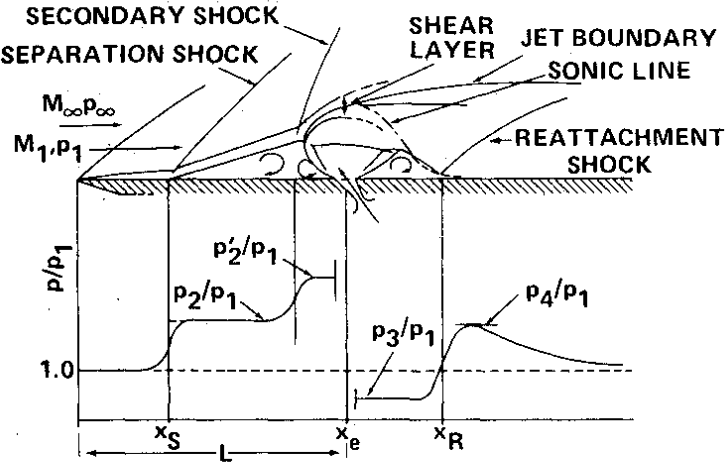
\includegraphics[width=0.9\linewidth]{figs/Screenshot from 2025-06-24 13-30-27.png}
    \caption{Two-dimensional jet interaction phenomenology.}
    \label{fig:jet2d0}
\end{figure}

\begin{figure}[H]
    \centering
    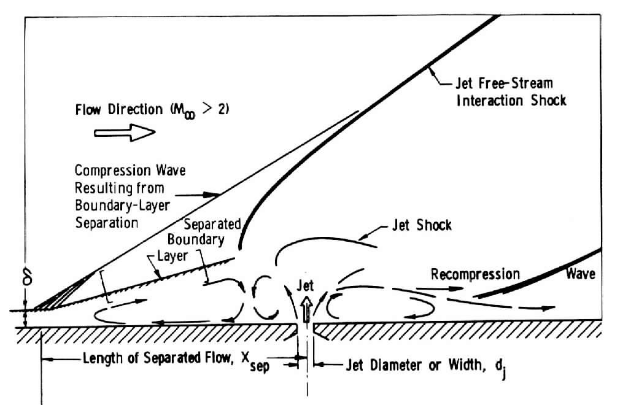
\includegraphics[width=\linewidth]{figs/Screenshot from 2025-06-26 09-59-14.png}
    \caption{Two-dimensional jet interaction phenomenology.}
    \label{fig:jet2d}
\end{figure}

\begin{figure}[H]
    \centering
    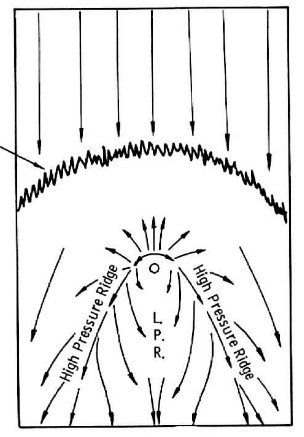
\includegraphics[width=0.4\linewidth]{figs/Screenshot from 2025-06-26 09-59-36.png}
    \caption{Two-dimensional jet interaction phenomenology.}
    \label{fig:jet2d}
\end{figure}

\begin{figure}[H]
    \centering
    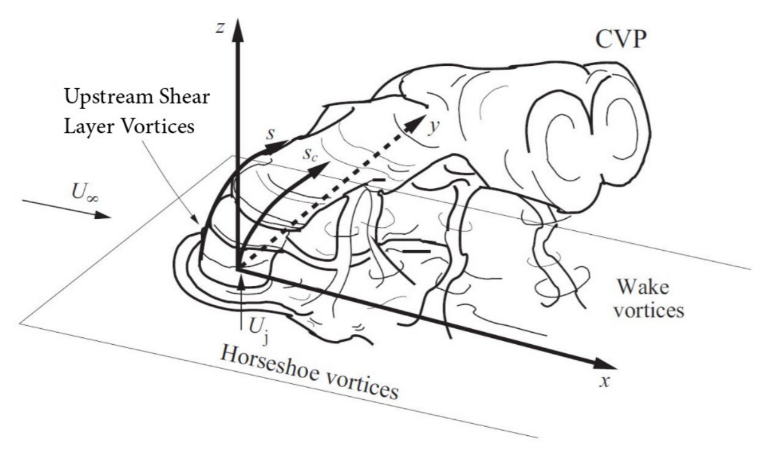
\includegraphics[width=0.8\linewidth]{figs/Screenshot from 2025-06-26 10-14-03.png}
    \caption{A representative depiction of the JICF, where dominant vortex systems are shown, including the horseshoe vortex which wraps around the leading edge of the jet column and extends downstream, the shear layer vortices which form on the upstream side of the jet near the jet exit plane and convect along the shear layer, the upright wake vortices further downstream which entrain wall boundary layer fluid into the jet, and the counter-rotating vortex pair (CVP), which is the most dominant flow feature associated with jet cross-section. Characterization of the flowfield is typically made with nondimensional parameters such as the \textbf{jet-to-crossflow velocity ratio} ($R = U_j /U_{\infty}$), jet-to-crossflow density ratio ($S = \rho_j/\rho_{\infty}$), \textbf{jet-to-crossflow momentum flux ratio} ($J = \rho_j U_j^2/\rho_{\infty} U_{\infty}^2 = SR^2$), and jet Reynolds number ($Re_j = \rho_j U_j D/\mu_j$), which is based on the jet exit diameter (D), bulk (spatially averaged) jet velocity ($U_j$), and jet absolute viscosity ($\mu_j$).}
    \label{fig:descr}
\end{figure}

\begin{figure}[H]
    \centering
    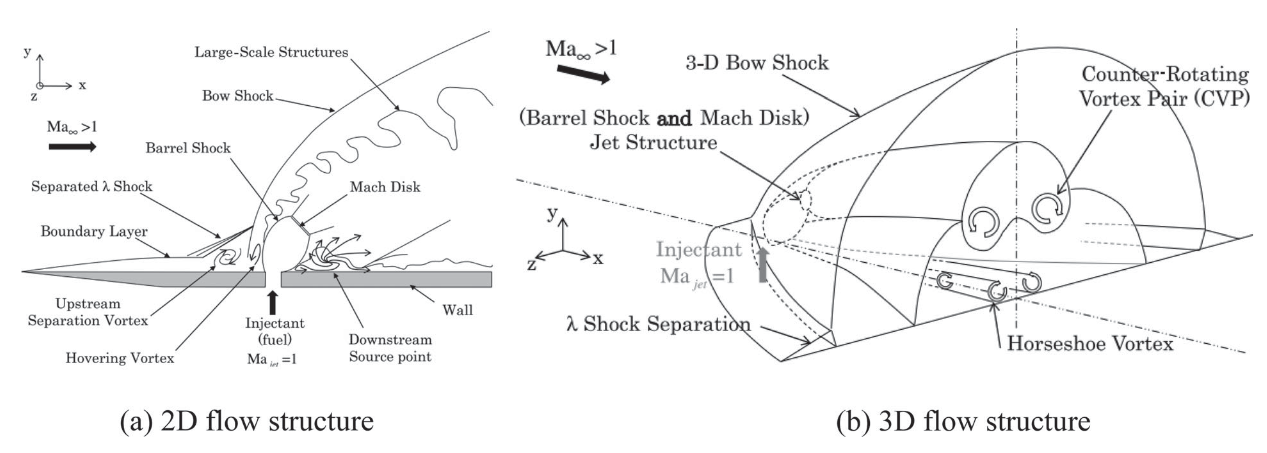
\includegraphics[width=\linewidth]{figs/Screenshot from 2025-06-26 10-16-26.png}
    \caption{Typical structures of (a) 2D and (b) 3D jet injection into supersonic flow~\cite{hill2004hybrid}. Main flow structures such as three-dimensional (3D) bow shock (BoS), upstream recirculation zone (RZ), and horseshoe vortices are generated due to the blockage effect of the jet. Under the action of the crossflow, the counter-rotating vortex pair; shock wave jet flow expands obliquely along the mainstream and is compressed by the Mach disk (MD). The jet shear layer develops into a large-scale streamwise counter-rotating vortex pair (CVP), which is believed to dominate the vortex structure and mixing process behind the jet. Several small CVPs, wake shock waves, and few downstream RZs appear behind the jet.}
    \label{fig:jet2d3d}
\end{figure}

%%%%%%%%%%%%%%%%%%%%%%%%%%%%%%%%%%
\section{Method}\label{sec:method}
%%%%%%%%%%%%%%%%%%%%%%%%%%%%%%%%%%
ANSYS Fluent computes aerodynamic forces, moments, and their dimensionless coefficients using surface integrals of pressure and viscous stress over specified wall zones. 

\subsection{Force Calculation}
%%%%%%%%%%%%%%%%%%%%%%%%%%%%%%
The total force acting on a wall zone is obtained by integrating pressure and viscous stresses:

$$
\vec{F} = \int_{A} \left( -p \vec{n} + \vec{\tau} \right) dA
$$

where:
   
- $ p $: static pressure
    
- $ \vec{n} $: unit normal vector to the surface
    
- $ \vec{\tau} $: viscous stress vector
    
- $ A $: surface area of the selected wall(s)


\subsection{Moment Calculation}
%%%%%%%%%%%%%%%%%%%%%%%%%%%%%%%
The aerodynamic moment about a reference point $\vec{r}_0$ is given by:

$$
\vec{M} = \int_{A} \left( \vec{r} - \vec{r}_0 \right) \times \left( -p \vec{n} + \vec{\tau} \right) dA
$$

where:
    
- $ \vec{r} $: position vector of the surface element
    
- $ \vec{r}_0 $: moment reference point

\subsection{Dimensionless Aerodynamic Coefficients}
%%%%%%%%%%%%%%%%%%%%%%%%%%%%%%%%%%%%%%%%%%%%%%%%%%%
Fluent uses dynamic pressure $ q_\infty = \frac{1}{2} \rho_\infty V_\infty^2 $ to compute non-dimensional coefficients:

\subsubsection*{Drag Coefficient}
%%%%%%%%%%%%%%%%%%%%%%%%%%%%%%%%%

$$
C_D = \frac{F_D}{q_\infty S}
$$

\subsubsection*{Lift Coefficient}
%%%%%%%%%%%%%%%%%%%%%%%%%%%%%%%%%

$$
C_L = \frac{F_L}{q_\infty S}
$$

\subsubsection*{Side Force Coefficient}
%%%%%%%%%%%%%%%%%%%%%%%%%%%%%%%%%%%%%%%

$$
C_Y = \frac{F_Y}{q_\infty S}
$$

\subsubsection*{Pitching Moment Coefficient}
%%%%%%%%%%%%%%%%%%%%%%%%%%%%%%%%%%%%%%%%%%%%

$$
C_M = \frac{M}{q_\infty S c}
$$

where:
    
- $ F_D, F_L, F_Y $: drag, lift, and side-force components respectively
    
- $ M $: pitching moment
    
- $ q_\infty = \frac{1}{2} \rho_\infty V_\infty^2 $: freestream dynamic pressure
    
- $ \rho_\infty $: freestream density
    
- $ V_\infty $: freestream velocity
    
- $ S $: reference area
    
- $ c $: reference length (e.g., chord length)

\subsection{Summary Table}
%%%%%%%%%%%%%%%%%%%%%%%%%%

\begin{center}
\begin{tabular}{ll}
\hline
\textbf{Quantity} & \textbf{Formula} \\
\hline
Total Force & $ \vec{F} = \int_A (-p \vec{n} + \vec{\tau}) dA $ \\
Moment & $ \vec{M} = \int_A (\vec{r} - \vec{r}_0) \times (-p \vec{n} + \vec{\tau}) dA $ \\
Drag Coefficient & $ C_D = \frac{F_D}{\frac{1}{2} \rho_\infty V_\infty^2 S} $ \\
Lift Coefficient & $ C_L = \frac{F_L}{\frac{1}{2} \rho_\infty V_\infty^2 S} $ \\
Pitching Moment Coefficient & $ C_M = \frac{M}{\frac{1}{2} \rho_\infty V_\infty^2 S c} $ \\
\hline
\end{tabular}
\end{center}

\hl{It's worth noting that the CFD simulations were performed on a quarter model, thus not accounting for the whole Charon geometry (In fact $S_{ref} = A_{ref}/4$). This implies that, although the $C_A$ (drag) coefficient is correctly calculated, the $C_N$, $C_M$, $C_Y$ coefficients are not correct. Moreover, on the simulated quarter geometry two Vernier orifices are present shooting along the y-axis (vertical) direction, aligned with the fin.}

\textbf{Consequently, only a relative assessment of the Vernier force can be performed.}

\subsection{Reference Quantities}
%%%%%%%%%%%%%%%%%%%%%%%%%%%%%%%%%
These coefficients depend on reference values that can be set in Fluent under:

\begin{center}
    \texttt{Reports → Reference Values...}
\end{center}

Ensure appropriate values are defined for: Reference Area ($S$), Reference Length ($c$), Freestream Density ($\rho_\infty$), Freestream Velocity ($V_\infty$).

\begin{table}[H]
\centering
\caption{Reference Values for the Test Cases.}
\label{tab:combined-reference-values}
\begin{tabular}{l|rrrrrrr}
\toprule
\textbf{Test Case} & Thrust [N] & $\rho_{\infty} (kg/m^3)$ & $V_{\infty} (m/s)$ & $S_{ref} (m^2)$ & $c_{ref} (m)$ & $q_{\infty} (kg/m \cdot s^2)$ \\
\midrule
TC000 & 1274    & 1.22381     & 3.473       & 0.44175 & 1.5 & 7.38 \\
TC019 & -       & 1.2227      & 100         & 0.44175 & 1.5 & 6113.5 \\
TC035 & 1389.5  & 0.879731    & 212.8       & 0.44175 & 1.5 & 19961.2 \\
TC039 & 1414.8  & 0.7964      & 237.4       & 0.44175 & 1.5 & 22442.1 \\
TC060 & 1516.3  & 0.435       & 301         & 0.44175 & 1.5 & 19729.4 \\
TC065 & 1534.75 & 0.3622478   & 318         & 0.44175 & 1.5 & 18316 \\
TC072 & 1553.96 & 0.26675     & 354.2       & 0.44175 & 1.5 & 16784.7 \\
TC136 & 1606.83 & 0.003178    & 1683        & 0.44175 & 1.5 & 4500.8 \\
\bottomrule
\end{tabular}
\end{table}

% https://ntrs.nasa.gov/citations/19840002048
%%%%%%%%%%%%%%%%%%%%%%%%%%%%%%%%%%%%%%%%%%%%%%%%%%%%
\subsection{Amplification Factor}\label{sec:amp_fac}
%%%%%%%%%%%%%%%%%%%%%%%%%%%%%%%%%%%%%%%%%%%%%%%%%%%%

In~\cite{rausch1973rcs,rausch1975space,rausch1975reaction,rausch1977space,rausch1978space,kanipe1983plume}, the total effectiveness of a given control is defined as the sum of a number of parts as shown in Equation~\ref{eq:control_effectiveness_sum}:

\begin{equation}
    C_{M_{\text{total}}} = C_{M_{\text{thrust}}} + C_{M_{\text{impingement}}} + C_{M_{\text{interaction}}} + C_{M_{\text{cross coupling}}}
    \label{eq:control_effectiveness_sum}
\end{equation}

where $C_M$ = RCS force or moment component.

The resulting control effectiveness, called control amplification, is defined as an amplification factor which is the total control moment divided by the thrust moment,

\begin{equation}
    K_M = \frac{C_{M_{\text{total}}}}{C_{M_{\text{thrust}}}}
    \label{eq:control_amplification}
\end{equation}

where $K_M$ = RCS force or moment amplification factor.

That is, the control amplification is defined as the total control force or moment divided by the thrust force or moment, so that a value of one represents no interference effects, while a value of zero is complete cancellation.

In addition to the effects in the thrust direction, the RCS controls induce out of plane
forces and moments which are the sum of some terms given in Equation~\ref{eq:control_amplification}.  It is desirable to relate these out of plane forces and moments to a thrust term in order to generate an \textbf{amplification factor} which is a \ul{measure of RCS effectiveness}. This is done by relating the out of plane induced data to the control moment required to compensate for it. 

The incremental induced effects can be computed by removing the basic vehicle characteristics from the jet-on data:

\begin{equation}
    \Delta C_M = C_{M,j} - C_{M,o}
\end{equation}

where:

\begin{itemize}
    \item $\Delta C_M$ = induced force or moment increment
    \item $C_{M,j}$ = measured force or moment coefficient with jet on
    \item $C_{M,o}$ = measured force or moment coefficient with jet off
\end{itemize}

Because the incremental values can be very small and thus sensitive to data scatter, the mean values of the jet-off coefficient data can be used as the best estimates of the baseline data:

\begin{equation}
    \Delta C_M = C_{M,j} - \overline{C}_{M,o}
\end{equation}

where:

\begin{itemize}
    \item $\overline{C}_{M,o}$ = mean value of jet-off force or moment coefficient
\end{itemize}    

During the data analysis, the induced data increment was broken into two components: an \ul{impingement component} and a \ul{flow interaction component}. The interaction component was obtained by subtracting the impingement component from the total induced increment:

\begin{equation}
    \Delta C_{M,\text{interaction}} = \Delta C_{M} - \Delta C_{M,\text{impingement}}
    \label{eq:interaction-component}
\end{equation}

where:
    
- $\Delta C_{M}$ = total induced force or moment increment resulting from RCS jet operation
    
- $\Delta C_{M,\text{impingement}}$ = predicted force or moment due to plume impingement
    
- $\Delta C_{M,\text{interaction}}$ = induced force or moment resulting from flow field interactions

In order to better assess the interaction of the jet and Vernier thruster with the surrounding structure (base, booster and fin) and the jet/Vernier mutual interaction, the following set of numerical simulations was performed:

\begin{itemize}
    \item jetOFF/VernierOFF 
    \item jetOFF/VernierON  
    \item jetON/VernierOFF  
    \item jetON/VernierON   
\end{itemize}

Accordingly, following Equation~\ref{eq:control_effectiveness_sum} and \ref{eq:control_amplification}, the amplification factor in this report will be calculated as follows:

\begin{equation}
    K_M = \frac{C_{M_{\text{jetOFF,vernierON}}} + C_{M_{\text{jetON,vernierOFF}}} + C_{M_{\text{jetOFF,vernierON}}}}{C_{M_{\text{jetOFF,vernierON}}}}
    \label{eq:my-KM}
\end{equation}

It's worth noting that the baseline value for the corresponding coefficient/force/moment, computed from the jetOFF/VernierOFF configuration ($C_{M_{\text{jetOFF,vernierOFF}}}$), is subtracted from each term. Moreover, the amplification factor for the moments was calculated from the values w.r.t. the CoM, $x=3.3~m$ which is actually perceived by the vehicle.

%\section{Jet Amplification Factors}
According to~\cite{despirito2015turbulence}, the jet amplification factor is a measure of the effect that the Jet Interaction (JI) has on the control forces and moments, or the ``efficiency'' of the jet. The jet force and moment amplification factors are defined as:

\begin{equation}
    K_f = \frac{F_j + F_{jj}}{F_j},
\end{equation}

\begin{equation}
    K_m = \frac{M_j + M_{jj}}{M_j}.
\end{equation}

An amplification factor greater than one indicates that the JI effect increases the effectiveness of the jet thrust force, $F_j$, or the moment induced by the jet thrust, $M_j = F_j l_j$. If the body, such as a projectile or missile, is at an angle of attack, the force or moment induced by the angle of attack—with the jet off—is subtracted from that resulting with the jet on, e.g.:

\begin{equation}
    F_{jj} = F_{\text{total}} - F_{\text{no-jet}} - F_j,
\end{equation}

where $F_{\text{total}}$ is the total force due to the jet thrust, JI effects, and angle of attack. $F_{\text{no-jet}}$ is the aerodynamic force in the absence of the jet, which will be non-zero when $\alpha \neq 0^\circ$. Moments due to these forces follow directly, and the equations using coefficients are similar. On a flat plate or a projectile at $0^\circ$ angle of attack, the JI force and moment are computed directly, since there is no force normal to the surface with the jet off. Following Gnemmi and Schafer~\cite{gnemmi2008computational} if the jet nozzle axis is located near the center of gravity, the moment amplification factor is redefined as

\begin{equation}
    K_m = 1 + \frac{F_{jj}}{F_j} \frac{D}{l_j}
\end{equation}

since the jet moment, $M_j = F_j l_j$, goes to zero as the jet axis location approaches the center of gravity location.

In~\cite{dyakonov2011analysis} the magnitude of aerodynamic moments developed on the aftbody of the Phoenix entry capsule due to the interaction of RCS thruster plumes with the wake was investigated. The interference torque was defined as:

\begin{equation}
M_{\text{interference}} = C_{m,\text{interference}} \cdot S_{\text{ref}} \cdot L_{\text{ref}} \cdot \frac{1}{2} \rho v^2
\label{eq:interference_torque}
\end{equation}

where:

\begin{equation}
C_{m,\text{interference}} = C_{m,\text{TCM}} - C_{m,\text{Baseline}}
\label{eq:Cm_interference}
\end{equation}

$C_{m,\text{TCM}}$ is the aerodynamic moment on the capsule whose surface pressure distribution is perturbed by the presence of the thruster plumes. $C_{m,\text{Baseline}}$ is the aerodynamic moment on the capsule in the baseline flow (i.e., unperturbed by the thruster). Note that the torque due to the thrust of the nozzles does not enter the definition of the interference moment. However, we can use it to define the control gain:

\begin{equation}
\text{Gain} = \frac{T_{\text{TCM}} + M_{\text{interference}}}{T_{\text{TCM}}}
\label{eq:control_gain}
\end{equation}

When the gain is less than unity, the interference torque is creating a deficit of authority. When the gain is greater than unity, a surplus of authority is caused by the interference torque.

In~\cite{alkandry2012aerodynamic,dyakonov2009aerodynamic} it was recalled that the main function of the reaction control system (RCS) is to provide vehicle control and steering by producing moments about the center of gravity of the capsule. Specifically, the parallel RCS jet generates a positive moment (i.e., counter-clockwise direction) about the center of gravity, whereas the transverse RCS jet produces a negative moment (i.e., clockwise direction).

However, the aerodynamic interference induced by the RCS jet plume can have a significant impact on the performance of the RCS jet. Therefore, the effectiveness of the reaction control system can be examined by defining a ``control gain'' as:

\begin{equation}
\text{Gain} = \frac{C_{M,\text{thrust}} + C_{M,\text{interference}}}{C_{M,\text{thrust}}}
\label{eq:control_gain_2}
\end{equation}

where $ C_{M,\text{thrust}} $ is the coefficient of the moment generated by the thrust force of the RCS jet, and $ C_{M,\text{interference}} $ is the coefficient of the moment produced by the aerodynamic interference caused by the RCS jet, given by:

\begin{equation}
C_{M,\text{interference}} = C_M - C_{M,\text{no-jet}}
\label{eq:Cm_interference_2}
\end{equation}

Ideally, the RCS jet does not generate any aerodynamic interference, and the control gain is equal to unity. However, if the control gain is less than unity, then the aerodynamic interference creates a deficit of control authority. Similarly, if the control gain is greater than unity, then the aerodynamic interference causes a surplus of authority.

In~\cite{despirito2011factors} it was remarked that it has become common practice to define the net control force and moment produced by the jet interaction (JI) in terms of an \emph{amplification factor}. These jet force and moment amplification factors are defined as:

\begin{equation}
    A_F = \frac{F_{\text{jet+JI}}}{F_{\text{jet}}}
    %K_F = \frac{F_{\text{j}}+F_{\text{ji}}}{F_{\text{j}}} = \frac{C_{\text{N_j}}+C_{\text{C_ji}}}{C_{\text{N_j}}} 
    \label{eq:AF}
\end{equation}

and

\begin{equation}
    A_M = \frac{M_{\text{jet+JI}}}{M_{\text{jet}}},
    %K_M = \frac{F_{\text{j}}+F_{\text{ji}}}{F_{\text{j}}} = \frac{C_{\text{M_j}}+C_{\text{C_ji}}}{C_{\text{M_j}}}
    \label{eq:AM}
\end{equation}

where $ F_{\text{jet}} $ is the actual jet thrust force measured on a plane at the nozzle exit, and $ M_{\text{jet}} $ is the moment induced by this jet thrust. An amplification factor greater than one indicates that the JI effect increases the effectiveness of the jet thrust force or the moment.

In the literature (e.g.,~\cite{cassel2003applying}), the jet "vacuum" thrust is sometimes used in the denominator of Eq.~(\ref{eq:AF}). The actual jet thrust is used. CFD outputs the forces and fluxes on this defined plane, as it does for any other boundary.

The total force on the body is the sum of the jet thrust force, the force due to the JI, and the force due to the angle of attack of the body with respect to the freestream without the jet. Therefore, the force due to the JI can be determined from:

\begin{equation}
    F_{\text{JI}} = F_{\text{total}} - F_{\text{jet}} - F_{\text{no-jet}},
    \label{eq:F_JI}
\end{equation}

where:

- $ F_{\text{total}} $ is the total force due to the jet thrust, JI effects, and angle of attack.
    
- $ F_{\text{no-jet}} $ is the force in the absence of the jet, which will be non-zero at non-zero angle of attack $ \alpha $.

%Moments due to these forces follow directly, and the equations using coefficients are similar. On a flat plate or a projectile at zero angle of attack, the JI force and moment can be computed directly, since there is no force normal to the surface when the jet is off.

If moments are referenced from the center of gravity (c.g.), the interaction center of pressure location, measured from the c.g., is calculated from:

\begin{equation}
    x_{\text{cp}} = -\frac{M}{F_n},
    \label{eq:xcp}
\end{equation}

for the "total", "jet thrust" and "interaction" forces, respectively. Specifically:

\begin{align}
    x_{\text{cp,total}} &= -\frac{M_{\text{total}}}{F_{n,\text{total}}}, \\
    x_{\text{cp,jet}} &= -\frac{M_{\text{jet}}}{F_{n,\text{jet}}}, \\
    x_{\text{cp,JI}} &= -\frac{M_{\text{JI}}}{F_{n,\text{JI}}}.
\end{align}

A positive $x_{\text{cp}}$ indicates a location to the rear of the c.g., while a negative $x_{\text{cp}}$ indicates a location forward of the c.g. A nose-down or nose-up rotation about the c.g. depends on the sign of the moment, with a negative moment indicating a nose-down rotation.

%%%%%%%%%%%%%%%%%%%%%%%%%%%%%%%%%%%%
\section{Results}\label{sec:results}
%%%%%%%%%%%%%%%%%%%%%%%%%%%%%%%%%%%%
%Turning two RCS jets on resulted in a small region of classic jet interaction on the first stage immediately ahead of the jets, which pushed the reattached fin flow upward on the booster. In addition, a large region of plume impingement appeared on the fin trailing edge with its center at about the quarter chord of the fin and with interference flow effects extending along the trailing edge from root to tip caused by the external flow deflecting the yaw plumes down onto the fin.
Table~\ref{tab:jet_crossflow_ratios_full} reports the freestream and Vernier thruster jet initial conditions as well as the calculated pressure ratio (PR) and jet-to-crossflow momentum flux ratio (J) for each flight trajectory point simulated. The introduction of these quantities is justified by the fact that for a supersonic laminar or turbulent boundary layer, it was shown that the penetration depth affects the flow structure and pressure fluctuations on the wall surface around the jet~\cite{Sun_Hu_2018,Xiao31122024} which induces the fluctuation of the vehicle lateral force. Moreover, the pressure ratio (PR) is one of the main factor to influence the interaction between the jet and the mainstream~\cite{Zhang01012020} while the jet-to-crossflow momentum flux ratio is used to measure the jet penetration.

\begin{table}[H]
\centering
\caption{Freestream and Vernier thruster jet initial conditions, pressure ratio (PR) and jet-to-crossflow momentum flux ratio (J).}
\label{tab:jet_crossflow_ratios_full}
\adjustbox{max width=\textwidth}{%
\begin{tabular}{lllcccccccrr}
\toprule
 Time [s] & Test Case & $P_j$ [Pa] & $T_j$ [K] & $V_j$ [m/s] & $M_j$ & $P_{\infty}$ [Pa] & $T_{\infty}$ [K] & $V_{\infty}$ [m/s] & $M_{\infty}$ & $PR = \frac{P_j}{P_{\infty}}$ & $J$ \\
\midrule
\rowcolor{white} % Ensure header row remains white or use \rowcolor{gray!20} for a light background
0 & TC000  & 32443.00                & 341.00                 & 1495                     & 4.246               & 101325                         & 323                           & 3.473                            & 0.10                      & \cellcolor{colPR}\textbf{0.320} & \cellcolor{colJ}\textbf{522.30} \\
19 & TC019 & 24305.56 & 319.92 & 1520 & 4.246 & 90937 & 282 & 100 & 0.297 & \cellcolor{colPR}\textbf{0.267} & \cellcolor{colJ}\textbf{54.48} \\
35 & TC035 & 24305.56 & 319.92 & 1520 & 4.456 & 67313 & 267 & 212.8 & 0.65 & \cellcolor{colPR}\textbf{0.361}                                                  & \cellcolor{colJ}\textbf{15.36} \\
39 & TC039     & 24305.56                & 319.92                 & 1520                     & 4.456             & 59538                          & 260                           & 237.4                          & 0.73                      & \cellcolor{colPR}\textbf{0.408}                                                  & \cellcolor{colJ}\textbf{13.77} \\
60 & TC060     & 24305.56                & 319.92                 & 1520                     & 4.456             & 28205                          & 226                           & 301.0                          & 1.00                      & \cellcolor{colPR}\textbf{0.862}                                                  & \cellcolor{colJ}\textbf{15.49} \\
65 & TC065     & 24305.56                & 319.92                 & 1520                     & 4.456             & 22528                          & 216                           & 318.0                          & 1.08                      & \cellcolor{colPR}\textbf{1.079}                                                  & \cellcolor{colJ}\textbf{16.63} \\
72 & TC072     & 24305.56                & 319.92                 & 1520                     & 4.456             & 16589                          & 216                           & 354.2                          & 1.20                      & \cellcolor{colPR}\textbf{1.465}                                                  & \cellcolor{colJ}\textbf{18.29} \\
136 & TC136    & 24305.56                & 319.92                 & 1520                     & 4.456             & 232                            & 255                           & 1683.0                         & 5.26                      & \cellcolor{colPR}\textbf{104.765}                                                & \cellcolor{colJ}\textbf{68.06} \\
\bottomrule
\end{tabular}}
\end{table}

Table~\ref{tab:test_matrix_res_a} presents the results of the test cases executed at different flight trajectory points with the pitch moment and coefficients calculated w.r.t. the base coordinate, $x=0.0 ~m$. Table~\ref{tab:test_matrix_res_b} reports the same information but with the pitch moment and coefficients calculated w.r.t. the center of mass CoM at $x=3.3~m$ from the base.

\begin{table}[H]
\centering
\caption{Test Case Execution at Specific Time Points w.r.t. \textbf{Base (x=0.0 m)}.}
\label{tab:test_matrix_res_a}
\resizebox{\textwidth}{!}{%
\begin{tabular}{|c|c|c|c|c|c|c|c|c|c|}
\hline
\textbf{Test ID} & \textbf{Sub-Test} & \textbf{Time (s)} & \textbf{CA} & \textbf{CN} & \textbf{CM} & \textbf{Drag (N)} & \textbf{Lift (N)} & \textbf{Moment (Nm)} \\ \hline \hline

\multirow{4}{*}{TC000} & jetOFF/VernierOFF & 0 & \textbf{1.700} & \textbf{0.278} & \textbf{0.574} & \textbf{5.54} & \textbf{0.906} & \textbf{2.81} \\ \cline{2-9}
                       & jetOFF/VernierON  & 0 & \textbf{0.612} & \textbf{394} & \textbf{154} & \textbf{1.99} & \textbf{1284} & \textbf{754} \\ \cline{2-9}
                       & jetON/VernierOFF  & 0 & \textbf{75} & \textbf{42.7} & \textbf{72.4} & \textbf{244} & \textbf{139} & \textbf{354} \\ \cline{2-9}
                       & jetON/VernierON & 0 & \textbf{195.5} & \textbf{680.2} & \textbf{436.7} & \textbf{636} & \textbf{2218} & \textbf{2134} \\ \hline \hline
\multirow{1}{*}{TC000 fix jet IC (1)} 
%                       & jetOFF/VernierOFF & 0 & - & - & - & - & - & - \\ \cline{2-9}
%                       & jetOFF/VernierON  & 0 & - & - & - & - & - & - \\ \cline{2-9}
%                       & jetOn/VernierOFF  & 0 & - & - & - & - & - & - \\ \cline{2-9}
                       & jetON/VernierON   & 0 & 166 & 607 & 342 & 541 & 1982 & 1673 \\ \hline \hline                       
%
\multirow{4}{*}{\textbf{TC019}} & jetOFF/VernierOFF & 19 & \textbf{0.498} & \textbf{0.477} & \textbf{0.503} & \textbf{1239} & \textbf{1186} & \textbf{1876} \\ \cline{2-9}
                       & jetOFF/VernierON  & 19 & \textbf{0.692} & \textbf{0.734} & \textbf{0.29} & \textbf{1721} & \textbf{1826} & \textbf{1082} \\ \cline{2-9}
                       & jetON/VernierOFF  & 19 & \textbf{0.82} & \textbf{0.92} & \textbf{0.99}  & \textbf{2037} & \textbf{2290} & \textbf{3706} \\ \cline{2-9}
                       & jetON/VernierON & 19 & \textbf{0.978} & \textbf{1.201} & \textbf{0.757} & \textbf{2431} & \textbf{3001} & \textbf{2826} \\ \hline \hline
%                         
\multirow{4}{*}{\textbf{TC039}} & jetOFF/VernierOFF & 39 & \textbf{0.455} & \textbf{0.608} & \textbf{0.659} & \textbf{4515} & \textbf{6034} & \textbf{9794} \\ \cline{2-9}
                       & jetOFF/VernierON  & 39 & \textbf{0.58} & \textbf{0.271} & \textbf{0.327} & \textbf{5751} & \textbf{2692} & \textbf{4874} \\ \cline{2-9}
                       & jetON/VernierOFF  & 39 & \textbf{0.458} & \textbf{0.881} & \textbf{1.17}  & \textbf{4542} & \textbf{8734} & \textbf{17394} \\ \cline{2-9}
                       %& jetON/VernierON   & 39 & 0.716 & 0.47  & \textcolor{blue}{0.335} & 7103 & 4651 & \textcolor{blue}{4171}  \\ \hline \hline
                       & jetON/VernierON & 39 & \textbf{0.716} & \textbf{0.47}  & \textbf{0.335} & \textbf{7103} & \textbf{4651} & \textbf{4975} \\ \hline \hline
%
%\multirow{2}{*}{TC039bis} & jetON/VernierOFF  & 39 & 0.52 & 0.715 & \textcolor{green}{0.733}  & 5106 & 6969 & \textcolor{green}{10703} \\ \cline{2-9}
%                      & jetON/VernierON   & 39 & 0.6377 & 0.377 & \textcolor{green}{0.414} & 6208 & 3670 & \textcolor{green}{6044} \\ \hline \hline
%
\multirow{4}{*}{\textbf{TC065}} & jetOFF/VernierOFF & 65 & \textbf{0.707} & \textbf{ 0.92} &\textbf{ 0.52} &\textbf{5720} & \textbf{7431} & \textbf{6298} \\ \cline{2-9}
                       & jetOFF/VernierON & 65 & \textbf{0.826} & \textbf{0.222} & \textbf{0.278} & \textbf{6687} & \textbf{1799} & \textbf{3376} \\ \cline{2-9}
                       & jetON/VernierOFF  & 65 & \textbf{0.828} & \textbf{0.96}  & \textbf{0.572} & \textbf{6697} & \textbf{7764} & \textbf{6941}  \\ \cline{2-9}
                       & jetON/VernierON  & 65 & \textbf{0.951} & \textbf{0.278} & \textbf{0.344} & \textbf{7697} & \textbf{2248} & \textbf{4171} \\ \hline \hline
%\multirow{2}{*}{TC065 V 50$^\circ$ (2)} & jetON/VernierOFF  & 65 & - & - & - & - & - & - \\ \cline{2-9}
%                        & jetON/VernierON   & 65 & 0.935 & 0.343 & 0.38 & 7565 & 2775 & 4606 \\ \hline \hline
%\multirow{2}{*}{TC065 V1 only (3)} & jetON/VernierOFF & 65 & - & - & - & - & - & - \\ \cline{2-9}
%                        & jetON/VernierON         & 65 & 0.914 & 0.642 & 0.485 & 7392 & 5194 & 5890 \\ \hline \hline                        
%                        
\multirow{4}{*}{\textbf{TC136}} & jetOFF/VernierOFF & 136 & \textbf{0.292} & \textbf{-0.433} & \textbf{-1.52 }& \textbf{581} & \textbf{-861} & \textbf{-4525} \\ \cline{2-9}
                       & jetOFF/VernierON  & 136 & \textbf{0.270} & \textbf{-0.528} & \textbf{-1.53} & \textbf{537} & \textbf{-1051} & \textbf{-4578} \\ \cline{2-9}
                       & jetON/VernierOFF  & 136 & \textbf{0.28}  & \textbf{-0.435} & \textbf{-1.52} & \textbf{557} & \textbf{-866}  & \textbf{-4525} \\ \cline{2-9}
                       & jetON/VernierON   & 136 & \textbf{0.272} & \textbf{-0.534} & \textbf{-1.53} & \textbf{541} & \textbf{-1062} & \textbf{-4573} \\ \hline \hline
%
\end{tabular}}
(1) This was re-simulated with the nozzle jet ICs at $t=0+8s$ while previously the ICs at $t=19s$ were used. Slightly different values are obtained, especially for moments. \\
(2) This TC simulates the T065 but the Vernier is inclined of $\pm 50.3^\circ$ instead of vertical.\\
(3) This TC simulates the presence of only the right Vernier (viewed from the base).
\end{table}

Based on the values from Table~\ref{tab:test_matrix_res_a}, the following amplification factors have been calculated for $C_A$, $C_N$ and $C_M$. It is found that the amplification factor for both normal forces and pitch moment never exceeds a value of 2 for the designed  flight trajectory attaining a maximum in the hypersonic regime. Additional investigation should be devoted to clarify what happens at $t=19~s$ where a higher negative value is obtained.

%%% Discussion ...
The results reported in Table~\ref{tab:test_matrix_res_a} are summarized in Figure~\ref{fig:Kf} and discussed below. The amplification factor $K_f$ for Drag ($D$), Lift ($N$), and Moment ($M$), based on the two tables above was calculated using Eq.~\ref{eq:AF} -\ref{eq:F_JI}.

%### Drag ($ D $)
With respect to Table~\ref{tab:amplification_factors_DNM}, the amplification factor for the drag force, $K_f-D$ reports a very high value (197.0) at $t=0s$, drops sharply, and becomes slightly negative by $t=136s$. The vernier has a strong effect on drag early on. As the jet becomes active, it reduces the drag amplification. The jet suppresses drag as time progresses, even reversing the effect slightly at the end.

%### Lift ($ N $)
With respect to Table~\ref{tab:amplification_factors_DNM}, the amplification factor for the normal force, $K_f-N$ begins positive, drops sharply into negative values (e.g., -3.066 at $t=65s$), and shows a small recovery at $t=136s$. At $t=0s$, the vernier significantly enhances lift, but the jet introduces aerodynamic interference that reduces lift. The jet reduces the lift-enhancing effect of the vernier, especially at mid-range time points.

%### Moment ($ M $)
With respect to Table~\ref{tab:amplification_factors_DNM}, the amplification factor for the pitch moment, $K_f-M$ starts positive, becomes strongly negative (e.g., -2.548 at $t=39s$), and recovers slightly at $t=136s$. The vernier initially increases the pitching moment, but the jet counteracts this effect strongly. The jet has a stabilizing influence on the pitching moment, reducing the amplification from the vernier.

The amplification factor was also calculated using using Eq.~\ref{eq:AF} -\ref{eq:F_JI} having the baseline contribution defined by the jetOFF/VernierOFF operation mode subtracted from each term.

%### Drag ($ D $)
With respect to Table~\ref{tab:amplification_factors_DNM_baseline}, the amplification factor for the drag force, $K_f-D$ starts highly negative (-110.4), increases to a peak at $t=39s$, then declines. The vernier initially suppresses drag compared to the baseline, but later enhances it. The jet modifies the flow such that the vernier's effect on drag changes from suppression to enhancement.

%### Lift ($ N $)
With respect to Table~\ref{tab:amplification_factors_DNM_baseline}, the amplification factor for the normal force, $K_f-N$ it remains consistently positive, with slight fluctuations. The vernier consistently enhances lift across all time points. The jet does not interfere significantly with the lift-enhancing effect of the vernier.

%### Moment ($ M $)
With respect to Table~\ref{tab:amplification_factors_DNM_baseline}, the amplification factor for the pitch moment, $K_f-M$ is always positive, peaks at $t=39s$, then steadily declines. The vernier consistently increases the pitching moment, though the effect diminishes over time. The jet reduces the moment amplification over time, indicating a stabilizing influence.

General trends can be summarized as follows:

\begin{center}
\resizebox{\textwidth}{!}{%
\begin{tabular}{|c|c|c|c|}
\hline
\textbf{Variable} & \textbf{Without Baseline} & \textbf{With Baseline} & \textbf{Interpretation} \\ \hline
Drag ($ D $) & High at $ t=0 $ → drops → negative & Negative at $ t=0 $ → peak at $ t=39 $ → decline & Jet suppresses drag early, enhances later \\ \hline
Lift ($ N $) & Positive → negative → slight recovery & Always positive & Vernier consistently enhances lift \\ \hline
Moment ($ M $) & Positive → negative → slight recovery & Always positive, peak at $ t=39 $ → decline & Jet stabilizes pitching moment \\ \hline
\end{tabular}}
\end{center}

The jet significantly modifies the effects of the vernier, especially in drag and moment. Baseline subtraction reveals more nuanced behavior, particularly at early time points. The vernier consistently enhances lift, regardless of jet status. The jet acts as a stabilizer in terms of pitching moment, reducing the amplification from the vernier. At $t=39s$, the system shows maximum amplification for the pitching moment (especially with baseline subtraction), suggesting a critical interaction point between jet and vernier. The maximum amplification for the normal force, instead, reaches a peak at $t=65s$ which makes sense because this is the time corresponding to the maximum dynamic pressure when the vehicle is subjected to the highest aerodynamic loads. Thus, this point is consistent with the expected behavior.

%\begin{table}[H]
%\centering
%\caption{Amplification factors $K$ for $C_d$, $C_l$, and $C_m$ from %Table~\ref{tab:test_matrix_res_a} at different times.}
%\label{tab:amplification_factors}
%\begin{tabular}{cccc}
%\hline
%\textbf{Time} & \textbf{$K$-Cd} & \textbf{$K$-Cl} & \textbf{$K$-Cm} \\ 
%\hline
%TC000 & -208.995 & 2.835 & 2.52 \\
%TC019 & 5.351    & 5.521 & -2.446 \\
%TC039 & 3.933    & 0.599 & 0.443 \\
%TC065 & 4.067    & 1.862 & 1.512 \\
%TC136 & 2.185    & 2.084 & 2.000 \\
%\hline
%\end{tabular}
%\end{table}

\begin{table}[H]
\centering
\caption{Amplification factors $K_f$ for drag ($D$), lift ($N$), and moment ($M$) without baseline (jetOFFVernierOFF) subtraction.}
\label{tab:amplification_factors_DNM}
\resizebox{\textwidth}{!}{%
\begin{tabular}{|c|c|c|c|c|c|c|c|c|c|}
\hline
\multirow{2}{*}{Time (s)} & \multicolumn{3}{c|}{$ K_f $ for Drag $ D $} & \multicolumn{3}{c|}{$ K_f $ for Lift $ N $} & \multicolumn{3}{c|}{$ K_f $ for Moment $ M $} \\ \cline{2-10}
& $ F_j $ & $ F_{\text{no-jet}} $ & $ K_f $ & $ F_j $ & $ F_{\text{no-jet}} $ & $ K_f $ & $ F_j $ & $ F_{\text{no-jet}} $ & $ K_f $ \\ \hline
0     & 1.99   & 244   & 197.0  & 1284   & 139   & 1.620  & 754    & 354    & 2.361  \\ \hline
19    & 1721   & 2037  & 0.229  & 1826   & 2290  & 0.390  & 1082   & 3706   & -0.813 \\ \hline
39    & 5751   & 4542  & 0.445  & 2692   & 8734  & -1.517 & 4874   & 17394  & -2.548 \\ \hline
65    & 6687   & 6697  & 0.149  & 1799   & 7764  & -3.066 & 3376   & 6941   & -0.821 \\ \hline
136   & 537    & 557   & -0.030 & -1051  & -866  & 0.186  & -4578  & -4525  & 0.0105 \\ \hline
\end{tabular}}
\end{table}

\begin{table}[H]
\centering
\caption{Amplification factors $K_f$ for drag ($D$), lift ($N$), and moment ($M$) with baseline (jetOFFVernierOFF) subtraction.}
\label{tab:amplification_factors_DNM_baseline}
\resizebox{\textwidth}{!}{%
\begin{tabular}{|c|c|c|c|c|c|c|c|c|c|}
\hline
\multirow{2}{*}{Time (s)} & \multicolumn{3}{c|}{$ K_f $ for Drag $ D $} & \multicolumn{3}{c|}{$ K_f $ for Lift $ N $} & \multicolumn{3}{c|}{$ K_f $ for Moment $ M $} \\ \cline{2-10}
& $ F_j $ & $ F_{\text{baseline}} $ & $ K_f $ & $ F_j $ & $ F_{\text{baseline}} $ & $ K_f $ & $ F_j $ & $ F_{\text{baseline}} $ & $ K_f $ \\ \hline
0     & 1.99   & 5.54   & -110.4 & 1284   & 0.906  & 1.620  & 754    & 2.81   & 2.370  \\ \hline
19    & 1721   & 1239   & 0.817  & 1826   & 1186   & 1.111  & 1082   & 1876   & 1.108  \\ \hline
39    & 5751   & 4515   & 2.072  & 2692   & 6034   & 1.222  & 4874   & 9794   & 2.524  \\ \hline
65    & 6687   & 5720   & 1.034  & 1799   & 7431   & 0.979  & 3376   & 6298   & 0.948  \\ \hline
136   & 537    & 581    & 0.364  & -1051  & -861   & 1.032  & -4578  & -4525  & 0.906  \\ \hline
\end{tabular}}
\end{table}

\begin{figure}[H]
    \centering
    %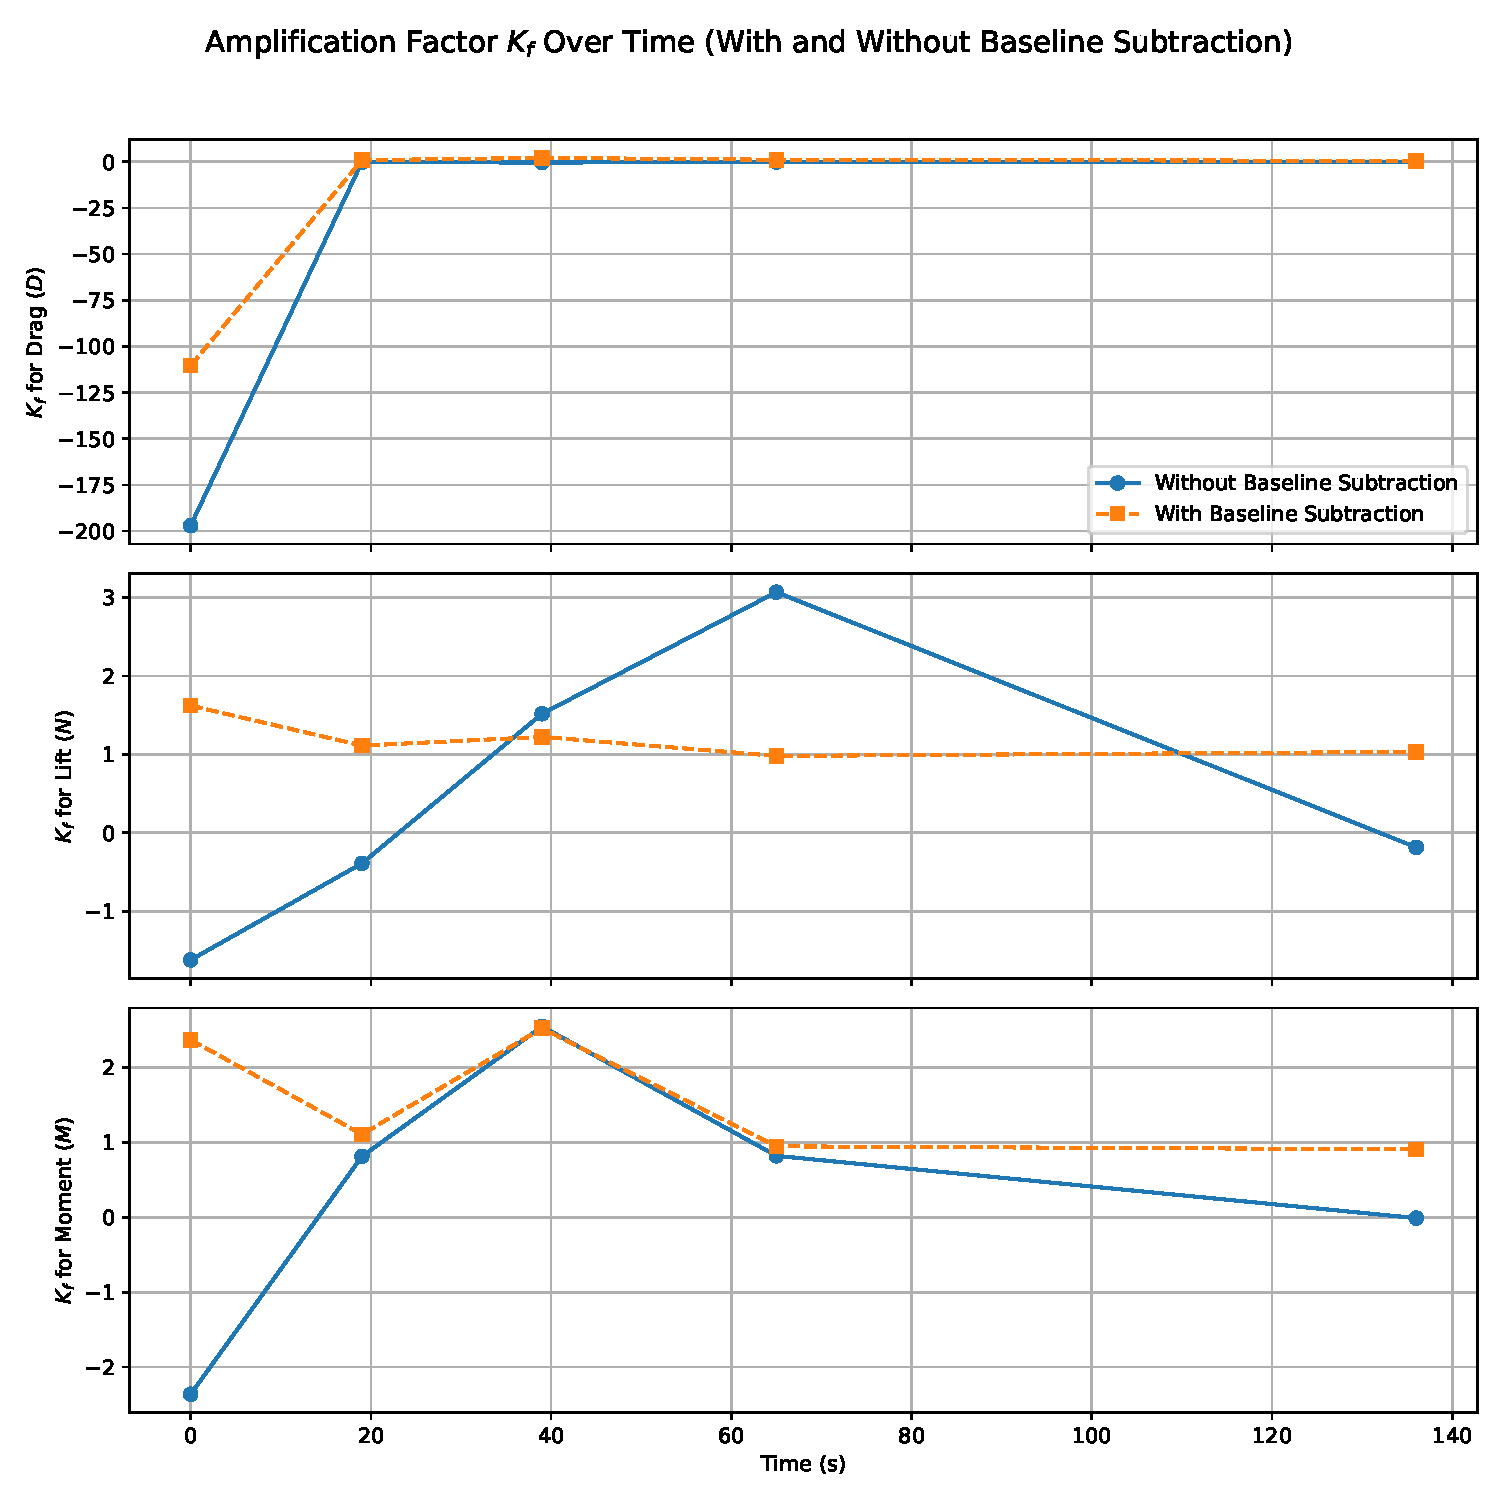
\includegraphics[width=1.0\linewidth]{figs/amplification_factors.pdf}
    %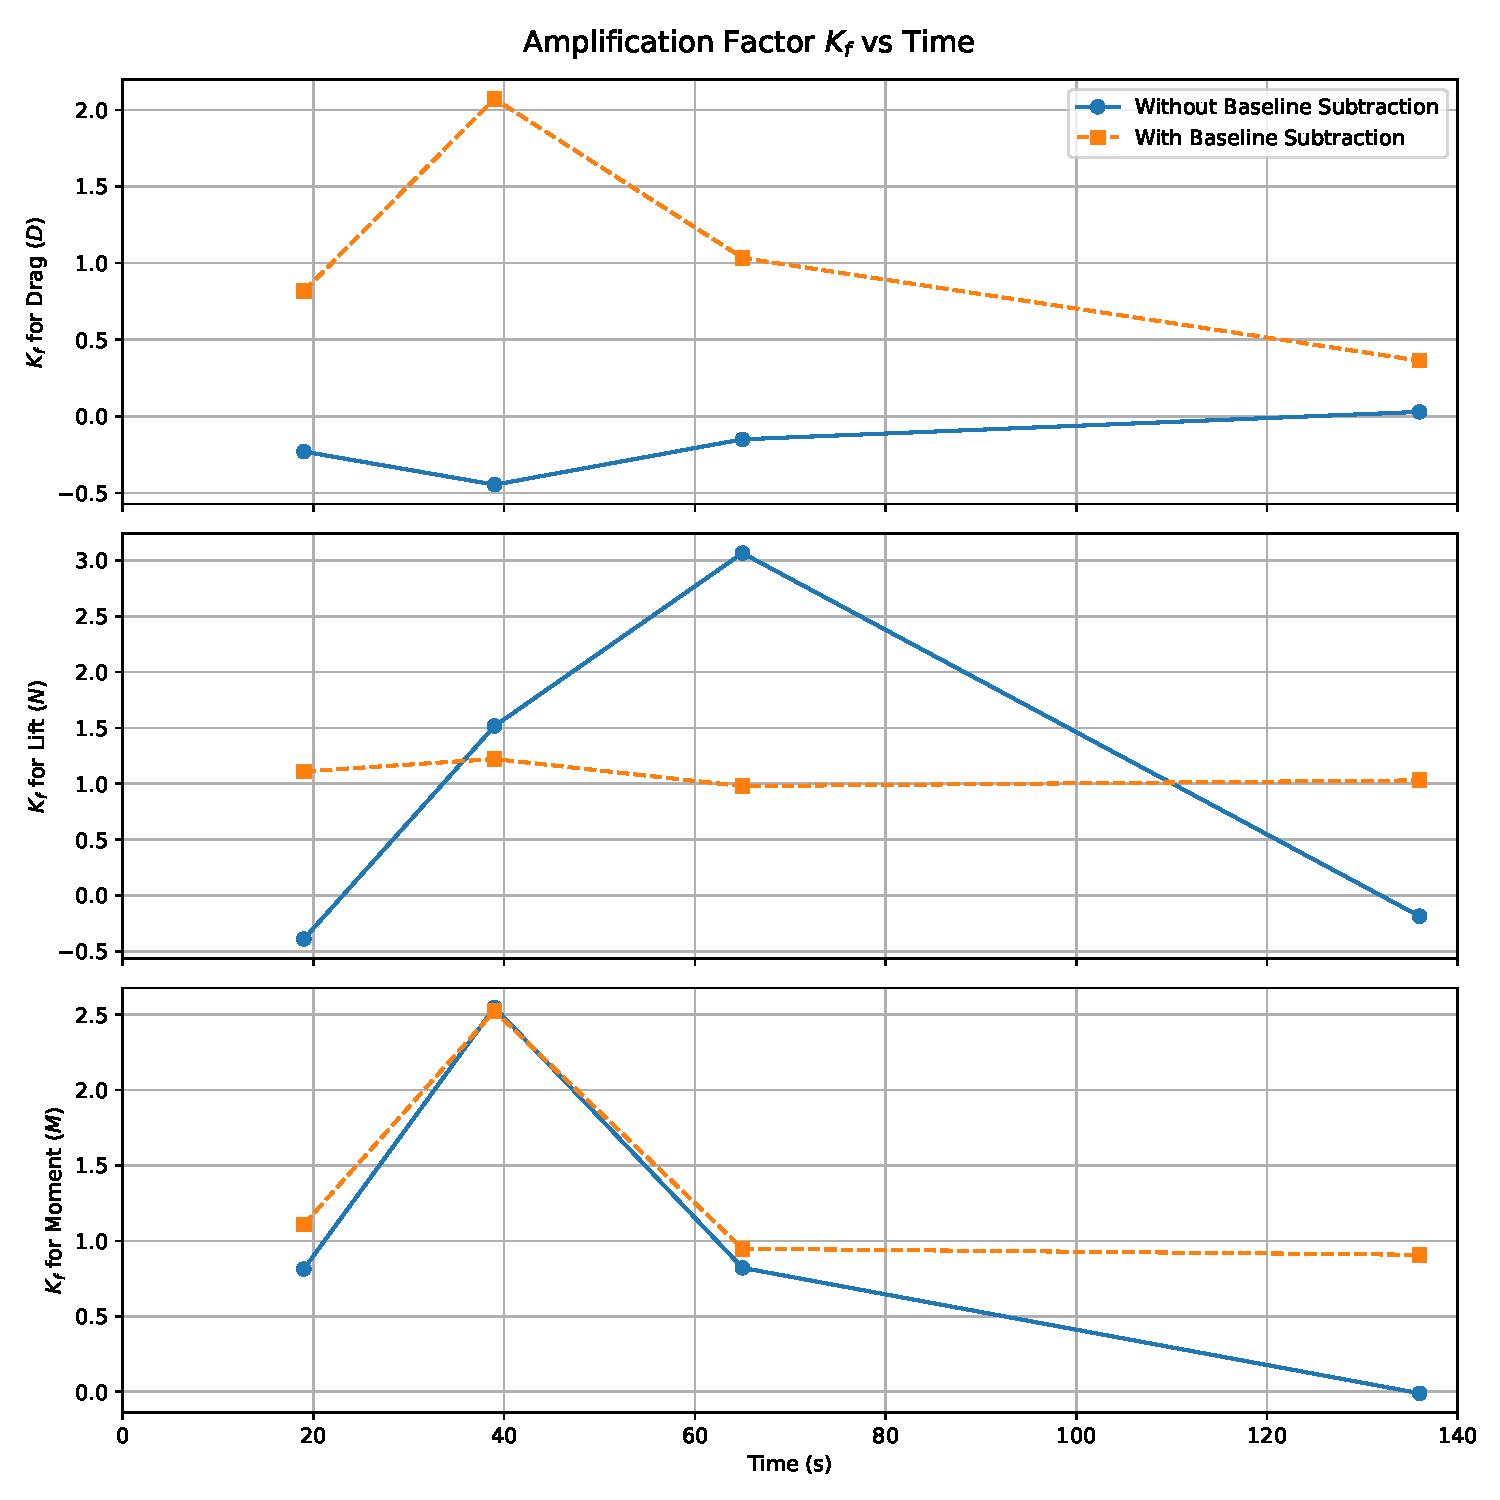
\includegraphics[width=1.0\linewidth]{figs/amplification_factors_no_0.pdf}
    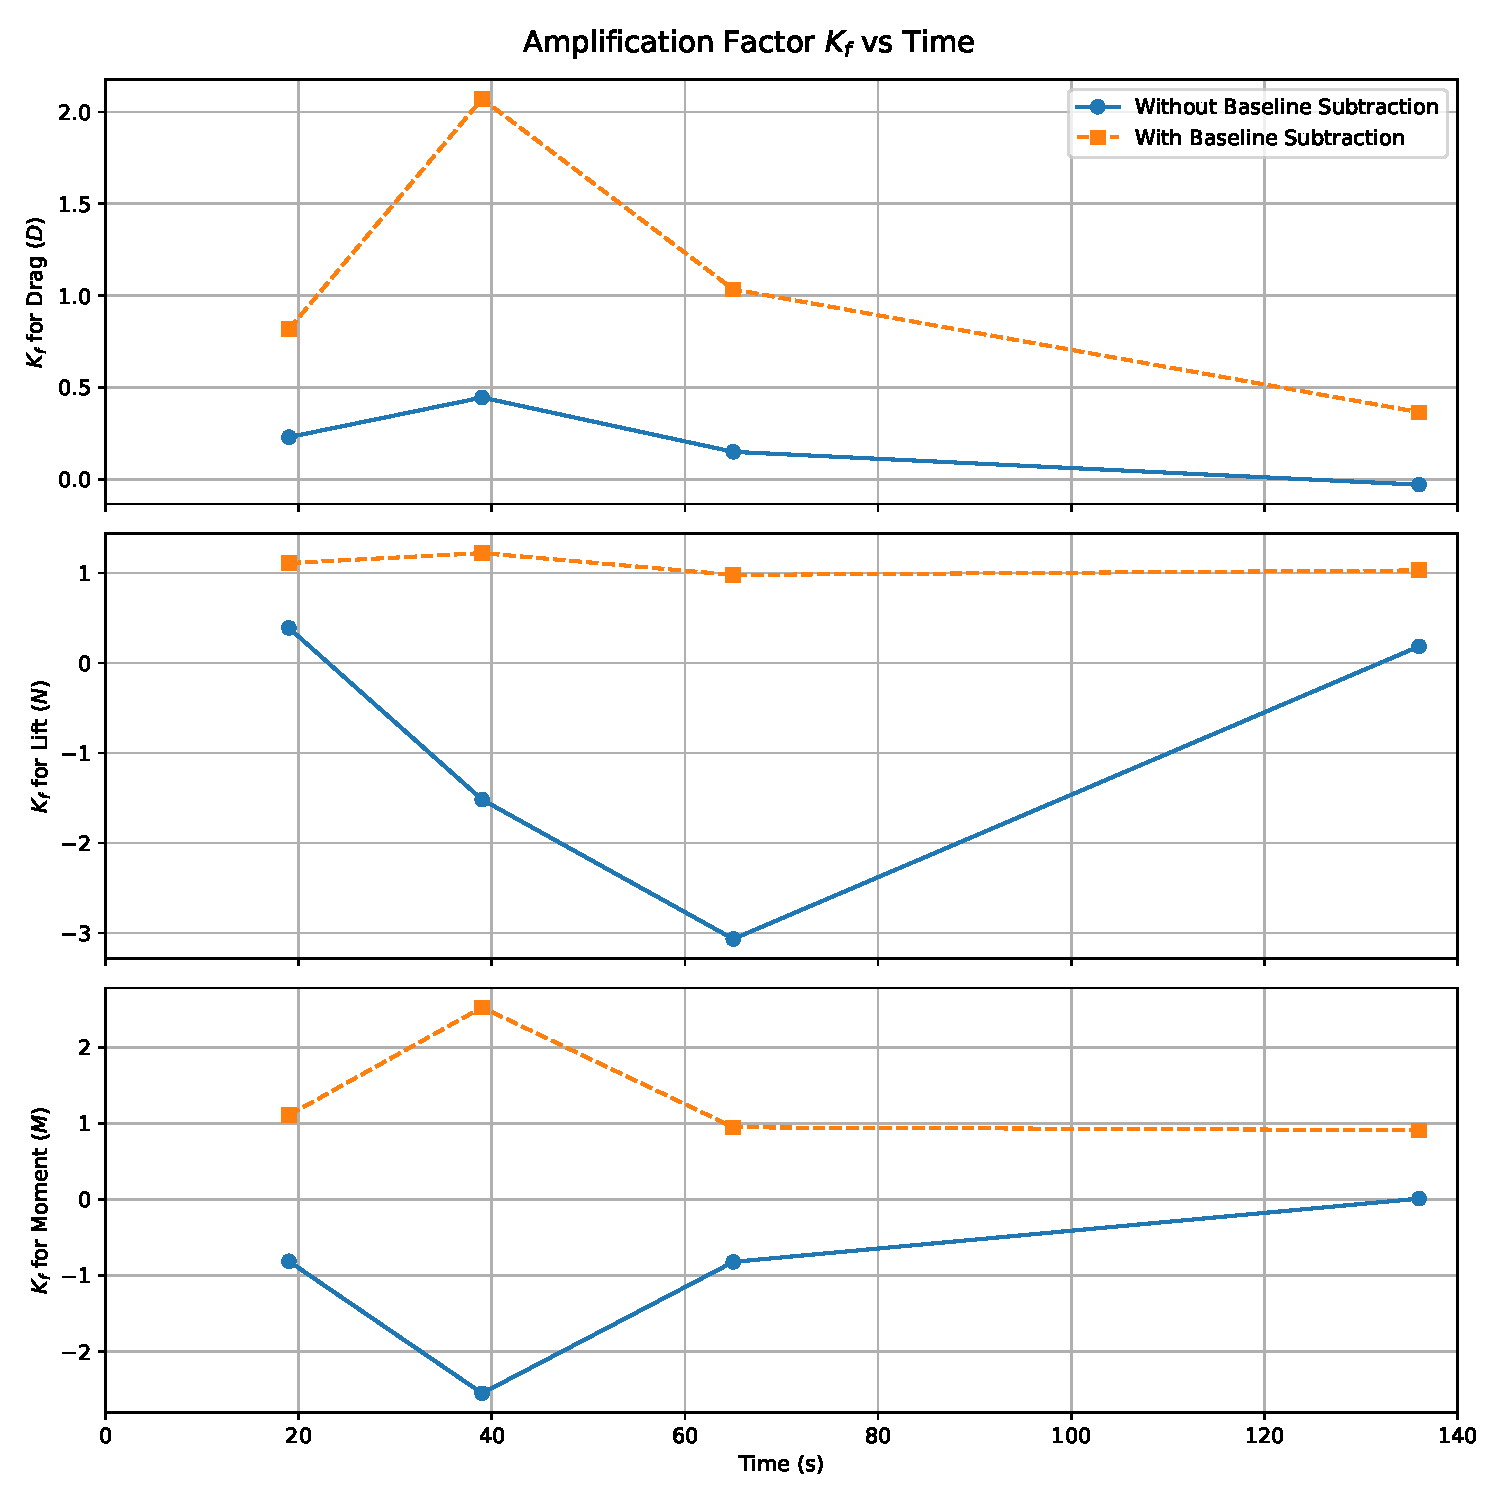
\includegraphics[width=1.0\linewidth]{figs/amplification_factors_vs_Time.pdf}
    \caption{Amplification factor $K_f$ for the drag and normal force and the pitching moment in time.}
    \label{fig:Kf}
\end{figure}

%\begin{table}[H]
%\centering
%\caption{Amplification factors $K_f$ for $C_A$, $C_N$, and $C_M$ with baseline (jetOFFVernierOFF) subtraction.}
%\label{tab:amplification_factors_CA_CN_CM}
%\resizebox{\textwidth}{!}{%
%\begin{tabular}{|c|c|c|c|c|c|c|c|c|c|}
%\hline
%\multirow{2}{*}{Time (s)} & \multicolumn{3}{c|}{$ K_f $ for $ C_A $} & \multicolumn{3}{c|}{$ K_f $ for $ C_N $} & \multicolumn{3}{c|}{$ K_f $ for $ C_M $} \\ \cline{2-10}
%& $ F_j $ & $ F_{\text{baseline}} $ & $ K_f $ & $ F_j $ & $ F_{\text{baseline}} $ & $ K_f $ & $ F_j $ & $ F_{\text{baseline}} $ & $ K_f $ \\ \hline
%0     & 0.612   & 1.700   & -110.75 & 394     & 0.278   & 1.619  & 154    & 0.574   & 2.375  \\ \hline
%19    & 0.692   & 0.498   & 0.814   & 0.734   & 0.477   & 1.093  & 0.29   & 0.503   & 1.094  \\ \hline
%39    & 0.58    & 0.455   & 2.064   & 0.271   & 0.608   & 1.220  & 0.327  & 0.659   & 2.515  \\ \hline
%65    & 0.826   & 0.707   & 1.034   & 0.222   & 0.92    & 0.977  & 0.278  & 0.52    & 0.942  \\ \hline
%136   & 0.270   & 0.292   & 0.364   & -0.528  & -0.433  & 1.042  & -1.53  & -1.52   & 1.000  \\ \hline
%\end{tabular}}
%\end{table}

\begin{table}[H]
\centering
\caption{Test Case Execution at Specific Time Points w.r.t. \textbf{CoM (x=3.3 m)}.}
\label{tab:test_matrix_res_b}
\resizebox{\textwidth}{!}{%
\begin{tabular}{|c|c|c|c|c|c|c|c|c|c|}
\hline
\textbf{Test ID} & \textbf{Sub-Test} & \textbf{Time (s)} & \textbf{CA} & \textbf{CN} & \textbf{CM} & \textbf{Drag (N)} & \textbf{Lift (N)} & \textbf{Moment (Nm)} \\ \hline \hline
%
\multirow{4}{*}{TC000} & jetOFF/VernierOFF & 0 & 1.700 & 0.278 & -0.036 & 5.54 & 0.906 & -0.175 \\ \cline{2-9}
                       & jetOFF/VernierON & 0 & 0.612 & 394 & -712 & 1.99 & 1284 & -3484 \\ \cline{2-9}
                       & jetON/VernierOFF & 0 & 75 & 42.7 & -21.73 & 244 & 139 & -106.3 \\ \cline{2-9}
                       & jetON/VernierON & 0 & 195.5 & 680.2 & -1060 & 636 & 2218 & -5185 \\ \hline \hline
%
\multirow{1}{*}{TC000 fix jet IC} 
%                      & jetOFF/VernierOFF & 0 & - & - & - & - & - & - \\ \cline{2-9}
%                      & jetOFF/VernierOn  & 0 & - & - & - & - & - & - \\ \cline{2-9}
%                      & jetOn/VernierOFF  & 0 & - & - & - & - & - & - \\ \cline{2-9}
                       & jetON/VernierON & 0 & 166.3 & 608.1 & -995.2 & 541 & 1982 & -4867.2 \\ \hline \hline    
%
\multirow{4}{*}{\textbf{TC019}} & jetOFF/VernierOFF & 19 & 0.498 & 0.477 & -0.546 & 1239 & 1186 & -2037 \\ \cline{2-9}
                       & jetOFF/VernierON & 19 & 0.692 & 0.734 & -1.33 & 1721 & 1826 & -4944 \\ \cline{2-9}
                       & jetON/VernierOFF & 19 & 0.82 & 0.92 & -1.03 & 2037 & 2290 & -3850.7 \\ \cline{2-9}
                       & jetON/VernierON & 19 & 0.978 & 1.201 & -1.90 & 2431 & 3001 & -7078 \\ \hline \hline
%                         
\multirow{4}{*}{\textbf{TC039}} & jetOFF/VernierOFF & 39 & 0.455 & 0.608 & -0.68 & 4515 & 6034 & -10117 \\ \cline{2-9}
                       & jetOFF/VernierON & 39 & 0.58 & 0.271 & -0.27 & 5751 & 2692 & -4012 \\ \cline{2-9}
                       & jetON/VernierOFF & 39 & 0.458 & 0.881  & -0.77 & 4542 & 8734 & -11427 \\ \cline{2-9}
                       & jetON/VernierON & 39 & 0.716 & 0.47 & -0.698 & 7103 & 4651 & -10374 \\ \hline \hline
%
\multirow{2}{*}{TC039bis} & jetON/VernierOFF & 39 & 0.52 & 0.715 & \textcolor{green}{-0.84} & 5106 & 6969 & \textcolor{green}{-12264} \\ \cline{2-9}
                       & jetON/VernierON & 39 & 0.6377 & 0.377 & \textcolor{green}{-0.415} & 6208 & 3670 & \textcolor{green}{-6067} \\ \hline \hline
%
\multirow{4}{*}{\textbf{TC065}} 
                       & jetOFF/VernierOFF & 65 & 0.707 & 0.92 & -1.502 & 5720 & 7431 & -18225 \\ \cline{2-9}
                       & jetOFF/VernierON & 65 & 0.876 & 0.222 & -0.205 & 7086 & 1799 & -2485 \\ \cline{2-9}
                       & jetON/VernierOFF & 65 & 0.828 & 0.96 & -1.54 & 6697 & 7764 & -18680 \\ \cline{2-9}
                       & jetON/VernierON & 65 & 0.951 & 0.278 & -0.267 & 7697 & 2248 & -3247 \\ \hline \hline
%
\multirow{1}{*}{TC065 V 50$^\circ$} 
%                       & jetON/VernierOFF  & 65 & - & - & - & - & - & - \\ \cline{2-9}
                        & jetON/VernierON & 65 & 0.935 & 0.343 & -0.375 & 7565 & 2775 & -4550 \\ \hline \hline
%
\multirow{1}{*}{TC065 V1 only} 
%                       & jetON/VernierOFF & 65 & - & - & - & - & - & - \\ \cline{2-9}
                        & jetON/VernierON & 65 & 0.914 & 0.642 & -0.927 & 7392 & 5194 & -11249 \\ \hline \hline                        
%                        
\multirow{4}{*}{\textbf{TC136}} & jetOFF/VernierOFF & 136 & 0.292 & -0.433 & -0.565 & 581 & -861 & -1685 \\ \cline{2-9}
                       & jetOFF/VernierON & 136 & 0.270 & -0.528 & -0.37 & 537 & -1051 & -1107 \\ \cline{2-9}
                       & jetON/VernierOFF & 136 & 0.28 & -0.435 & -0.56 & 557 & -866  & -1667 \\ \cline{2-9}
                       & jetON/VernierON & 136 & 0.272 & -0.534 & -0.358 & 541 & -1062 & -1067 \\ \hline \hline
%
\end{tabular}}
\end{table}

\begin{table}[H]
\centering
\caption{Amplification Factors $ K_f $ for Drag ($ D $), Lift ($ N $), and Moment ($ M $) with Baseline Subtraction (CoM)}
\label{tab:amplification_factors_DNM_CoM}
\resizebox{\textwidth}{!}{%
\begin{tabular}{|c|c|c|c|c|c|c|c|c|c|}
\hline
\multirow{2}{*}{Time (s)} & \multicolumn{3}{c|}{$ K_f $ for Drag $ D $} & \multicolumn{3}{c|}{$ K_f $ for Lift $ N $} & \multicolumn{3}{c|}{$ K_f $ for Moment $ M $} \\ \cline{2-10}
& $ F_j $ & $ F_{\text{baseline}} $ & $ K_f $ & $ F_j $ & $ F_{\text{baseline}} $ & $ K_f $ & $ F_j $ & $ F_{\text{baseline}} $ & $ K_f $ \\ \hline
0     & 1.99   & 5.54   & -110.4 & 1284   & 0.906  & 1.620  & -3484  & -0.175 & 1.458  \\ \hline
19    & 1721   & 1239   & 0.817  & 1826   & 1186   & 1.111  & -4944  & -2037  & 1.110  \\ \hline
39    & 5751   & 4515   & 2.072  & 2692   & 6034   & 1.222  & -4012  & -10117 & 0.173  \\ \hline
65    & 7086   & 5720   & 0.732  & 1799   & 7431   & 0.979  & -2485  & -18225 & 0.981  \\ \hline
136   & 537    & 581    & 0.364  & -1051  & -861   & 1.032  & -1107  & -1685  & 1.038  \\ \hline
\end{tabular}}
\end{table}

\begin{table}[H]
\centering
\caption{Amplification Factors $ K_f $ for Drag ($ D $), Lift ($ N $), and Moment ($ M $) without Baseline Subtraction (CoM)}
\label{tab:amplification_factors_DNM_CoM_no_base}
\resizebox{\textwidth}{!}{%
\begin{tabular}{|c|c|c|c|c|c|c|c|c|c|}
\hline
\multirow{2}{*}{Time (s)} & \multicolumn{3}{c|}{$ K_f $ for Drag $ D $} & \multicolumn{3}{c|}{$ K_f $ for Lift $ N $} & \multicolumn{3}{c|}{$ K_f $ for Moment $ M $} \\ \cline{2-10}
& $ F_j $ & $ F_{\text{no-jet}} $ & $ K_f $ & $ F_j $ & $ F_{\text{no-jet}} $ & $ K_f $ & $ F_j $ & $ F_{\text{no-jet}} $ & $ K_f $ \\ \hline
0     & 1.99   & 244   & 197.0  & 1284   & 139   & 1.620  & -3484  & -106.3 & 1.458  \\ \hline
19    & 1721   & 2037  & 0.229  & 1826   & 2290  & 0.390  & -4944  & -3850.7 & 0.653  \\ \hline
39    & 5751   & 4542  & 0.445  & 2692   & 8734  & -1.517 & -4012  & -11427 & -0.262 \\ \hline
65    & 7086   & 6697  & 0.141  & 1799   & 7764  & -3.066 & -2485  & -18680 & -6.21  \\ \hline
136   & 537    & 557   & -0.030 & -1051  & -866  & 0.186  & -1107  & -1667  & -0.542 \\ \hline
\end{tabular}}
\end{table}

\begin{table}[H]
\centering
\caption{Amplification Factors $ A_D $, $ A_N $, and $ A_M $ Based on Jet-Only and Jet+JI Cases (CoM Reference)}
\label{tab:amplification_factors_A}
\resizebox{\textwidth}{!}{%
\begin{tabular}{|c|c|c|c|c|c|c|c|}
\hline
\multirow{2}{*}{Time (s)} & \multicolumn{2}{c|}{$ A_D $} & \multicolumn{2}{c|}{$ A_N $} & \multicolumn{2}{c|}{$ A_M $} \\ \cline{2-7}
& $ F_j $ & $ A_D $ & $ F_j $ & $ A_N $ & $ M_j $ & $ A_M $ \\ \hline
0     & 244   & 2.607  & 139   & 15.957  & -106.3  & 48.777  \\ \hline
19    & 2037  & 1.193  & 2290  & 1.310   & -3850.7 & 1.838   \\ \hline
39    & 4542  & 1.564  & 8734  & 0.533   & -11427  & 0.908   \\ \hline
65    & 6697  & 1.149  & 7764  & 0.290   & -18680  & 0.174   \\ \hline
136   & 557   & 0.971  & -866  & 1.226   & -1667   & 0.640   \\ \hline
\end{tabular}}
\end{table}

%\begin{figure}[H]
%    \centering
%    %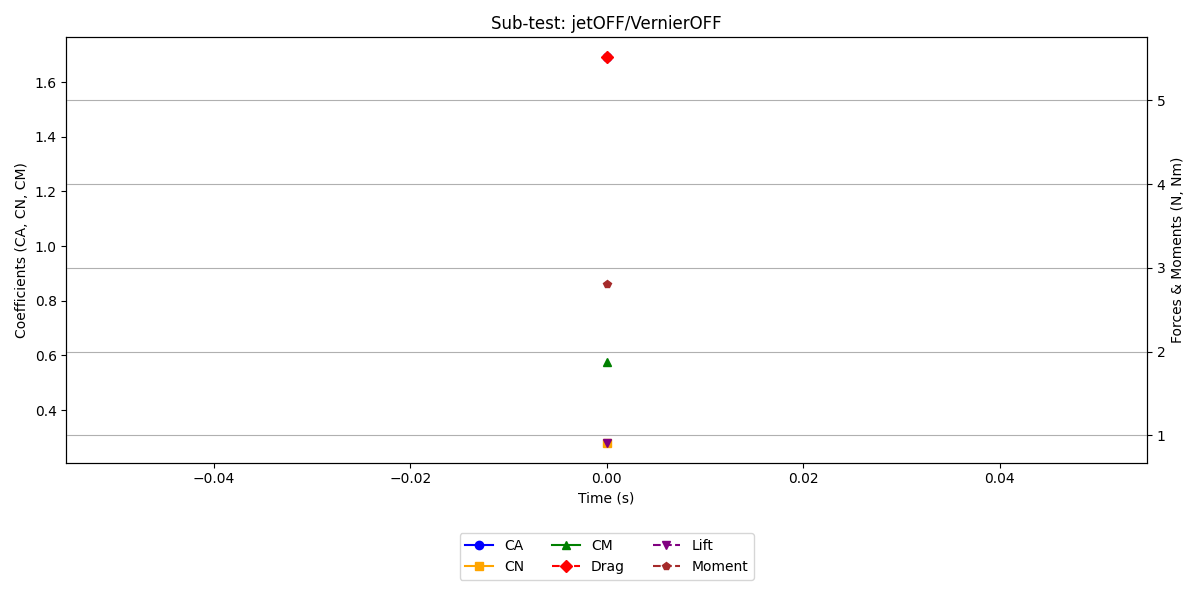
\includegraphics[width=0.495\linewidth]{figs/Figure_subtestOFFOFF.png}
%    %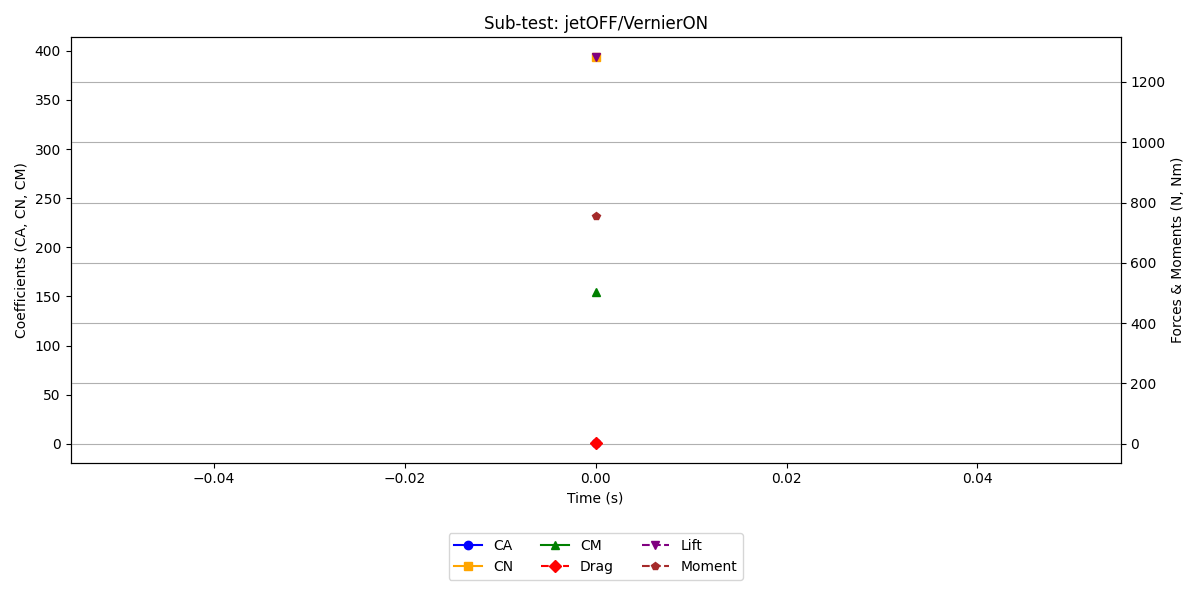
\includegraphics[width=0.495\linewidth]{figs/Figure_subtestOFFON.png}\\
%    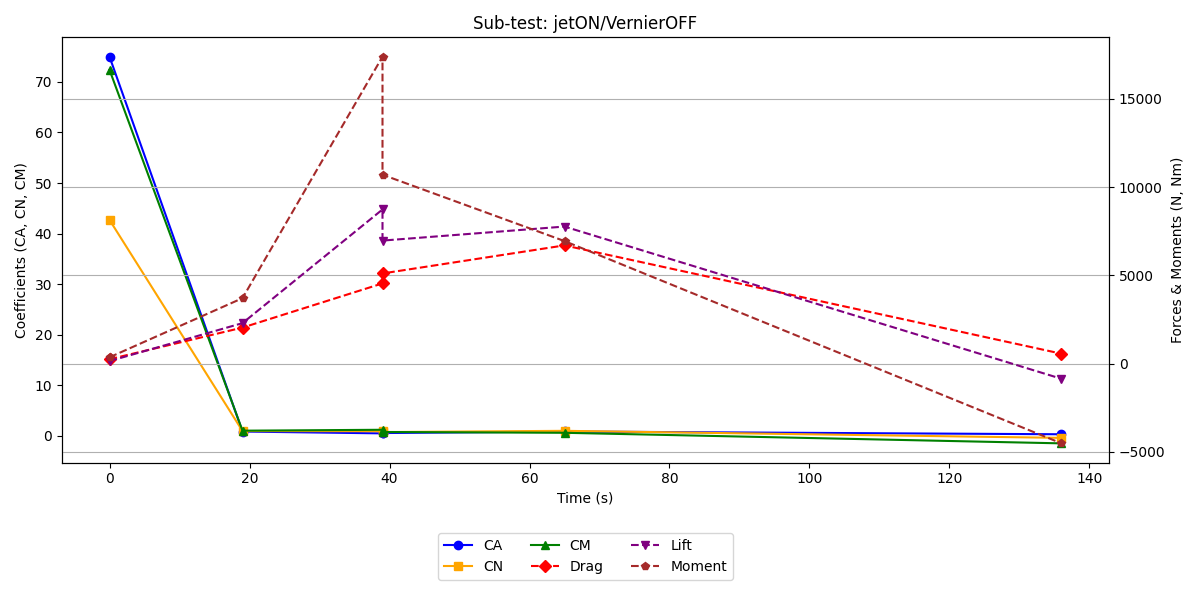
\includegraphics[width=\linewidth]{figs/Figure_subtestONOFF.png}\\
%    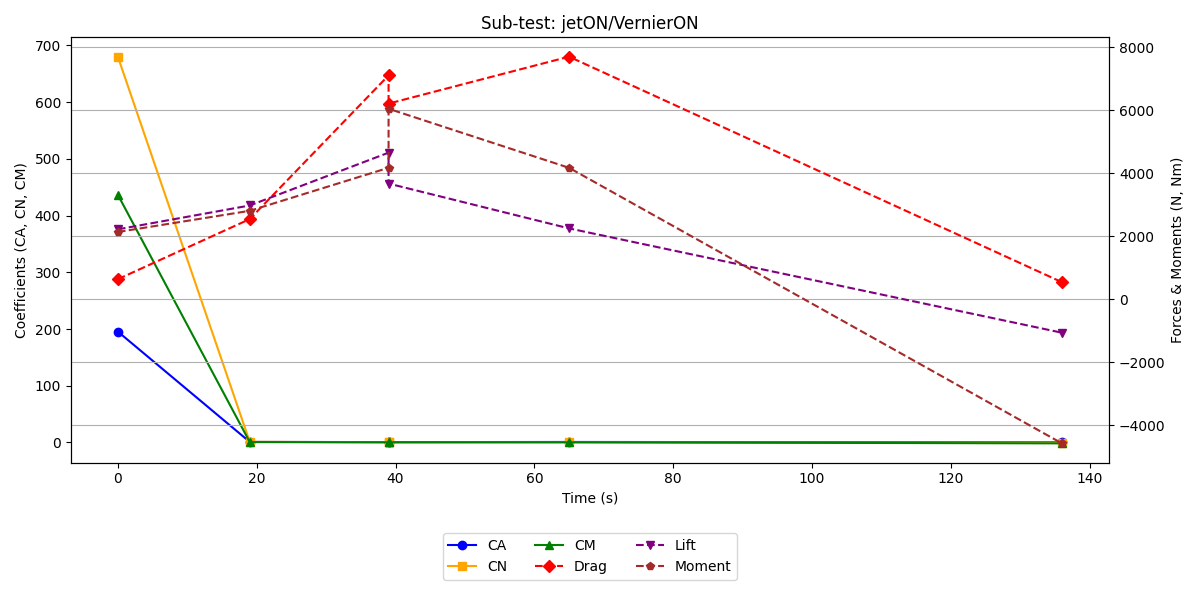
\includegraphics[width=\linewidth]{figs/Figure_subtestONON.png}
%    \caption{Variation of aerodynamic coefficients (CA, CN, CM) and corresponding forces and moment (Drag, Lift, Moment) over time for test cases with thrusters activated (jetON) and vernier nozzles deactivated (VernierOFF). Time points include 0 s (baseline), 19 s, 39 s, 65 s, and 136 s.}
%    \label{fig:jetonoff}
%\end{figure}
%
%\begin{figure}[H]
%    \centering
%    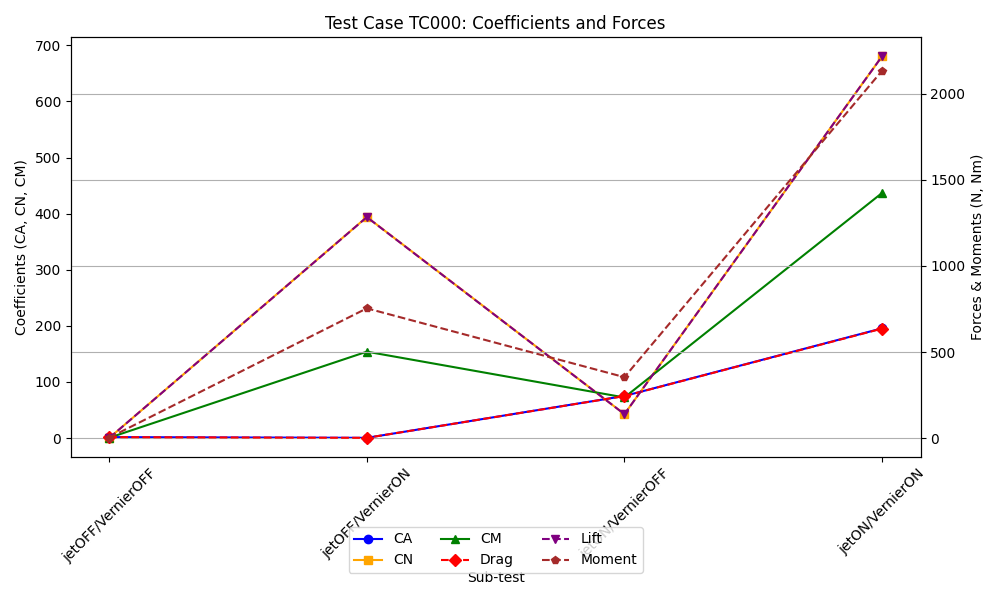
\includegraphics[width=0.495\linewidth]{figs/Figure_TC000.png}
%    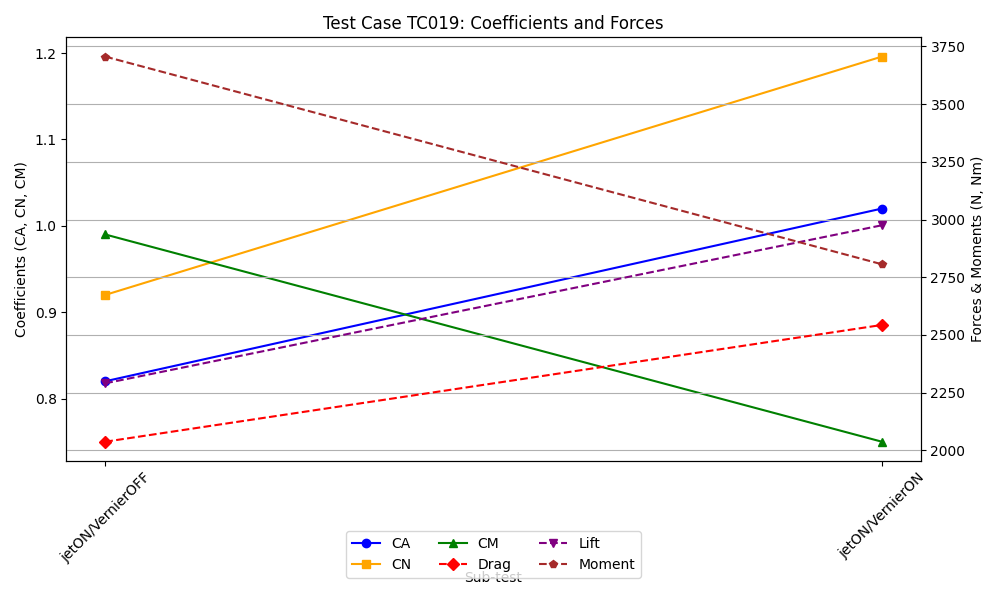
\includegraphics[width=0.495\linewidth]{figs/Figure_TC019.png}\\
%    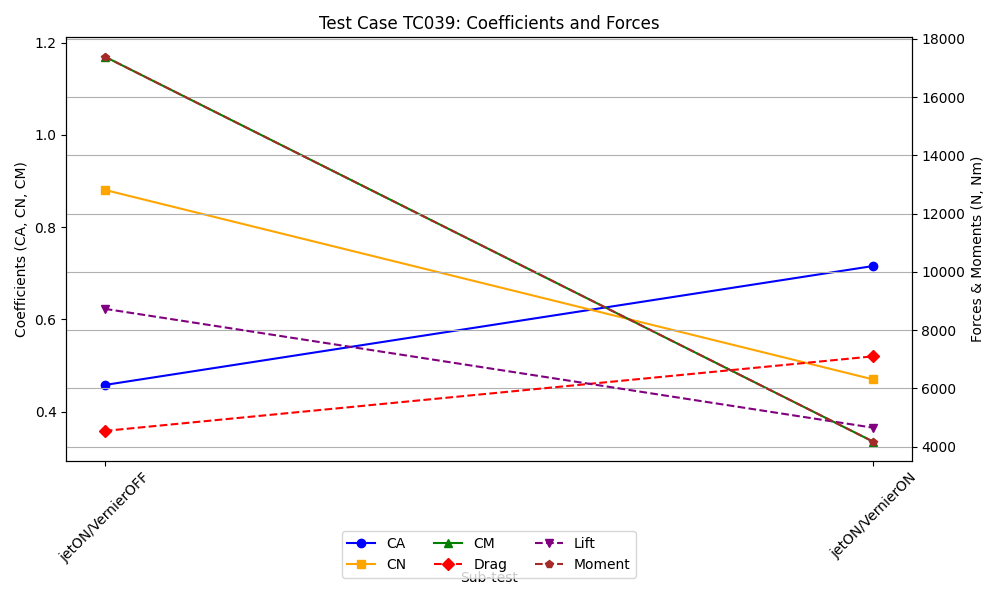
\includegraphics[width=0.495\linewidth]{figs/Figure_TC039.png}
%    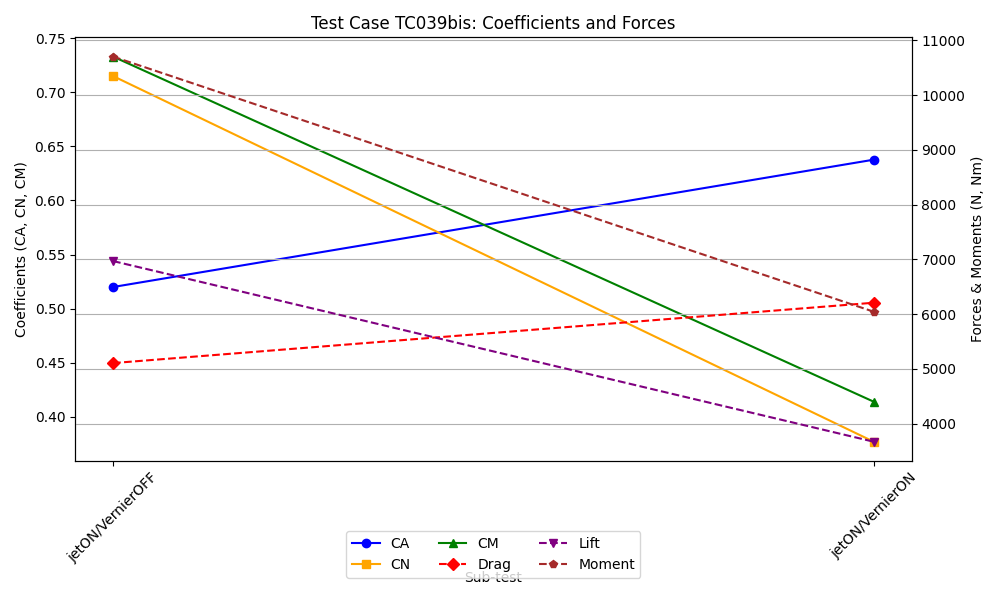
\includegraphics[width=0.495\linewidth]{figs/Figure_TC039bis.png}\\
%    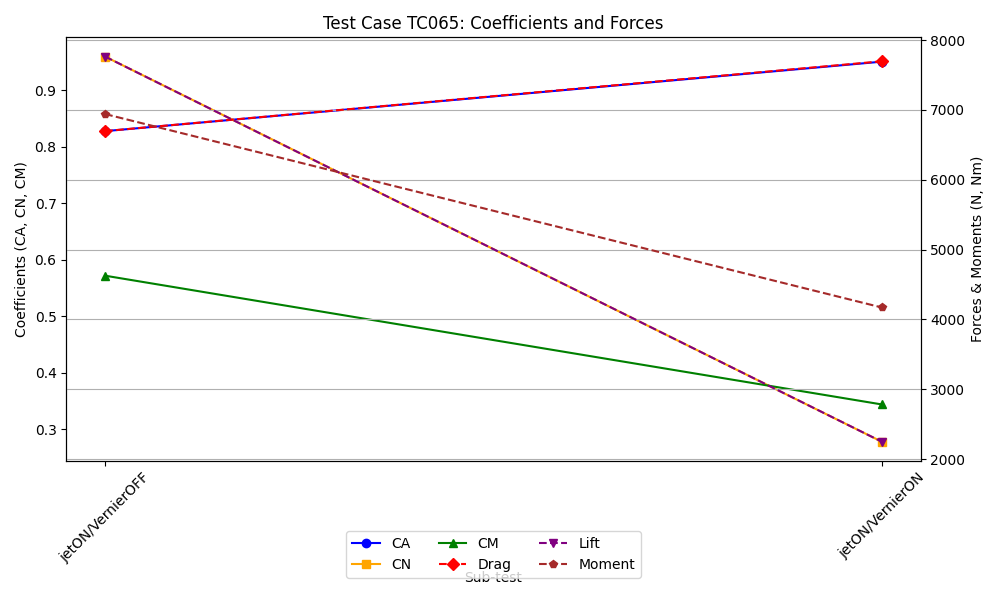
\includegraphics[width=0.495\linewidth]{figs/Figure_TC065.png}
%    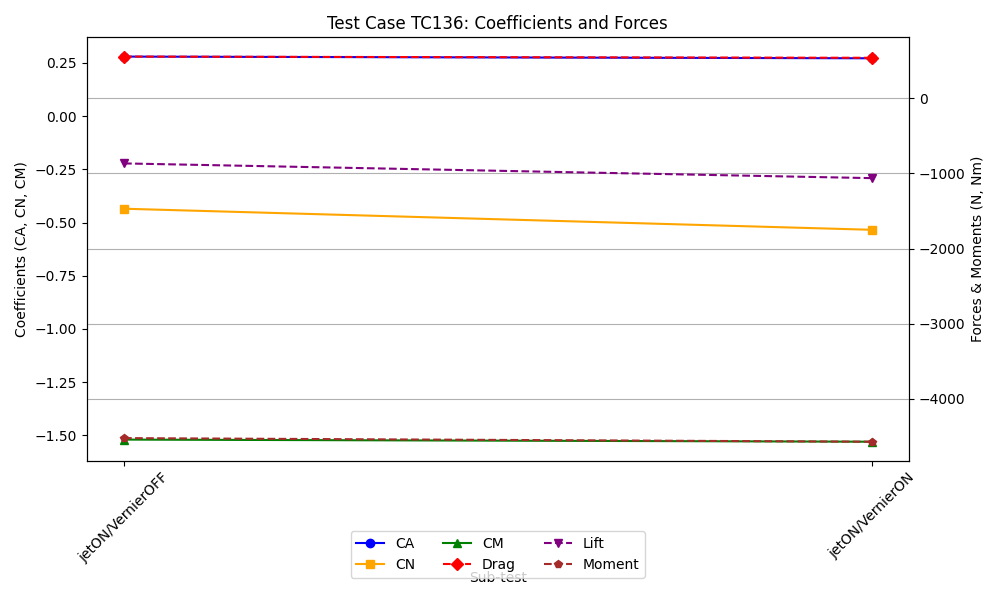
\includegraphics[width=0.495\linewidth]{figs/Figure_TC136.png}\\
%    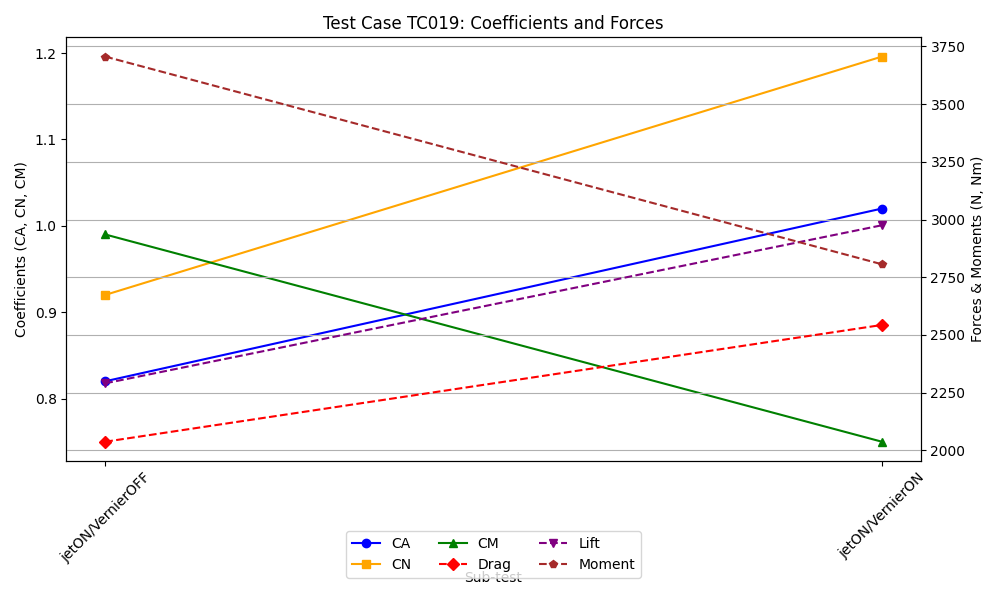
\includegraphics[width=0.495\linewidth]{figs/Figure_TC019.png}
%    \caption{Variation of aerodynamic coefficients (CA, CN, CM) and corresponding forces and moment (Drag, Lift, Moment) across different thruster configurations at different times. Sub-tests include combinations of main jet (jetON/OFF) and vernier nozzle (VernierON/OFF) activation states.}
%    \label{fig:subtestcase}
%\end{figure}

\begin{table}[H]
\centering
\caption{Combined Test Case Execution with $\Delta$ Pitching Moment at CoM.}
\label{tab:combined_with_delta}
\resizebox{\textwidth}{!}{%
\begin{tabular}{|c|c|c|c|c|c|c|c|}
\hline
\textbf{Test ID} & \textbf{Sub-Test} & \textbf{Time (s)} & \textbf{CM (Base)} & \textbf{Moment (Base)} & \textbf{CM (CoM)} & \textbf{Moment (CoM)} & \textbf{$\Delta$ Pitching Moment (\textit{X$_{COM}$}) with Verniers (Nm)} \\ \hline \hline

TC000 & jetOFF/VernierOFF & 0 & 0.574 & 2.807 & -0.037 & -0.181 & — \\ \hline
TC000 & jetOFF/VernierON  & 0 & 154   & 754   & -712    & -3484  & $-3484 - (-0.181) =$ \textbf{-3483.8} \\ \hline
TC000 & jetON/VernierOFF  & 0 & 72.4  & 354   & -21.7   & -106.3 & — \\ \hline
TC000 & jetON/VernierON   & 0 & 436.7 & 2134  & -1060   & -5185  & $-5185 - (-106.3) =$ \textbf{-5078.7} \\ \hline \hline

TC019 & jetON/VernierOFF  & 19 & 0.99   & 3706   & -1.03   & -3850.7 & - \\ \cline{1-8}
TC019 & jetON/VernierON   & 19 & 0.75   & 2806   & -1.88   & -7011.4 & $-7011.4 - (-3850.7) =$ \textbf{-3160.7} \\ \hline \hline

TC039 & jetON/VernierOFF  & 39 & 1.17   & 17394  & -0.77   & -11427 & - \\ \cline{1-8}
TC039 & jetON/VernierON   & 39 & 0.335  & 4171   & -0.698  & -10374 & $-10374 - (-11427) =$ \textbf{1053} \\ \hline \hline

TC039bis & jetON/VernierOFF  & 39 & 0.733 & 10703 & -0.84  & -12264 & - \\ \cline{1-8}
TC039bis & jetON/VernierON   & 39 & 0.414 & 6044  & -0.415 & -6067  & $-6067 - (-12264) =$ \textbf{\textcolor{green}{6197}} \\ \hline \hline

TC065 & jetON/VernierOFF  & 65 & 0.572  & 6941   & -1.54   & -18680 & - \\ \cline{1-8}
TC065 & jetON/VernierON   & 65 & 0.344  & 4170.6 & -0.267  & -3246  & $-3246 - (-18680) =$ \textbf{15434} \\ \hline \hline

TC136 & jetON/VernierOFF  & 136 & -1.52  & -4525  & -0.56   & -1667  & - \\ \cline{1-8}
TC136 & jetON/VernierON   & 136 & -1.53  & -4573  & -0.358  & -1067  & $-1067 - (-1667) =$ \textbf{600} \\ \hline

\end{tabular}}
\end{table}

\begin{figure}[H]
    \centering
    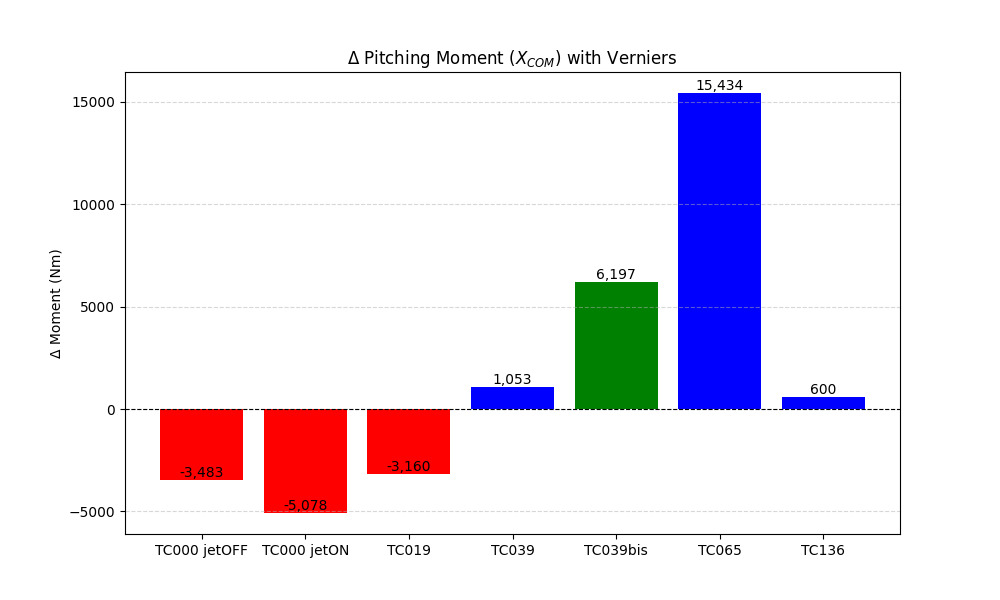
\includegraphics[width=\linewidth]{figs/DeltaPmoment.png}
    \caption{{$\Delta$ Pitching Moment (Nm) w.r.t. \textit{X$_{COM}$} due to the action of the Verniers.} The green bar was calculated from the "new" trajectory point flight conditions at t = 39 s provided by Luca.}
    \label{fig:DPmoment}
\end{figure}

%\begin{table}[H]
%\centering
%\caption{Test Case Execution at Specific Time Points (hand-calc. by Kyle)}
%\label{tab:test_matrix}
%\resizebox{\textwidth}{!}{%
%\begin{tabular}{|c|c|c|c|c|c|c|c|c|}
%\hline
%\textbf{Test ID} & \textbf{Sub-Test} & \textbf{Time (s)} & \textbf{CA} & \textbf{CN} & \textbf{CM} & \textbf{Pitching Moment (Base) (Nm)} & \textbf{Pitching Moment ($X_{COM}$) (Nm)} & \textbf{$\Delta $Pitching Moment ($X_{COM}$) with Verniers(Nm)} \\ \hline \hline
%
%\multirow{4}{*}{TC000} & jetOFF, VernierOFF & 0 & 1.693 & 0.278 & 0.574 & 2.8 & -0.2 &  N/A\\ \cline{2-9}
%                       & jetOFF, VernierON  & 0 & 0.421 & 394   & 154   & 754 & -3485& \\ \cline{2-9}
%                       & jetON, VernierOFF  & 0 & 75    & 42.7  & 72.4  & 354 & -105& \\\cline{2-9}
%                       & jetON, VernierON   & 0 & 195.5 & 680.2 & 436.7 & 2134 & -5182&\\ \hline \hline
%%
%\multirow{2}{*}{TC019} & jetON, VernierOFF  & 19 & 0.82 & 0.92 & 0.99 & 4021 & -4189&\\ \cline{2-9}
%                       & jetON, VernierON   & 19 & 1.02 & 1.196 & 0.75 & 3047 & -7621 &\\ \hline \hline
%%                         
%\multirow{2}{*}{TC039} & jetON, VernierOFF  & 39 & 0.458 & 0.881  & 1.17 & 17394 & -11423& \\ \cline{2-9}
%       & jetON, VernierON   & 39 & \textit{0.716} & \textit{0.447} & \textit{0.446} & \textit{6641} & -7991&\\ \hline \hline
%%
%\multirow{2}{*}{TC065} & jetON, VernierOFF  & 65 & 0.828 & 0.96 & 0.572 & 6941.5 & -18691& \\ \cline{2-9}
%                       & jetON, VernierON   & 65 & 0.951 & 0.278 & 0.344 & 4170.6 & -3247 &            \\ \hline \hline
%%                        
%\multirow{2}{*}{TC136} & jetON, VernierOFF  & 136 & 0.28 & 0.435 & 1.52 & 4530 &1679 &\\ \cline{2-9}
%                       & jetON, VernierON   & 136 & 0.27 & 0.53  & 1.53 & 4573 & 1085 &\\ \hline \hline
%%
%\end{tabular}%
%}
%\end{table}

%%%%%%%%%%%%%%%%%%%%%%%%%%%%%%%%%%%%%%%%%%%%%%%%%%%%%%
\subsection{Amplification}\label{sec:amplification}
%%%%%%%%%%%%%%%%%%%%%%%%%%%%%%%%%%%%%%%%%%%%%%%%%%%%%%

The amplification of the vernier force shall be evaluated using several points. First start with the jetOFF comparison at $t=0~s$. 

\begin{align}
    f_{v_{pressure}} &= a_v \cdot \Delta P
\end{align}

Consider atmospheric pressure $P_{\inf}=101325Pa$. Also, consider that the vernier plume pressure is $P_{plume}\approx 25000Pa$.

\begin{align}
    \Delta P = P_{\inf}-P_{plume}= 75000Pa
\end{align}

Finally, consider the area of the vernier face (assumed flat) $A_v = \frac{\pi\cdot0.05\cdot0.05}{4} = 0.00196\;m^2$, as diameter of the vernier outlet is $\approx 50~mm$. Therefore, the pressure force on the vernier is:

\begin{align}
    f_{v_{pressure}} &= a_v \cdot \Delta P\\
     &= 0.00196 \cdot 75000\\
     &=147.2N
\end{align}

Based on the JetOFF/VernierOFF case, we see that the vernier force is:

\begin{table}[H]
\centering
\caption{Amplification of Vernier Force Based on Pressure Difference}
\resizebox{\textwidth}{!}{%
\begin{tabular}{|c|c|c|c|c|c|c}
\hline
\textbf{Test ID} & \textbf{Sub-Test} & \textbf{Time (s)} & \textbf{calculated $f_{v_{pressure}}$} & \textbf{observed $f_{v_{pressure}}$} & \textbf{Amplification} \\ \hline \hline
\multirow{4}{*}{TC000} & jetOFF, VernierOFF & 0 & $=0.00258\cdot(101325-101325) = 0~N$ & $2.8/3.3(x_{COM})/2(\times \;verniers) = 0.42N$ & N/A \\ \cline{2-6}
                       & jetOFF, VernierON  & 0 &  $=0.00258\cdot(101325-32443) = 177.7~N$ & 754/3.3/2 = $114~N$& \\ \cline{2-6}
                       & jetON, VernierOFF  & 0 & $0~N$ & 354/3.3/2 = $54~N$ & N/A \\ \cline{2-6}
                       & jetON, VernierON   & 0 & $159~N$ & 2134/3.3/2 = $323~N$ & \\ \hline \hline
%
\multirow{2}{*}{TC019} & jetON, VernierOFF  & 19 & $0~N$ & & N/A \\ \cline{2-6}
                       & jetON, VernierON   & 19 & 172 N & 428.2 N & \\ \hline \hline
%                         
\multirow{2}{*}{TC039} & jetON, VernierOFF  & 39 & $0~N$ & & N/A \\ \cline{2-6}
              & jetON, VernierON   & 39 & 91 N & 753.8 N &  \\ \hline \hline
%
\multirow{2}{*}{TC065} & jetON, VernierOFF  & 65 & $0~N$ & & N/A \\ \cline{2-6}
                       & jetON, VernierON   & 65 & -4.6 N & 632 N & \\ \hline \hline
%                        
\multirow{2}{*}{TC136} & jetON, VernierOFF  & 136 & $0~N$ & & N/A \\ \cline{2-6}
                       & jetON, VernierON   & 136 & -62 N & -692.9 N & \\ \hline \hline
%
\end{tabular}}
\end{table}

%\begin{table}[H]
%\centering
%\caption{Amplification of Vernier Force Based on Pressure Difference}
%\label{tab:amplification_venier_force}
%\resizebox{\textwidth}{!}{%
%\begin{tabular}{|c|c|c|c|c|c|}
%\hline
%\textbf{Test ID} & \textbf{Sub-Test} & \textbf{Time (s)} & \textbf{Calculated $ f_{v_{\text{pressure}}} $} & \textbf{Observed $ f_{v_{\text{pressure}}} $} & \textbf{Amplification $ K $} \\ \hline \hline
%\multirow{4}{*}{TC000} & jetOFF/VernierOFF & 0 & $ 0.00258 \cdot (101325 - 101325) = 0 $ N & $ 2.8 / 3.3 / 2 = 0.42 $ N & N/A \\ \cline{2-6}
%                       & jetOFF/VernierON & 0 & $ 0.00258 \cdot (101325 - 32443) = 177.7 $ N & $ 754 / 3.3 / 2 = 114 $ N & — \\ \cline{2-6}
%                       & jetON/VernierOFF & 0 & $ 0.00258 \cdot (101325 - 101325) = 0 $ N & $ 354 / 3.3 / 2 = 54 $ N & — \\ \cline{2-6}
%                       & jetON/VernierON & 0 & $ 0.00258 \cdot (101325 - 101325) = 0 $ N & $ 2134 / 3.3 / 2 = 323 $ N & $ \frac{323 - 114}{114 - 0} = 1.83 $ \\ \hline \hline
%
%\multirow{2}{*}{TC019} & jetON/VernierOFF & 19 & $ 0.00258 \cdot (101325 - 101325) = 0 $ N & $ 2290 / 3.3 / 2 = 347 $ N & — \\ \cline{2-6}
%                       & jetON/VernierON & 19 & $ 0.00258 \cdot (101325 - 70135) = 80.3 $ N & $ 3001 / 3.3 / 2 = 455 $ N & $ \frac{455 - 347}{347 - 0.42} = 0.31 $ \\ \hline \hline
%
%\multirow{2}{*}{TC039} & jetON/VernierOFF & 39 & $ 0.00258 \cdot (101325 - 101325) = 0 $ N & $ 8734 / 3.3 / 2 = 1323 $ N & — \\ \cline{2-6}
%                       & jetON/VernierON & 39 & $ 0.00258 \cdot (101325 - 90000) = 29.2 $ N & $ 4651 / 3.3 / 2 = 705 $ N & $ \frac{705 - 1323}{1323 - 114} = -0.51 $ \\ \hline \hline
%
%\multirow{2}{*}{TC065} & jetON/VernierOFF & 65 & $ 0.00258 \cdot (101325 - 101325) = 0 $ N & $ 7764 / 3.3 / 2 = 1176 $ N & — \\ \cline{2-6}
%                       & jetON/VernierON & 65 & $ 0.00258 \cdot (101325 - 99000) = 6.0 $ N & $ 2248 / 3.3 / 2 = 341 $ N & $ \frac{341 - 1176}{1176 - 54} = -0.74 $ \\ \hline \hline
%
%\multirow{2}{*}{TC136} & jetON/VernierOFF & 136 & $ 0.00258 \cdot (101325 - 101325) = 0 $ N & $ -866 / 3.3 / 2 = -131 $ N & — \\ \cline{2-6}
%                       & jetON/VernierON & 136 & $ 0.00258 \cdot (101325 - 100000) = 3.4 $ N & $ -1062 / 3.3 / 2 = -161 $ N & $ \frac{-161 - (-131)}{-131 - 0.42} = 0.23 $ \\ \hline \hline
%\end{tabular}}
%\end{table}

\begin{figure}[H]
    \centering
    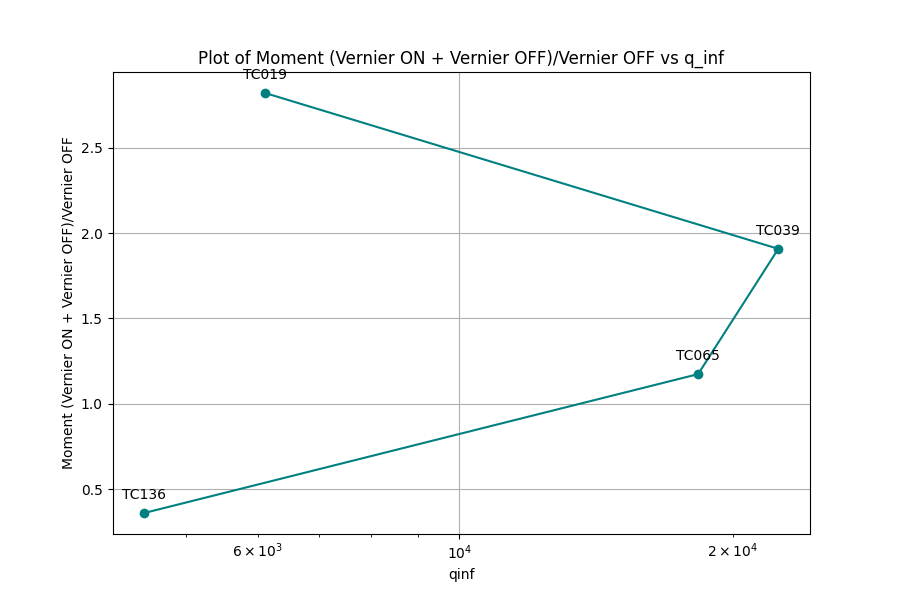
\includegraphics[width=\linewidth]{figs/M_vs_qinf.png}
    \caption{Moment (total/jet ON only) taken from Table~\ref{tab:test_matrix_res_b} with $q_{inf}$.}
    \label{fig:M_vs_qinf}
\end{figure}

%\begin{table}[H]
%\centering
%\caption{Test}
%\resizebox{\textwidth}{!}{%
%\begin{tabular}{|c|c|c|c|c|c|}
%\hline
%\textbf{Test ID} & \textbf{Sub-Test} & \textbf{Time (s)} & \textbf{calculated $f_{v_{pressure}}$} & \textbf{observed $f_{v_{pressure}}$} & \textbf{Amplification} \\ \hline \hline
%\multirow{4}{*}{TC000} & jetOFF, VernierOFF & 0 & $=0.00196\cdot(101325-101325) = 0N$ & $2.8/3.3(x_{COM})/2(\times \; \text{verniers}) = 0.42N$ & \\ \cline{2-6}
%                       & jetOFF, VernierON  & 0 &  $=0.00196\cdot(101325-20000) = 159N$ & $754/3.3/2 = 114N$ & \\ \cline{2-6}
%                       & jetON, VernierOFF  & 0 &    0N   &  $354/3.3/2 = 54N$  &   \\ \cline{2-6}
%                       & jetON, VernierON   & 0 &  159N & $2134/3.3/2 = 323N$  &    \\ \hline \hline
%%
%\multirow{2}{*}{TC019} & jetON, VernierOFF  & 19 &   &   &   \\ \cline{2-6}
%                       & jetON, VernierON   & 19 &   &  &     \\ \hline \hline
%%                         
%\multirow{2}{*}{TC039} & jetON, VernierOFF  & 39 &   &    &     \\ \cline{2-6}
%              & jetON, VernierON   & 39 &   &   &    \\ \hline \hline
%%
%\multirow{2}{*}{TC065} & jetON, VernierOFF  & 65 &   & &     \\ \cline{2-6}
%                       & jetON, VernierON   & 65 &   &   &               \\ \hline \hline
%%                        
%\multirow{2}{*}{TC136} & jetON, VernierOFF  & 136 & &   &    \\ \cline{2-6}
%                       & jetON, VernierON   & 136 &   &    &   \\ \hline \hline
%%
%\end{tabular}%
%}
%\end{table}

%%%%%%%%%%%%%%%%%%%%%%%%%%%%%%%%%%%%
\subsection{TC000}\label{sec:TC000}
%%%%%%%%%%%%%%%%%%%%%%%%%%%%%%%%%%%%

\subsubsection*{Velocity field}
%%%%%%%%%%%%%%%%%%%%%%%%%%%%%%%
At time $t=0~s$ no appreciable velocity features are present around the Vernier thruster jet as the surrounding environment is considered at rest, apart from the nozzle jet region.

\begin{figure}[H]
    \centering
    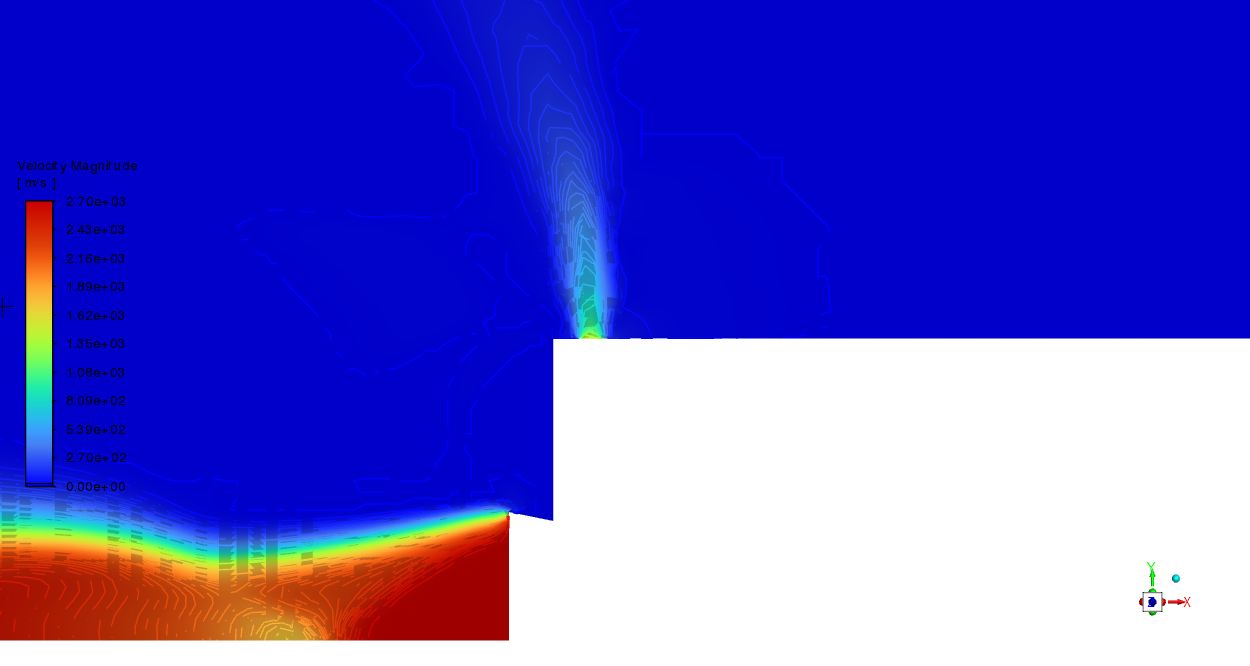
\includegraphics[width=0.495\linewidth]{figs/t0s/vernier_zone_vabs.png}
    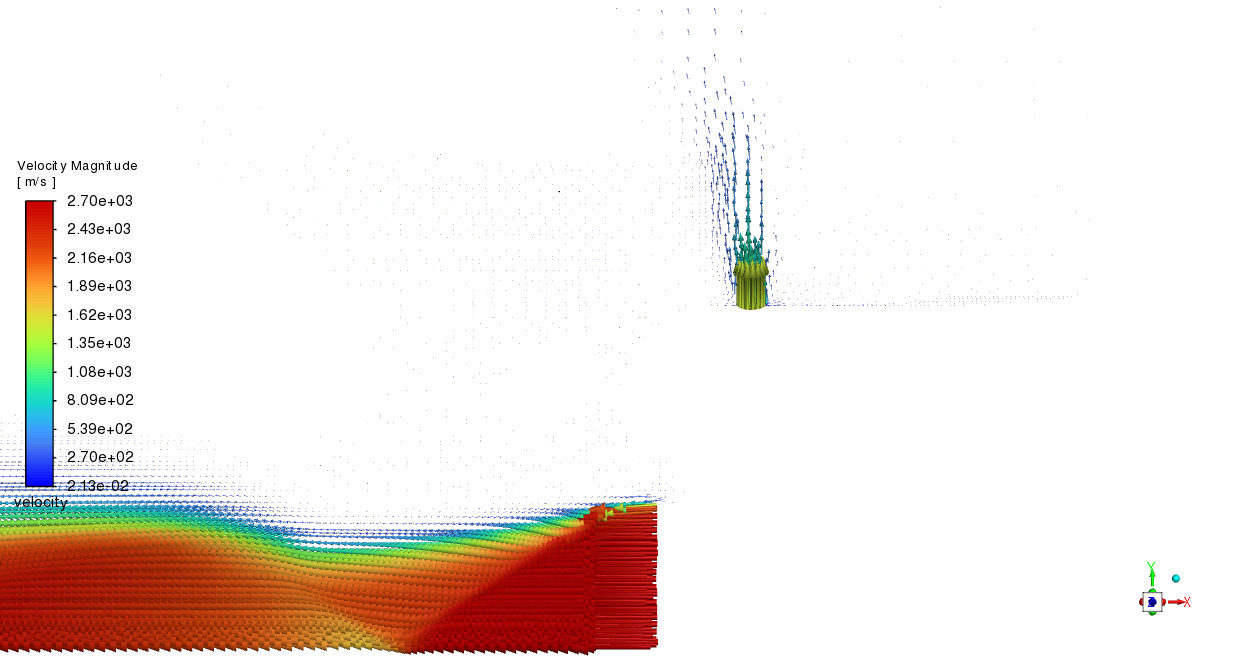
\includegraphics[width=0.495\linewidth]{figs/t0s/vernier_zone_vvabs.png}
    \caption{Velocity magnitude field for the on-on configuration.}
    \label{fig:pabs-conf-modes_t0s}
\end{figure}

\subsubsection*{Pressure field}
%%%%%%%%%%%%%%%%%%%%%%%%%%%%%%%

\begin{figure}[H]
    \centering
    %\includegraphics[width=0.495\linewidth]{figs/t0s/vernier_zone_pabs_offoff.png}
    %\includegraphics[width=0.495\linewidth]{figs/t0s/vernier_zone_pabs_offon.png}\\
    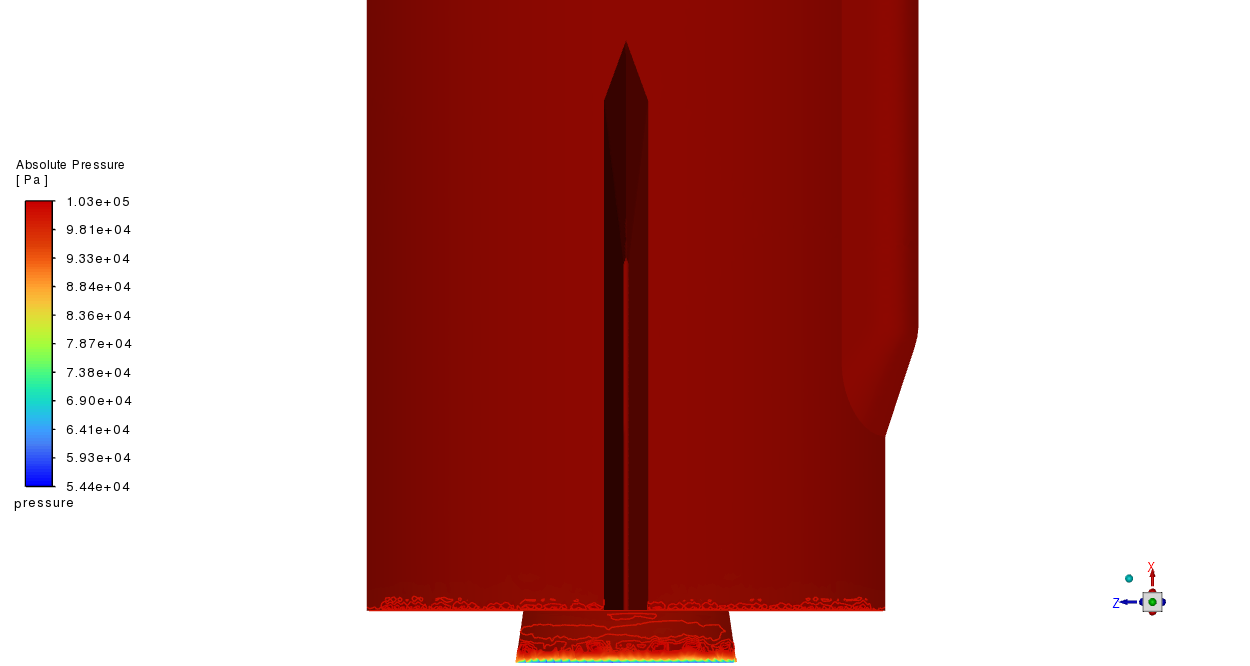
\includegraphics[width=0.495\linewidth]{figs/t0s/vernier_zone_pabs_onoff.png}
    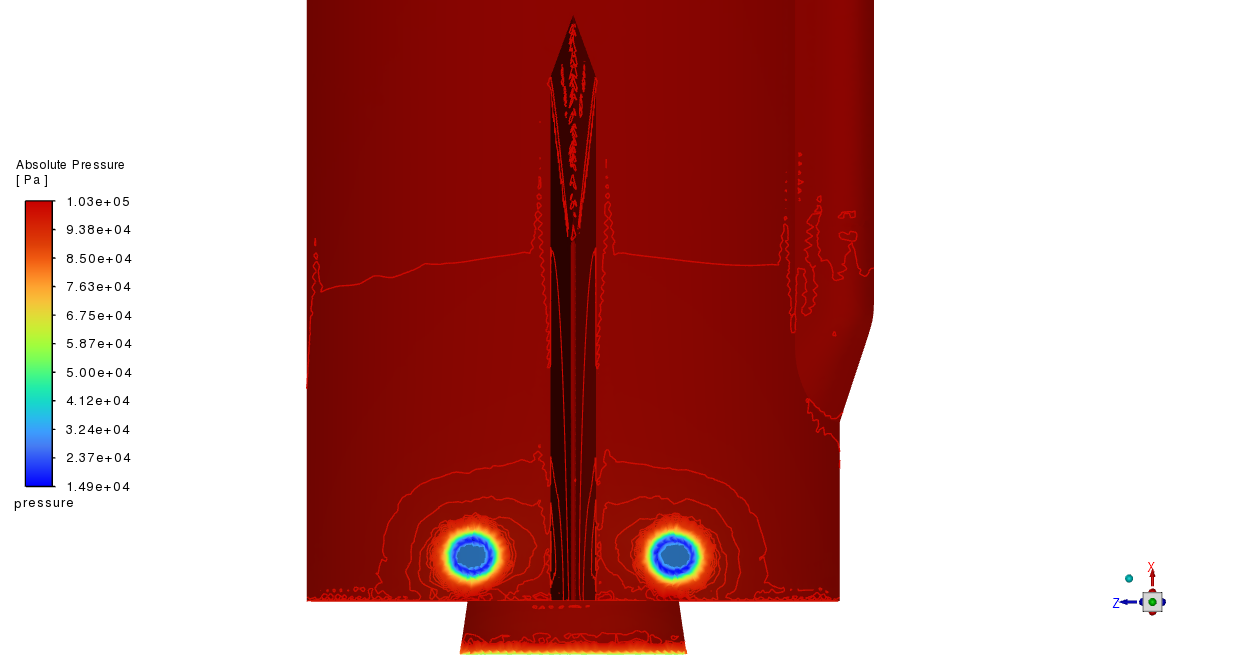
\includegraphics[width=0.495\linewidth]{figs/t0s/vernier_zone_pabs_onon.png}
    \caption{Absolute pressure field: on-off (left) and on-on (right) configuration.}
    \label{fig:pabs-conf-modes_t0s}
\end{figure}

\subsubsection*{Forces and moments}
%%%%%%%%%%%%%%%%%%%%%%%%%%%%%%%%%%%

\begin{table}[H]
\centering
\caption{Moment contributions from different components under various configurations (in Nm) at $t=0s$.}
\resizebox{\textwidth}{!}{%
\begin{tabular}{l r r r r}
\hline
Component        & jetOFF/VernierOFF & jetOFF/VernierON & jetON/VernierOFF & jetON/VernierON \\
\hline
base             &       0.88155149     &      0.077524917     &         115.56513     &          279.23703 \\
fin1             &        1.5041687     &        6.4816512     &         16.010773     &          136.69969 \\
nozzle\_wall     &     -0.014925955     &      -0.38735785     &         -2.6204429    &          -10.048931 \\
pl\_body         &        7.7563575     &        39.210065     &         22.132065     &           79.013722 \\
pl\_fin1         &      -0.45653526     &        2.8477349     &        0.93354685     &           7.1888635 \\
pl\_nose         &       -10.984273     &        8.7627111     &         -2.7111559    &           36.850431 \\
raceway2         &        0.78719102    &        64.066687     &         20.699317     &          156.32869 \\
s01s02s03        &        8.0766737     &        530.10165     &         146.98118     &          1192.9809 \\
s04s05           &       -4.7418678     &        102.57717     &          36.9714      &          255.99597 \\
vernier\_exit1   &     -0.00026325146   &        -             &        0.035683838    &    -                \\
vernier\_exit8   &     -0.00084671014   &        -             &        0.030753828    &    -                \\
\hline
Net Total        &              2.80723 &            753.73784 &           354.02825   &           2134.2464 \\
\hline
\end{tabular}}
\end{table}

%%%%%%%%%%%%%%%%%%%%%%%%%%%%%%%%%%%
\subsection{TC019}\label{sec:TC019}
%%%%%%%%%%%%%%%%%%%%%%%%%%%%%%%%%%%

\subsubsection*{Velocity field}
%%%%%%%%%%%%%%%%%%%%%%%%%%%%%%%

\begin{figure}[H]
    \centering
    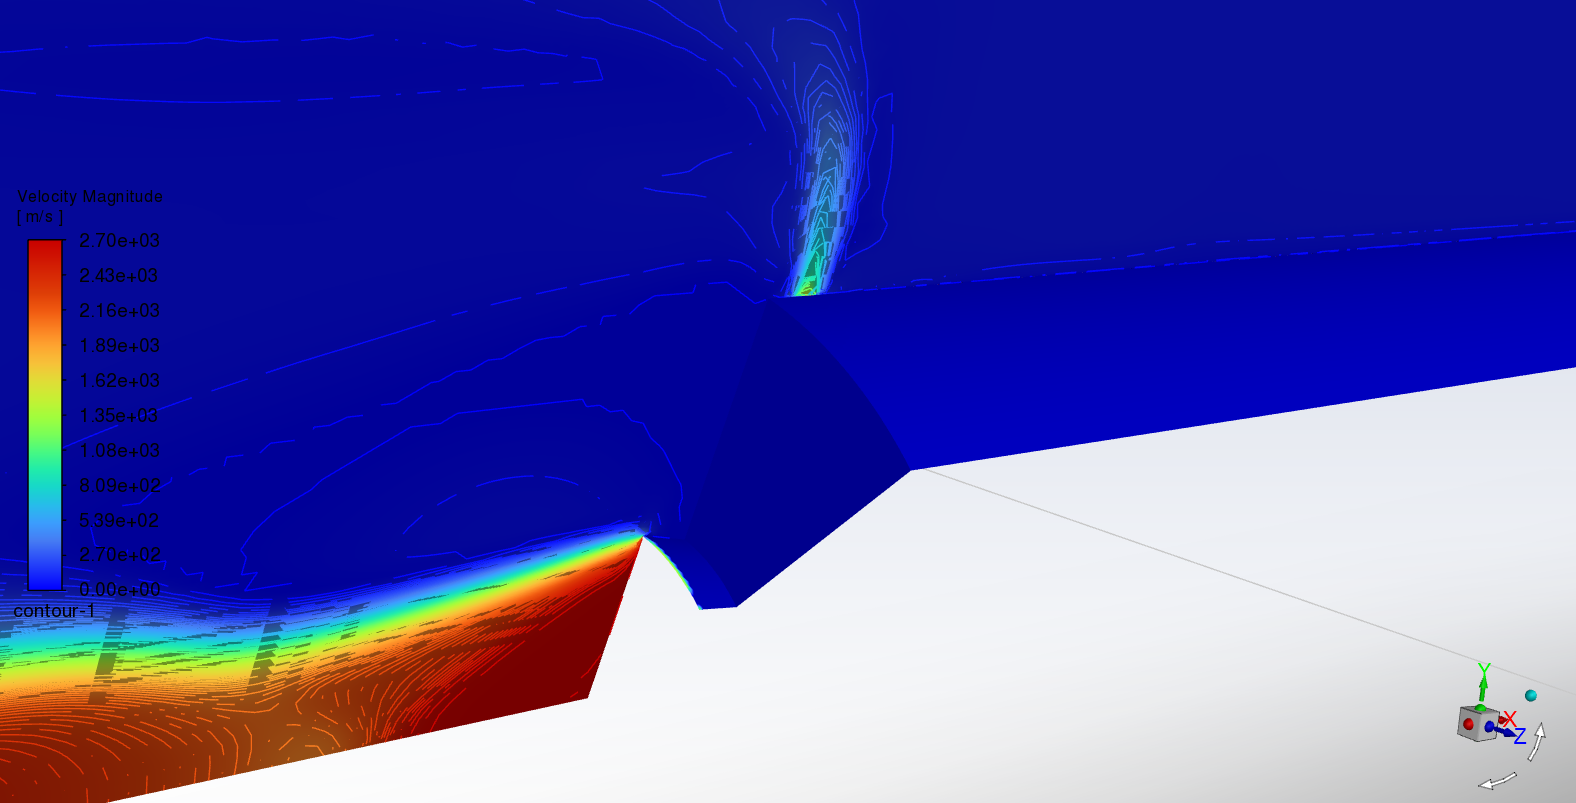
\includegraphics[width=0.495\linewidth]{figs/t19s/magV.png}
    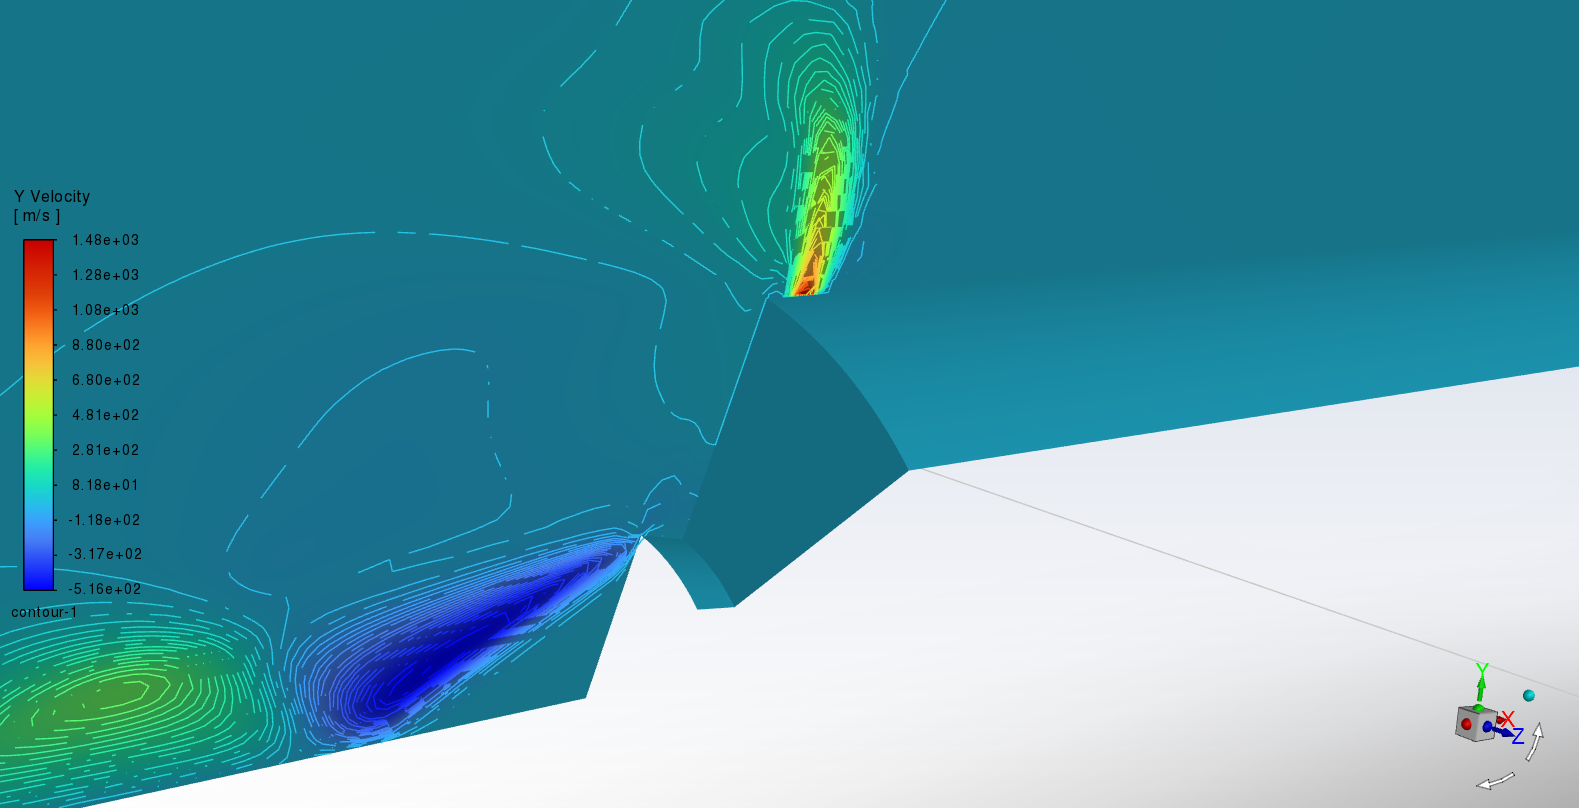
\includegraphics[width=0.495\linewidth]{figs/t19s/v.PNG}
    \caption{Magnitude and transversal velocity field.}
    \label{fig:enter-label}
\end{figure}

\subsubsection*{Pressure field}
%%%%%%%%%%%%%%%%%%%%%%%%%%%%%%%

\begin{figure}[H]
    \centering
    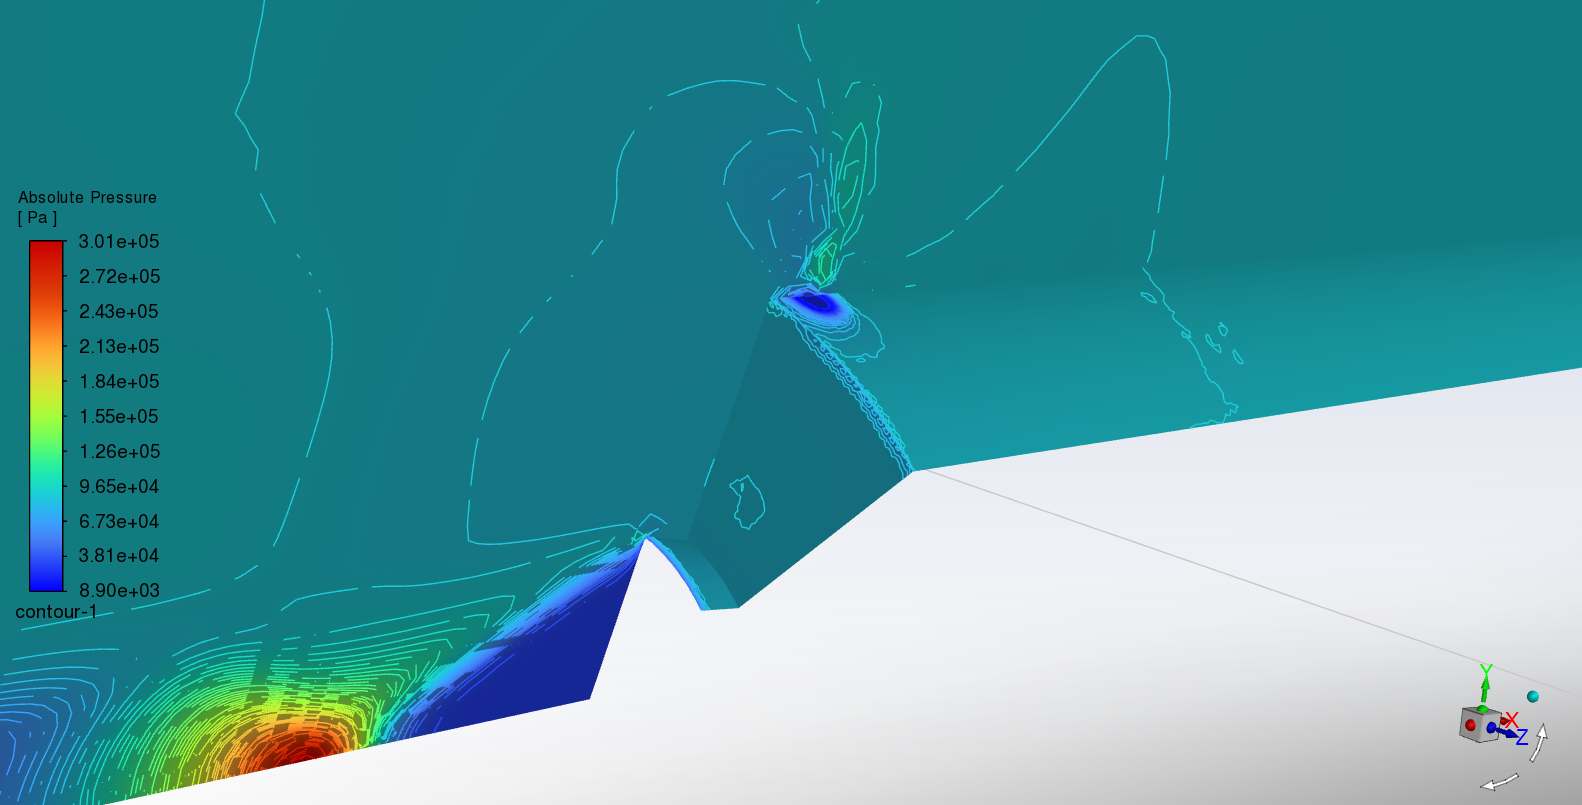
\includegraphics[width=\linewidth]{figs/t19s/pabs.png}
    \caption{Absolute pressure field.}
    \label{fig:enter-label}
\end{figure}

\begin{figure}[H]
    \centering
    \includegraphics[width=0.495\linewidth]{figs/t19s/vernier_zone_pabs_offoff.png}
    \includegraphics[width=0.495\linewidth]{figs/t19s/vernier_zone_pabs_offon.png}\\
    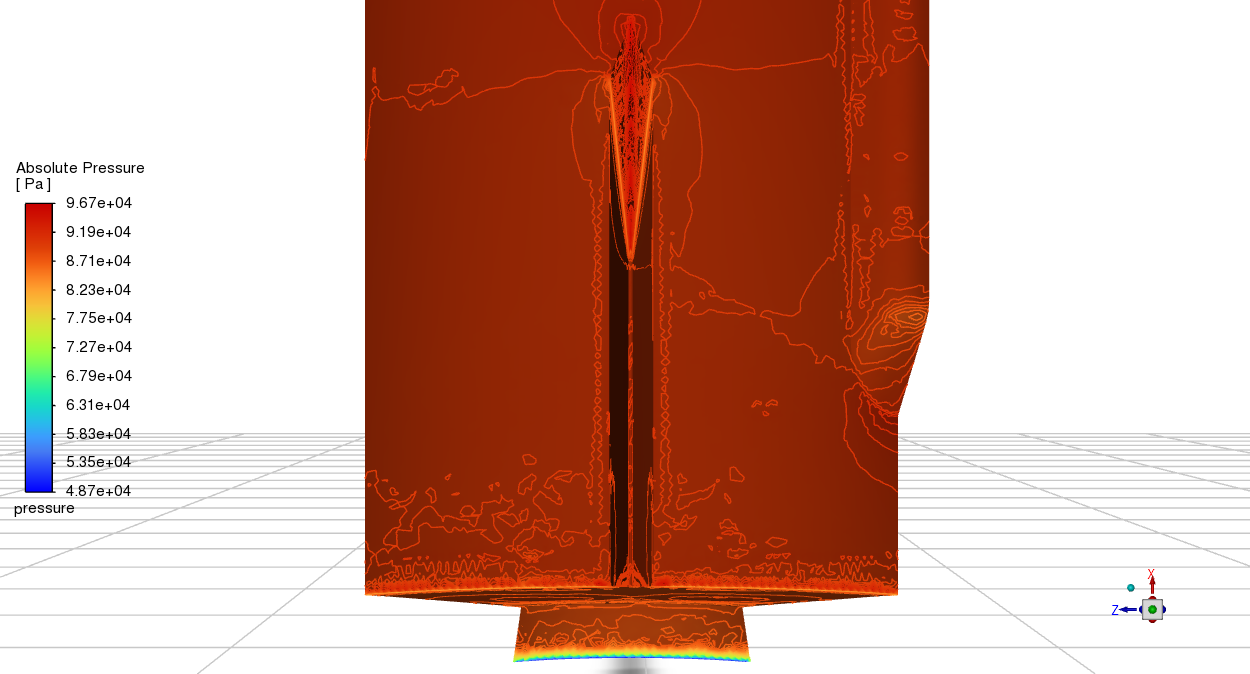
\includegraphics[width=0.495\linewidth]{figs/t19s/vernier_zone_pabs_onoff.png}
    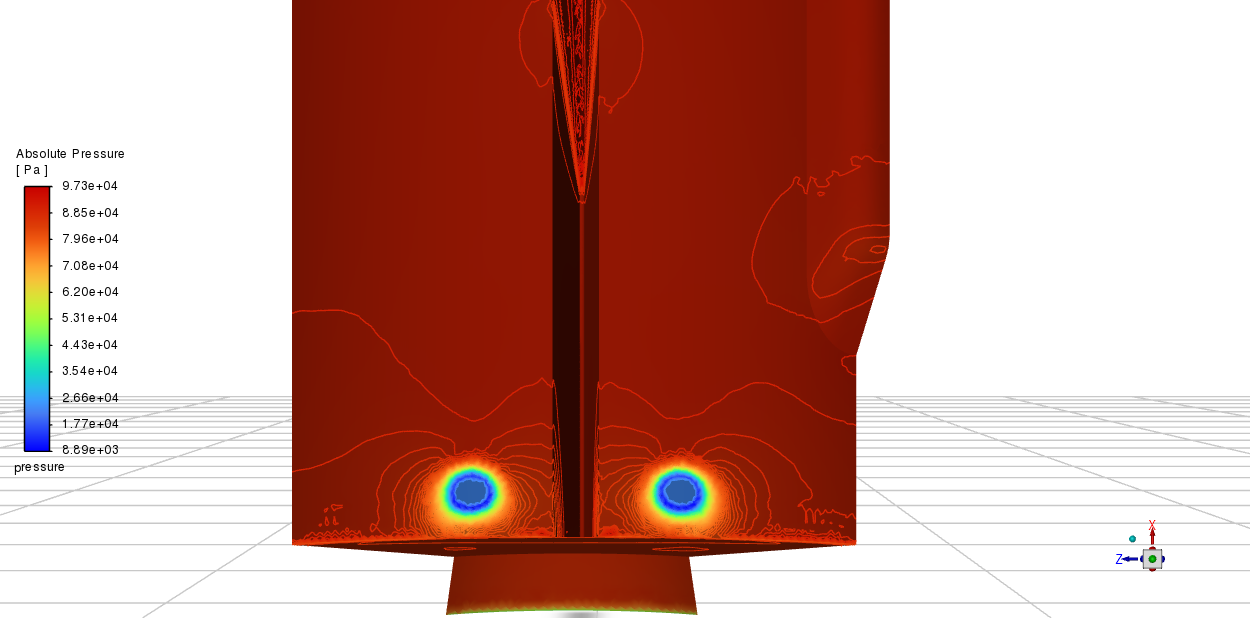
\includegraphics[width=0.495\linewidth]{figs/t19s/vernier_zone_pabs_onon.png}
    \caption{Absolute pressure field. In clockwise order, starting from the upper left corner: off-off, off-on, on-off, on-on configuration.}
    \label{fig:pabs-conf-modes_t19s}
\end{figure}

\subsubsection*{Forces and moments}
%%%%%%%%%%%%%%%%%%%%%%%%%%%%%%%%%%%

\begin{table}[H]
\centering
\caption{Moment contributions from different components under various configurations (in Nm) at $t=19s$ w.r.t. the base.}
\adjustbox{max width=\textwidth}{%
\begin{tabular}{l r r}
\hline
Component           & jetON/VernierOFF & jetON/VernierON \\
\hline
base                & 637.12709        & 833.21848       \\
fin1                & 631.20794        & 719.93726       \\
nozzle\_wall        & -19.732479       & -26.59885       \\
pl\_body            & -1040.7323       & -1084.5408      \\
pl\_fin1            & -250.76179       & -253.7669       \\
pl\_nose            & -933.33831       & -951.48426      \\
raceway2            & 700.08511        & 568.51167       \\
s01s02s03           & 6550.0457        & 5766.6162       \\
s04s05              & -2568.2498       & -2765.9009      \\
vernier\_exit1      & 0.31563891       & —               \\
vernier\_exit8      & 0.26534689       & —               \\
\hline
Net Total           & 3706.2322        & 2805.9919       \\
\hline
\end{tabular}}
\end{table}

%%%%%%%%%%%%%%%%%%%%%%%%%%%%%%%%%%%
\subsection{TC039}\label{sec:TC039}
%%%%%%%%%%%%%%%%%%%%%%%%%%%%%%%%%%%

\subsubsection*{Velocity field}
%%%%%%%%%%%%%%%%%%%%%%%%%%%%%%%

\begin{figure}[H]
    \centering
    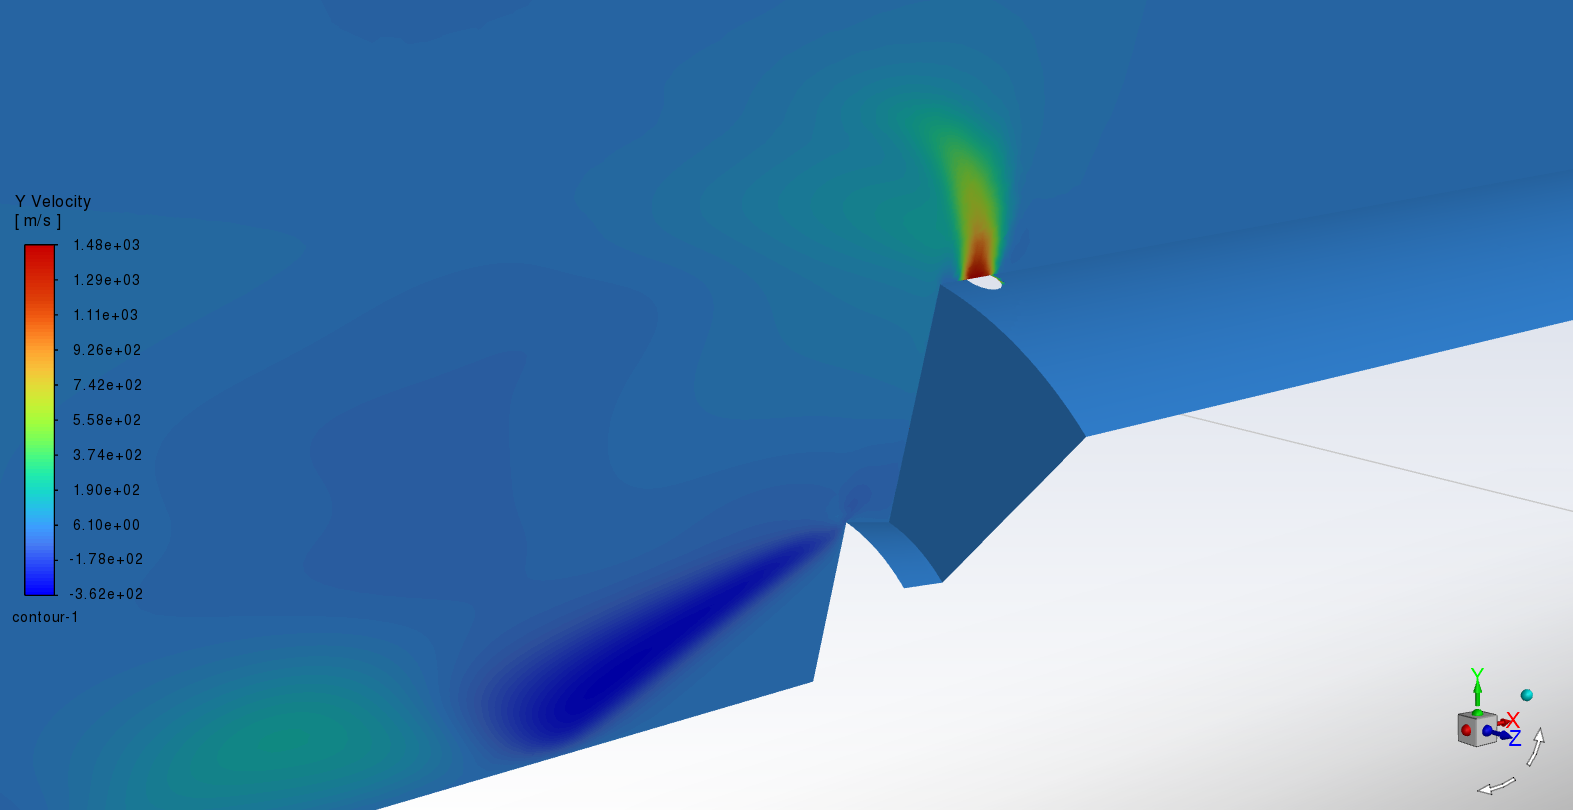
\includegraphics[width=\linewidth]{figs/t39s/V.PNG}
    \caption{Transversal velocity field.}
    \label{fig:enter-label}
\end{figure}

\subsubsection*{Pressure field}
%%%%%%%%%%%%%%%%%%%%%%%%%%%%%%%

\begin{figure}[H]
    \centering
    \includegraphics[width=\linewidth]{figs/t39s/pabs2.PNG}
    \caption{Absolute pressure field.}
    \label{fig:enter-label}
\end{figure}

\begin{figure}[H]
    \centering
    \includegraphics[width=0.495\linewidth]{figs/t39s/vernier_zone_pabs_2_offoff.png}
    \includegraphics[width=0.495\linewidth]{figs/t39s/vernier_zone_pabs_2_offon.png}\\
    \includegraphics[width=0.495\linewidth]{figs/t39s/vernier_zone_pabs_2_onoff.png}
    \includegraphics[width=0.495\linewidth]{figs/t39s/vernier_zone_pabs_2_onon.png}
    \caption{Absolute pressure field. In clockwise order, starting from the upper left corner: off-off, off-on, on-off, on-on configuration.}
    \label{fig:pabs-conf-modes_t39s}
\end{figure}

\subsubsection*{Forces and moments}
%%%%%%%%%%%%%%%%%%%%%%%%%%%%%%%%%%%

\begin{table}[H]
\centering
\caption{Moment contributions from different components under various configurations (in Nm) at $t=39s$ w.r.t. the base.}
\adjustbox{max width=\textwidth}{%
\begin{tabular}{l r r}
\hline
Component           & jetON/VernierOFF & jetON/VernierON \\
\hline
base                & 1332.4979        & 2090.2272       \\
fin1                & 1375.4071        & 1834.8352       \\
nozzle\_wall        & -37.603107       & -62.708175      \\
pl\_body            & -6121.6283       & -4826.0879      \\
pl\_fin1            & -798.22223       & -1017.3771      \\
pl\_nose            & -1749.1138       & -2892.5696      \\
raceway2            & 2489.3424        & 2176.6234       \\
s01s02s03           & 30040.137        & 24872.248       \\
s04s05              & -9138.3195       & -17199.736      \\
vernier\_exit1      & 0.84844054       & —               \\
vernier\_exit8      & 0.76326269       & —               \\
\hline
Net Total           & 17394.109        & 4975.455        \\
\hline
\end{tabular}}
\end{table}

%%%%%%%%%%%%%%%%%%%%%%%%%%%%%%%%%%%
\subsection{TC065}\label{sec:TC065}
%%%%%%%%%%%%%%%%%%%%%%%%%%%%%%%%%%%

\subsubsection*{Velocity field}
%%%%%%%%%%%%%%%%%%%%%%%%%%%%%%

\begin{figure}[H]
    \centering
    \includegraphics[width=0.495\linewidth]{figs/t65s/t65s_V1only_magV2.PNG}
    \includegraphics[width=0.495\linewidth]{figs/t65s/t65s_V1only_v.PNG}
    \caption{Magnitude and transversal velocity field for only one Vernier jet active shooting perpendicularly to the orifice patch.}
    \label{fig:enter-label}
\end{figure}

\begin{figure}[H]
    \centering
    \includegraphics[width=0.495\linewidth]{figs/t65s/t65s_V50_magV.PNG}
    \includegraphics[width=0.495\linewidth]{figs/t65s/t65s_V50_v.PNG}
    \caption{Magnitude and transversal velocity field for the Vernier jet inclined $\pm$50.3$^\circ$ w.r.t. the vertical plane.}
   \label{fig:enter-label}
\end{figure}

\subsubsection*{Pressure field}
%%%%%%%%%%%%%%%%%%%%%%%%%%%%%%

\begin{figure}[H]
    \centering
    \includegraphics[width=0.445\linewidth]{figs/t65s/t65s_V50_pabs.png}
    \includegraphics[width=0.495\linewidth]{figs/t65s/t65s_V1only_pabs.PNG}
    \caption{Absolute pressure field for (left) the Vernier jet inclined $\pm$50.3$^\circ$ w.r.t. the vertical plane and (right) only one Vernier jet active shooting perpendicularly to the orifice patch.}
    \label{fig:enter-label}
\end{figure}

\begin{figure}[H]
    \centering
    \includegraphics[width=0.495\linewidth]{figs/t65s/pressure_contour_plot_xy_plane_with_geometry.png}
    \includegraphics[width=0.495\linewidth]{figs/t65s/pressure_contour_plot_vernier_plane_with_geometry.png}
    \caption{Absolute pressure field on the XY- (left) and Vernier plane (right).}
    \label{fig:enter-label}
\end{figure}

\subsubsection*{Forces and moments}
%%%%%%%%%%%%%%%%%%%%%%%%%%%%%%%%%%%

\begin{table}[H]
\centering
\caption{Moment contributions from different components under various configurations (in Nm) at $t=65s$ w.r.t. the base.}
\adjustbox{max width=\textwidth}{%
\begin{tabular}{l r r r r}
\hline
Component           & jetON/VernierOFF & jetON/VernierON & jetON/VernierON $V_1$ only & jetON/VernierON 50.3$^\circ$ \\
\hline
base                & 1338.6611        & 1857.13         & 1674.3992               & 1787.6806               \\
fin1                & 1449.1521        & 1306.5206       & 1394.0202               & 1349.4822               \\
nozzle\_wall        & -35.620867       & -52.385079      & -46.610018              & -50.536388              \\
pl\_body            & -1896.0933       & -1909.9334      & -1904.1639              & -1909.8347              \\
pl\_fin1            & -635.78906       & -636.31142      & -636.08406              & -636.31808              \\
pl\_nose            & -3795.8175       & -3795.1385      & -3795.419               & -3795.0544              \\
raceway2            & 5402.4696        & 4994.6055       & 5363.9217               & 5048.6162               \\
s01s02s03           & 45617.472        & 42852.367       & 44307.658               & 43258.717               \\
s04s05              & -40503.529       & -40446.276      & -40468.01               & -40446.28               \\
vernier\_exit1      & 0.34398585       & —               & —                       & —                       \\
vernier\_exit8      & 0.26644677       & —               & 0.049599965             & —                       \\
\hline
Net Total           & 6941.5149        & 4170.5784       & 5889.7616               & 4606.4725                \\
\hline
\end{tabular}}
\end{table}

\begin{figure}[H]
    \centering
    \includegraphics[width=0.495\linewidth]{figs/t65s/jetOFFVernierOFF/t65s_M1p08_jetOFFVernierOFF-31-02250_CF.png}
    \includegraphics[width=0.495\linewidth]{figs/t65s/jetOFFVernierON/t65s_M1p08_jetOFFVernieON_Cf.png}\\
    \includegraphics[width=0.495\linewidth]{figs/t65s/jetONVernierOFF/t65s_M1p08_jetONVernierOFF_CF.png}
    \includegraphics[width=0.495\linewidth]{figs/t65s/jetONVernierON/t65s_M1p08_jetONVernierON_CF.png}
    \caption{Pressure coefficient in the Charon's aft region. In clock-wise order from upper left: jetOFF/VernierOFF, jetOFF/VernierON, jetON/VernierOFF, jetON/VernierON.}
    \label{fig:t65s_cp}
\end{figure}

\begin{figure}[H]
    \centering
    \includegraphics[width=0.685\linewidth]{figs/t65s/jetOFFVernierOFF/t65s_M1p08_jetOFFVernierOFF-31-02250_HF.png}\\
    \includegraphics[width=0.685\linewidth]{figs/t65s/jetOFFVernierON/t65s_M1p08_jetOFFVernieON_HF.png}\\
    \includegraphics[width=0.685\linewidth]{figs/t65s/jetONVernierOFF/t65s_M1p08_jetONVernierOFF_HF_full.png}\\
    \includegraphics[width=0.685\linewidth]{figs/t65s/jetONVernierON/t65s_M1p08_jetONVernierON_HF_full.png}
    \caption{Area-average heat flux on Charon's wall surface. From the top: jetOFF/VernierOFF, jetOFF/VernierON, jetON/VernierOFF, jetON/VernierON.}
    \label{fig:t65s_hf}
\end{figure}

%%%%%%%%%%%%%%%%%%%%%%%%%%%%%%%%%%%
\subsection{TC136}\label{sec:TC136}
%%%%%%%%%%%%%%%%%%%%%%%%%%%%%%%%%%%

\subsubsection*{Velocity field}
%%%%%%%%%%%%%%%%%%%%%%%%%%%%%%%

\begin{figure}[H]
    \centering
    \includegraphics[width=0.495\linewidth]{figs/t136s/Vmag.PNG}
    \includegraphics[width=0.495\linewidth]{figs/t136s/V.PNG}
    \caption{Magnitude and transversal velocity field.}
    \label{fig:enter-label}
\end{figure}

\subsubsection*{Pressure field}
%%%%%%%%%%%%%%%%%%%%%%%%%%%%%%%

\begin{figure}[H]
    \centering
    %\includegraphics[width=0.495\linewidth]{figs/t136s/pabs.PNG}
    \includegraphics[width=\linewidth]{figs/t136s/pabs2.PNG}
    \caption{Absolute pressure field.}
    \label{fig:enter-label}
\end{figure}

\begin{figure}[H]
    \centering
    \includegraphics[width=0.495\linewidth]{figs/t136s/vernier_zone_pabs_2_offoff.png}
    \includegraphics[width=0.495\linewidth]{figs/t136s/vernier_zone_pabs_2_offon.png}\\
    \includegraphics[width=0.495\linewidth]{figs/t136s/vernier_zone_pabs_2_onoff.png}
    \includegraphics[width=0.495\linewidth]{figs/t136s/vernier_zone_pabs_2_onon.png}
    \caption{Absolute pressure field. In clockwise order, starting from the upper left corner: off-off, off-on, on-off, on-on configuration.}
    \label{fig:pabs-conf-modes}
\end{figure}

\subsubsection*{Forces and moments}
%%%%%%%%%%%%%%%%%%%%%%%%%%%%%%%%%%%

\begin{table}[H]
\centering
\caption{Moment contributions from different components under various configurations (in Nm) at $t=136s$ w.r.t. the base.}
\adjustbox{max width=\textwidth}{%
\begin{tabular}{l r r}
\hline
Component           & jetON/VernierOFF & jetON/VernierON \\
\hline
base                & 37.773132        & 30.922796       \\
fin1                & 89.445576        & 81.765777       \\
nozzle\_wall        & 0.76689695       & 0.99799816      \\
pl\_body            & 24.994191        & 21.792926       \\
pl\_fin1            & -40.824423       & -41.101857      \\
pl\_nose            & -357.0308        & -361.23343      \\
raceway2            & 2.1781228        & 2.0619345       \\
s01s02s03           & 200.07465        & 174.64171       \\
s04s05              & -4482.0649       & -4482.9294      \\
vernier\_exit1      & 0.054359113      & —               \\
vernier\_exit8      & 0.041661661      & —               \\
\hline
Net Total           & -4524.5916       & -4573.0816      \\
\hline
\end{tabular}}
\end{table}

%%%%%%%%%%%%%%%%%%%%%%%%%%%%%%%%%%%%%%%%%%%%
\section{Conclusions}\label{sec:conclusions}
%%%%%%%%%%%%%%%%%%%%%%%%%%%%%%%%%%%%%%%%%%%%
A campaign of numerical simulation was carried out in order to characterize the role and effects of the Vernier thruster jets on the Charon aft body. In particular, an amplification factor, relevant for controllability purposes, for forces and moments was defined and estimated analyzing the results from several flight trajectory points. The map of the skin pressure was extracted and contour was plotted for the same trajectory points. Based on the values obtained from the numerical simulations, \hl{it was found that the amplification factor for both normal forces and pitch moment never exceeds a value of 2 for the designed flight trajectory attaining a maximum in the hypersonic regime}. %Additional investigation should be devoted to clarify what happens at $t=19~s$ where a higher negative value is obtained.

% Signature
\vspace{\fill}
\begin{center}
    \hspace*{9.0cm} \LARGE \textbf{Lorenzo Campoli} \\
    \hspace*{9.0cm}\includegraphics[width=0.45\textwidth]{signature/signature0.png}
\end{center}

\vspace*{-1.0cm}

\hspace*{9.0cm}\textbf{Senior Systems Modelling Engineer}

\hspace*{9.0cm}\textbf{Gilmour Space Technologies}

\hspace*{9.0cm}\textbf{lorenzo.campoli@gspace.com}

\newpage
\nocite{*}
\bibliography{refs/refs}
\bibliographystyle{unsrt}

\end{document}